\section{Supplementary material}

\subsection{Descriptive statistics}

\small
\renewcommand{\arraystretch}{1.3}
\begin{longtable}{p{7cm} p{1cm} p{0.8cm} p{0.8cm} p{0.8cm} p{0.8cm} p{0.8cm} p{0.8cm} p{0.8cm} p{0.8cm}}
\caption{Descriptive statistics for all patients arriving at each stroke team. The table shows summary statistics across all stroke teams.}\\
\toprule
\endhead
Statistic & Stroke teams & mean & Std Dev & min & 25\% & 50\% & 75\% & max\tabularnewline
\midrule
Yearly admissions & 119 & 509 & 208 & 95 & 372 & 489 & 627 & 1183\tabularnewline
Age (mean) & 119 & 74 & 2 & 65 & 73 & 75 & 76 & 78\tabularnewline
Proportion aged 80+ & 119 & 0.40 & 0.06 & 0.20 & 0.36 & 0.40 & 0.44 & 0.51\tabularnewline
Proportion male & 119 & 0.53 & 0.02 & 0.47 & 0.51 & 0.53 & 0.55 & 0.60\tabularnewline
Prior disability (mRS, mean) & 119 & 1.02 & 0.25 & 0.29 & 0.87 & 1.03 & 1.21 & 1.60\tabularnewline
Proportion prior disability (mRS) 0-2 & 119 & 0.81 & 0.05 & 0.67 & 0.78 & 0.81 & 0.84 & 0.97\tabularnewline
Proportion ischaemic stroke & 119 & 0.88 & 0.02 & 0.83 & 0.86 & 0.88 & 0.89 & 0.93\tabularnewline
Stroke severity (NIHSS, mean) & 119 & 7.0 & 1.0 & 4.6 & 6.3 & 7.2 & 7.8 & 9.1\tabularnewline
Proportion with known onset & 119 & 0.68 & 0.14 & 0.43 & 0.58 & 0.67 & 0.76 & 1.00\tabularnewline
Onset-to-arrival time (minutes, median) & 119 & 204 & 76 & 109 & 155 & 180 & 224 & 466\tabularnewline
Proportion arriving within 4 hours known onset & 119 & 0.38 & 0.06 & 0.19 & 0.34 & 0.38 & 0.43 & 0.51\tabularnewline
Proportion with precisely known onset & 119 & 0.33 & 0.11 & 0.01 & 0.28 & 0.34 & 0.39 & 0.63\tabularnewline
Proportion onset during sleep & 119 & 0.14 & 0.06 & 0.00 & 0.09 & 0.14 & 0.17 & 0.34\tabularnewline
Proportion arrive by ambulance & 119 & 0.78 & 0.07 & 0.47 & 0.76 & 0.79 & 0.82 & 0.92\tabularnewline
Call-to-ambulance arrival time (minutes, median) & 113 & 22 & 10 & 13 & 17 & 20 & 24 & 103\tabularnewline
Ambulance on scene time (median) & 113 & 31 & 3 & 20 & 28 & 31 & 33 & 41\tabularnewline
Ambulance conveyance time (minutes, median) & 113 & 18 & 5 & 10 & 15 & 17 & 21 & 37\tabularnewline
Arrival-to-scan time (minutes, median) & 119 & 53 & 21 & 13 & 39 & 51 & 63 & 129\tabularnewline
Proportion receiving thrombolysis & 119 & 0.115 & 0.034 & 0.021 & 0.092 & 0.110 & 0.136 & 0.245\tabularnewline
Scan-to-thrombolysis time (minutes, median) & 119 & 34 & 10 & 14 & 28 & 34 & 41 & 72\tabularnewline
Discharge disability (mRS, mean) & 119 & 2.641 & 0.352 & 1.361 & 2.413 & 2.699 & 2.900 & 3.320\tabularnewline
Proportion discharged mRS 0-2 & 119 & 0.524 & 0.095 & 0.293 & 0.454 & 0.522 & 0.594 & 0.799\tabularnewline
Proportion discharged mRS 5-6 & 119 & 0.195 & 0.037 & 0.095 & 0.170 & 0.198 & 0.218 & 0.287\tabularnewline
\bottomrule
\label{tab:hospital_stats_1}
\end{longtable}
\normalsize

\small
\begin{longtable}{p{7cm} p{1cm} p{0.8cm} p{0.8cm} p{0.8cm} p{0.8cm} p{0.8cm} p{0.8cm} p{0.8cm} p{0.8cm}}
\caption{Descriptive statistics for patients arriving at each stroke team, for patients arriving within 4 hours of known stroke onset. The table shows summary statistics across all stroke teams.}\\
\toprule
\endhead
Statistic & Stroke teams & mean & Std Dev & min & 25\% & 50\% & 75\% & max\tabularnewline
\midrule
Yearly admissions & 119 & 193 & 78 & 28 & 139 & 183 & 241 & 428\tabularnewline
Age (mean) & 119 & 75 & 2 & 66 & 73 & 75 & 76 & 79\tabularnewline
Proportion aged 80+ & 119 & 0.41 & 0.06 & 0.23 & 0.37 & 0.41 & 0.45 & 0.57\tabularnewline
Proportion male & 119 & 0.53 & 0.03 & 0.45 & 0.51 & 0.53 & 0.55 & 0.64\tabularnewline
Prior disability (mRS, mean) & 119 & 1.04 & 0.25 & 0.37 & 0.88 & 1.04 & 1.22 & 1.60\tabularnewline
Proportion prior disability (mRS) 0-2 & 119 & 0.80 & 0.06 & 0.66 & 0.77 & 0.81 & 0.83 & 0.95\tabularnewline
Proportion ischaemic stroke & 119 & 0.85 & 0.03 & 0.75 & 0.84 & 0.85 & 0.87 & 0.94\tabularnewline
Stroke severity (NIHSS, mean) & 119 & 8.9 & 1.1 & 6.4 & 8.2 & 9.0 & 9.7 & 11.4\tabularnewline
Proportion with known onset & 119 & 1.00 & 0.00 & 1.00 & 1.00 & 1.00 & 1.00 & 1.00\tabularnewline
Onset-to-arrival time (minutes, median) & 119 & 105 & 9 & 85 & 100 & 105 & 111 & 132\tabularnewline
Proportion arriving within 4 hours known onset & 119 & 1.00 & 0.00 & 1.00 & 1.00 & 1.00 & 1.00 & 1.00\tabularnewline
Proportion with precisely known onset & 119 & 0.62 & 0.17 & 0.02 & 0.54 & 0.66 & 0.75 & 0.91\tabularnewline
Proportion onset during sleep & 119 & 0.05 & 0.05 & 0.00 & 0.01 & 0.03 & 0.06 & 0.30\tabularnewline
Proportion arrive by ambulance & 119 & 0.89 & 0.07 & 0.54 & 0.87 & 0.91 & 0.93 & 0.98\tabularnewline
Call-to-ambulance arrival time (minutes, median) & 110 & 19 & 5 & 8 & 16 & 18 & 21 & 51\tabularnewline
Ambulance on scene time (median) & 110 & 28 & 4 & 20 & 26 & 28 & 31 & 46\tabularnewline
Ambulance conveyance time (minutes, median) & 110 & 17 & 4 & 9 & 14 & 16 & 20 & 28\tabularnewline
Arrival-to-scan time (minutes, median) & 119 & 27 & 11 & 4 & 21 & 28 & 34 & 100\tabularnewline
Proportion receiving thrombolysis & 119 & 0.293 & 0.070 & 0.111 & 0.250 & 0.282 & 0.333 & 0.534\tabularnewline
Scan-to-thrombolysis time (minutes, median) & 119 & 34 & 10 & 14 & 28 & 34 & 40 & 71\tabularnewline
Discharge disability (mRS, mean) & 119 & 2.803 & 0.353 & 1.507 & 2.609 & 2.837 & 3.039 & 3.663\tabularnewline
Proportion discharged mRS 0-2 & 119 & 0.494 & 0.094 & 0.209 & 0.424 & 0.495 & 0.554 & 0.771\tabularnewline
Proportion discharged mRS 5-6 & 119 & 0.236 & 0.045 & 0.138 & 0.208 & 0.231 & 0.256 & 0.420\tabularnewline
\bottomrule
\label{tab:hospital_stats_2}
\end{longtable}
\normalsize

\small
\begin{longtable}{p{7cm} p{1cm} p{0.8cm} p{0.8cm} p{0.8cm} p{0.8cm} p{0.8cm} p{0.8cm} p{0.8cm} p{0.8cm}}
\caption{Descriptive statistics for patients arriving at each stroke team, for patients arriving by ambulance within 4 hours of known stroke onset. The table shows summary statistics across all stroke teams.}\\
\toprule
\endhead
Statistic & Stroke teams & mean & Std Dev & min & 25\% & 50\% & 75\% & max\tabularnewline
\midrule
Yearly admissions & 119 & 173 & 74 & 15 & 125 & 163 & 227 & 400\tabularnewline
Age (mean) & 119 & 75 & 2 & 66 & 74 & 76 & 77 & 81\tabularnewline
Proportion aged 80+ & 119 & 0.43 & 0.06 & 0.24 & 0.39 & 0.43 & 0.47 & 0.62\tabularnewline
Proportion male & 119 & 0.52 & 0.03 & 0.45 & 0.51 & 0.52 & 0.54 & 0.60\tabularnewline
Prior disability (mRS, mean) & 119 & 1.10 & 0.25 & 0.46 & 0.94 & 1.09 & 1.26 & 1.66\tabularnewline
Proportion prior disability (mRS) 0-2 & 119 & 0.79 & 0.06 & 0.65 & 0.75 & 0.79 & 0.83 & 0.93\tabularnewline
Proportion ischaemic stroke & 119 & 0.85 & 0.03 & 0.75 & 0.83 & 0.85 & 0.87 & 0.94\tabularnewline
Stroke severity (NIHSS, mean) & 119 & 9.4 & 1.2 & 6.7 & 8.6 & 9.5 & 10.2 & 12.2\tabularnewline
Proportion with known onset & 119 & 1.00 & 0.00 & 1.00 & 1.00 & 1.00 & 1.00 & 1.00\tabularnewline
Onset-to-arrival time (minutes, median) & 119 & 106 & 10 & 84 & 99 & 105 & 112 & 151\tabularnewline
Proportion arriving within 4 hours known onset & 119 & 1.00 & 0.00 & 1.00 & 1.00 & 1.00 & 1.00 & 1.00\tabularnewline
Proportion with precisely known onset & 119 & 0.62 & 0.17 & 0.02 & 0.54 & 0.65 & 0.75 & 0.92\tabularnewline
Proportion onset during sleep & 119 & 0.05 & 0.05 & 0.00 & 0.01 & 0.03 & 0.06 & 0.33\tabularnewline
Proportion arrive by ambulance & 119 & 1.00 & 0.00 & 1.00 & 1.00 & 1.00 & 1.00 & 1.00\tabularnewline
Call-to-ambulance arrival time (minutes, median) & 110 & 19 & 5 & 8 & 16 & 18 & 21 & 51\tabularnewline
Ambulance on scene time (median) & 110 & 28 & 4 & 20 & 26 & 28 & 31 & 46\tabularnewline
Ambulance conveyance time (minutes, median) & 110 & 17 & 4 & 9 & 14 & 16 & 20 & 28\tabularnewline
Arrival-to-scan time (minutes, median) & 119 & 26 & 11 & 4 & 20 & 25 & 33 & 95\tabularnewline
Proportion receiving thrombolysis & 119 & 0.300 & 0.072 & 0.130 & 0.252 & 0.289 & 0.345 & 0.537\tabularnewline
Scan-to-thrombolysis time (minutes, median) & 119 & 34 & 10 & 13 & 27 & 33 & 40 & 73\tabularnewline
Discharge disability (mRS, mean) & 119 & 2.926 & 0.352 & 1.867 & 2.717 & 2.928 & 3.150 & 3.819\tabularnewline
Proportion discharged mRS 0-2 & 119 & 0.465 & 0.096 & 0.184 & 0.398 & 0.462 & 0.524 & 0.696\tabularnewline
Proportion discharged mRS 5-6 & 119 & 0.254 & 0.051 & 0.147 & 0.221 & 0.253 & 0.280 & 0.486\tabularnewline
\bottomrule
\label{tab:hospital_stats_3}
\end{longtable}
\normalsize


\subsection{Feature selection}

\textbf{Summary of findings}

Model with all features
The model performance with all 58 features is:
* AUC: 0.818 (std across 5 kfolds: 0.001)
* Accuracy: 0.440 (std across 5 kfolds: 0.002)
* Accuracy within one: 0.760 (std across 5 kfolds: 0.002)

\textbf{Sequentially selecting features}
Sequentially chose features up to 25 features. We saw that once 14 features we selected, the model choose a feature (infarction) that is the same value for all patients, hence no more information was being obtained beyond this point:
Feature  1: prior\_disability, AUC: 0.687
Feature  2: stroke\_severity, AUC: 0.770
Feature  3: stroke\_team, AUC: 0.800
Feature  4: age, AUC: 0.806
Feature  5: year, AUC: 0.811
Feature  6: nihss\_arrival\_loc, AUC: 0.814
Feature  7: scan\_to\_thrombolysis\_time, AUC: 0.816
Feature  8: thrombolysis\_no\_but\_improving, AUC: 0.817
Feature  9: nihss\_arrival\_best\_language, AUC: 0.818
Feature 10: new\_afib\_diagnosis, AUC: 0.818
Feature 11: nihss\_arrival\_sensory, AUC: 0.819
Feature 12: atrial\_fibrillation, AUC: 0.819
Feature 13: nihss\_arrival\_facial\_palsy, AUC: 0.819
Feature 14: thrombolysis\_no\_but\_other\_medical, AUC: 0.819
Feature 15: infarction, AUC: 0.819
Feature 16: arrive\_by\_ambulance, AUC: 0.819
Feature 17: nihss\_arrival\_motor\_arm\_left, AUC: 0.819
Feature 18: thrombolysis\_no\_but\_comorbidity, AUC: 0.819
Feature 19: nihss\_arrival\_loc\_questions, AUC: 0.819
Feature 20: nihss\_arrival\_motor\_arm\_right, AUC: 0.819
Feature 21: nihss\_arrival\_best\_gaze, AUC: 0.820
Feature 22: thrombolysis\_no\_but\_too\_mild\_severe, AUC: 0.820
Feature 23: diabetes, AUC: 0.820
Feature 24: thrombolysis\_no\_but\_haemorrhagic, AUC: 0.820
Feature 25: thrombolysis\_no\_but\_medication, AUC: 0.820

\textbf{Features chosen for the predictive model}
We will include these 7 features in our model (reasoning given below):
Feature  1: prior\_disability
Feature  2: stroke\_severity
Feature  3: stroke\_team
Feature  4: age
Feature  5: onset\_to\_thrombolysis\_time
Feature  6: any\_afib\_diagnosis
Feature  7: precise\_onset\_known

\textbf{Additional experiments to inform choice of features}

To inform us further about which features to include in our model, we carried out some additional experiments (in other notebooks). Here is what we learnt, and our feature selection choice based on this.

\textbf{Why we chose these 7 features:}
* prior\_disability (easy selection choice)
* stroke\_severity (checked the impact of using the separate NIHSS features instead - decided including stroke severity captured the information)
* stroke\_team (easy selection choice)
* age (easy selection choice)
* onset\_to\_thrombolysis\_time (scan\_to\_thrombolysis\_time is a selected feature, however the feature onset-to-thrombolysis time is a more useful feature to include as it aligns with other research and the clinical focus.We compared the SHAP plots from models that included either (and neither) of these duration features. Across the three models, the other features (age, prior disability, stroke severity) are not affected by the inclusion of either duration feature, nor is any performance accuracy lost)
* any\_afib\_diagnosis (Both new\_afib\_diagnosis and atrial\_fibrillation featrures are in the list above, and we have seen that an atrial fibrillation diagnosis contributes for the mRS6 outcome. We will include any\_afib\_diagnosis as this includes both of the other atrial fibrillation features information. We compared the SHAP plots from models that included one of these atrial fibrillation diagnosis features (and none). Across those models, the other features (age, prior disability, stroke severity) are not affected by the inclusion of which atrial fibrillation feature, nor is any performance accuracy lost).
* precise\_onset\_known (Not included in the feature selection list, however may be useful to include so people can see whether it makes a significant difference to outcomes, as this is often a discussion point amongst clinicians)

\textbf{Why we didn't include these features:}
* YEAR: Any data from beyond 2021 (the latest year in the dataset), the model has yet to see any information about that year. If the decision tree treats the ”Year” feature as a numerical value, any future year will be grouped along with year 2021 for each split - check how the model is treating the Year feature.

We reran feature selection excluding the feature "stroke team" as an option. The feature "Year" was now not a selected features. Here are those results:

There are 56 features
All features, AUC: 0.786 (std across 5 kfolds: 0.001)
All features, accuracy: 0.387 (std across 5 kfolds: 0.003)
All features, accuracy within one: 0.734 (std across 5 kfolds: 0.003)

Feature  1: prior\_disability, AUC: 0.687
Feature  2: stroke\_severity, AUC: 0.770
Feature  3: age, AUC: 0.777
Feature  4: nihss\_arrival\_loc, AUC: 0.779
Feature  5: scan\_to\_thrombolysis\_time, AUC: 0.780
Feature  6: thrombolysis\_no\_but\_improving, AUC: 0.782
Feature  7: nihss\_arrival\_best\_language, AUC: 0.783
Feature  8: thrombolysis\_no\_but\_other\_medical, AUC: 0.783
Feature  9: nihss\_arrival\_sensory, AUC: 0.784
Feature 10: nihss\_arrival\_facial\_palsy, AUC: 0.784
Feature 11: nihss\_arrival\_limb\_ataxia, AUC: 0.784
Feature 12: nihss\_arrival\_motor\_arm\_left, AUC: 0.785
Feature 13: nihss\_arrival\_best\_gaze, AUC: 0.785
Feature 14: diabetes, AUC: 0.785
Feature 15: thrombolysis\_no\_but\_comorbidity, AUC: 0.785
Feature 16: nihss\_arrival\_motor\_arm\_right, AUC: 0.786
Feature 17: thrombolysis\_no\_but\_too\_mild\_severe, AUC: 0.786
Feature 18: onset\_during\_sleep, AUC: 0.786
Feature 19: precise\_onset\_known, AUC: 0.786
Feature 20: atrial\_fibrillation, AUC: 0.786
Feature 21: infarction, AUC: 0.786
Feature 22: arrive\_by\_ambulance, AUC: 0.786
Feature 23: nihss\_complete, AUC: 0.786
Feature 24: prior\_stroke\_tia, AUC: 0.786
Feature 25: nihss\_arrival\_dysarthria, AUC: 0.786

To investigate the interaction between "stroke team" and "year" we created some binary models (as SHAP interaction can not be calculated for a multiclass model). This showed that ....

* Individual NIHSS features are not included, as we are already including the feature stroke severity, and this is dependent on the individual NIHSS features (SHAP required features to be independant, apart from with the target feature)
* scan\_to\_thrombolysis\_time is being represented by the feature onset\_to\_thrombolysis\_time
* atrial\_fibrillation and new\_afib\_dianosis are being represented by the feature any\_afib\_diagnosis
* thrombolysis\_no\_but\_improving (there is a messiness of this feature overlapping with the onset\_to\_thrombolysis\_time. We would now have two features saying that the patient does not receive IVT).
* thrombolysis\_no\_but\_other\_medical (the SHAP plots show that this feature does not have a big effect on predicting the outcome).

Figure \ref{fig:feature_selection} shows the mean ROCAUC for the 5 kfold model, sequentially selecting the features.
\begin{figure}[!h]
    \centering
    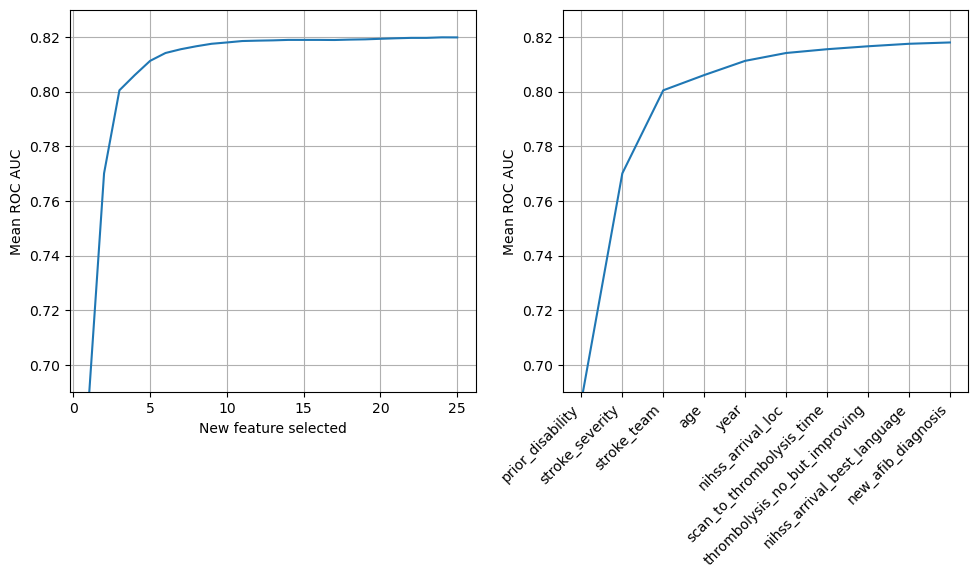
\includegraphics[width=0.75\textwidth]{./images/020_feature_selection.jpg}\\
    \caption{Feature selection}
    \label{fig:feature_selection}
\end{figure}


\subsection{Feature selection}

\textbf{Summary of findings}

Model with all features
The model performance with all 58 features is:
* AUC: 0.818 (std across 5 kfolds: 0.001)
* Accuracy: 0.440 (std across 5 kfolds: 0.002)
* Accuracy within one: 0.760 (std across 5 kfolds: 0.002)

\textbf{Sequentially selecting features}
Sequentially chose features up to 25 features. We saw that once 14 features we selected, the model choose a feature (infarction) that is the same value for all patients, hence no more information was being obtained beyond this point:
Feature  1: prior\_disability, AUC: 0.687
Feature  2: stroke\_severity, AUC: 0.770
Feature  3: stroke\_team, AUC: 0.800
Feature  4: age, AUC: 0.806
Feature  5: year, AUC: 0.811
Feature  6: nihss\_arrival\_loc, AUC: 0.814
Feature  7: scan\_to\_thrombolysis\_time, AUC: 0.816
Feature  8: thrombolysis\_no\_but\_improving, AUC: 0.817
Feature  9: nihss\_arrival\_best\_language, AUC: 0.818
Feature 10: new\_afib\_diagnosis, AUC: 0.818
Feature 11: nihss\_arrival\_sensory, AUC: 0.819
Feature 12: atrial\_fibrillation, AUC: 0.819
Feature 13: nihss\_arrival\_facial\_palsy, AUC: 0.819
Feature 14: thrombolysis\_no\_but\_other\_medical, AUC: 0.819
Feature 15: infarction, AUC: 0.819
Feature 16: arrive\_by\_ambulance, AUC: 0.819
Feature 17: nihss\_arrival\_motor\_arm\_left, AUC: 0.819
Feature 18: thrombolysis\_no\_but\_comorbidity, AUC: 0.819
Feature 19: nihss\_arrival\_loc\_questions, AUC: 0.819
Feature 20: nihss\_arrival\_motor\_arm\_right, AUC: 0.819
Feature 21: nihss\_arrival\_best\_gaze, AUC: 0.820
Feature 22: thrombolysis\_no\_but\_too\_mild\_severe, AUC: 0.820
Feature 23: diabetes, AUC: 0.820
Feature 24: thrombolysis\_no\_but\_haemorrhagic, AUC: 0.820
Feature 25: thrombolysis\_no\_but\_medication, AUC: 0.820

\textbf{Features chosen for the predictive model}
We will include these 7 features in our model (reasoning given below):
Feature  1: prior\_disability
Feature  2: stroke\_severity
Feature  3: stroke\_team
Feature  4: age
Feature  5: onset\_to\_thrombolysis\_time
Feature  6: any\_afib\_diagnosis
Feature  7: precise\_onset\_known

\textbf{Additional experiments to inform choice of features}

To inform us further about which features to include in our model, we carried out some additional experiments (in other notebooks). Here is what we learnt, and our feature selection choice based on this.

\textbf{Why we chose these 7 features:}
* prior\_disability (easy selection choice)
* stroke\_severity (checked the impact of using the separate NIHSS features instead - decided including stroke severity captured the information)
* stroke\_team (easy selection choice)
* age (easy selection choice)
* onset\_to\_thrombolysis\_time (scan\_to\_thrombolysis\_time is a selected feature, however the feature onset-to-thrombolysis time is a more useful feature to include as it aligns with other research and the clinical focus.We compared the SHAP plots from models that included either (and neither) of these duration features. Across the three models, the other features (age, prior disability, stroke severity) are not affected by the inclusion of either duration feature, nor is any performance accuracy lost)
* any\_afib\_diagnosis (Both new\_afib\_diagnosis and atrial\_fibrillation featrures are in the list above, and we have seen that an atrial fibrillation diagnosis contributes for the mRS6 outcome. We will include any\_afib\_diagnosis as this includes both of the other atrial fibrillation features information. We compared the SHAP plots from models that included one of these atrial fibrillation diagnosis features (and none). Across those models, the other features (age, prior disability, stroke severity) are not affected by the inclusion of which atrial fibrillation feature, nor is any performance accuracy lost).
* precise\_onset\_known (Not included in the feature selection list, however may be useful to include so people can see whether it makes a significant difference to outcomes, as this is often a discussion point amongst clinicians)

\textbf{Why we didn't include these features:}
* YEAR: Any data from beyond 2021 (the latest year in the dataset), the model has yet to see any information about that year. If the decision tree treats the ”Year” feature as a numerical value, any future year will be grouped along with year 2021 for each split - check how the model is treating the Year feature.

We reran feature selection excluding the feature "stroke team" as an option. The feature "Year" was now not a selected features. Here are those results:

There are 56 features
All features, AUC: 0.786 (std across 5 kfolds: 0.001)
All features, accuracy: 0.387 (std across 5 kfolds: 0.003)
All features, accuracy within one: 0.734 (std across 5 kfolds: 0.003)

Feature  1: prior\_disability, AUC: 0.687
Feature  2: stroke\_severity, AUC: 0.770
Feature  3: age, AUC: 0.777
Feature  4: nihss\_arrival\_loc, AUC: 0.779
Feature  5: scan\_to\_thrombolysis\_time, AUC: 0.780
Feature  6: thrombolysis\_no\_but\_improving, AUC: 0.782
Feature  7: nihss\_arrival\_best\_language, AUC: 0.783
Feature  8: thrombolysis\_no\_but\_other\_medical, AUC: 0.783
Feature  9: nihss\_arrival\_sensory, AUC: 0.784
Feature 10: nihss\_arrival\_facial\_palsy, AUC: 0.784
Feature 11: nihss\_arrival\_limb\_ataxia, AUC: 0.784
Feature 12: nihss\_arrival\_motor\_arm\_left, AUC: 0.785
Feature 13: nihss\_arrival\_best\_gaze, AUC: 0.785
Feature 14: diabetes, AUC: 0.785
Feature 15: thrombolysis\_no\_but\_comorbidity, AUC: 0.785
Feature 16: nihss\_arrival\_motor\_arm\_right, AUC: 0.786
Feature 17: thrombolysis\_no\_but\_too\_mild\_severe, AUC: 0.786
Feature 18: onset\_during\_sleep, AUC: 0.786
Feature 19: precise\_onset\_known, AUC: 0.786
Feature 20: atrial\_fibrillation, AUC: 0.786
Feature 21: infarction, AUC: 0.786
Feature 22: arrive\_by\_ambulance, AUC: 0.786
Feature 23: nihss\_complete, AUC: 0.786
Feature 24: prior\_stroke\_tia, AUC: 0.786
Feature 25: nihss\_arrival\_dysarthria, AUC: 0.786

To investigate the interaction between "stroke team" and "year" we created some binary models (as SHAP interaction can not be calculated for a multiclass model). This showed that ....

* Individual NIHSS features are not included, as we are already including the feature stroke severity, and this is dependent on the individual NIHSS features (SHAP required features to be independant, apart from with the target feature)
* scan\_to\_thrombolysis\_time is being represented by the feature onset\_to\_thrombolysis\_time
* atrial\_fibrillation and new\_afib\_dianosis are being represented by the feature any\_afib\_diagnosis
* thrombolysis\_no\_but\_improving (there is a messiness of this feature overlapping with the onset\_to\_thrombolysis\_time. We would now have two features saying that the patient does not receive IVT).
* thrombolysis\_no\_but\_other\_medical (the SHAP plots show that this feature does not have a big effect on predicting the outcome).

\iffalse
\subsection{Learning curve}


\begin{figure}[!ht]
\centering
    \subfloat[]{\includegraphics[width=0.5\linewidth]{./images/015_xgb_all_features_learning_curve_binary_learning_curve_mrs0.jpg}}
\hfil
    \subfloat[]{\includegraphics[width=0.5\linewidth]{./images/015_xgb_all_features_learning_curve_binary_learning_curve_mrs1.jpg}}

    \subfloat[]{\includegraphics[width=0.5\linewidth]{./images/015_xgb_all_features_learning_curve_binary_learning_curve_mrs2.jpg}}
\hfil
    \subfloat[]{\includegraphics[width=0.5\linewidth]{./images/015_xgb_all_features_learning_curve_binary_learning_curve_mrs3.jpg}}

    \subfloat[]{\includegraphics[width=0.5\linewidth]{./images/015_xgb_all_features_learning_curve_binary_learning_curve_mrs4.jpg}}
\hfil
    \subfloat[]{\includegraphics[width=0.5\linewidth]{./images/015_xgb_all_features_learning_curve_binary_learning_curve_mrs5.jpg}}
    \label{fig:learning_rate}
  \caption{Learning rate for each of the mRS threshold levels to define a good outcome (using all the data). Model has all input features.}

\end{figure}
\fi


\subsection{Effect of choosing 7 features on accuracy}


\begin{figure}[!ht]
    \centering
        \begin{tabular}{lllll}
        \toprule
         & Model accuracy (\%) & &Accuracy captured (\%)\\ 
%         \midrule
%        \toprule
         mRS range & All features & 7 features & by 7 feature model\\ 
         \midrule
        mRS 0 & 89.9  & 88.2 & 98.1\\
        mRS 0-1 & 81.5  & 77.6 & 95.2\\
        mRS 0-2 & 83.2  & 80.0 & 96.2\\
        mRS 0-3 & 87.1  & 84.3 & 96.8\\
        mRS 0-4 & 90.6  & 88.1 & 97.2\\
        mRS 0-5 & 92.1  & 89.7 & 97.4\\
        \bottomrule
        \end{tabular}
      \caption{Accuracy of model with all 57 features, and 7 features.}
      \label{fig:table_accuracy_feature_selection}

\end{figure}

\begin{figure}[!ht]
    \centering
        \begin{tabular}{lllll}
        \toprule
         & Model ROCAUC (\%) & &ROCAUC captured (\%)\\ 
%         \midrule
%        \toprule
         mRS range & All features & 7 features & by 7 feature model\\ 
         \midrule
        mRS 0 & 90.8  & 85.3 & 93.9\\ 
        mRS 0-1 & 89.4  & 85.2 & 95.3\\
        mRS 0-2 & 91.1  & 87.6 & 96.2\\
        mRS 0-3 & 92.5  & 89.0 & 96.2\\
        mRS 0-4 & 93.5  & 89.3 & 95.5\\
        mRS 0-5 & 92.6  & 86.8 & 93.7\\
        \bottomrule
        \end{tabular}
      \caption{ROC AUC of model with all 57 features, and 7 features.}
      \label{fig:table_rocauc_feature_selection}

\end{figure}

\begin{figure}[!h]
    \centering
    \begin{subfigure}[b]{1\textwidth}
      \centering
      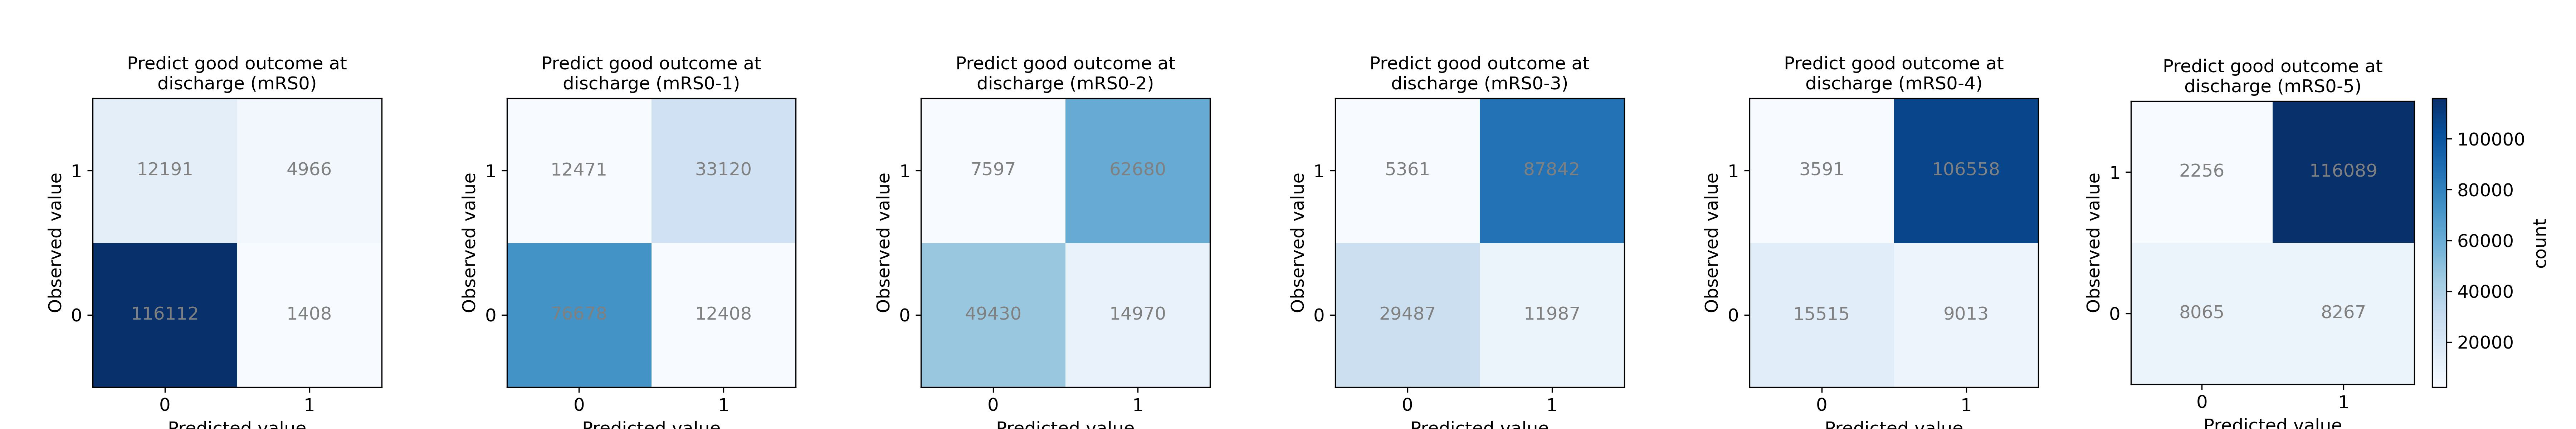
\includegraphics[width=1\textwidth]{./images/073_xgb_all_features_5fold_binary_confusion_matrices_per_binary_threshold_kfold0}\\
      \caption{Kfold 1}
      \label{fig:results_waterfall}
    \end{subfigure}
    \hfill
    \begin{subfigure}[b]{1\textwidth}
      \centering    
      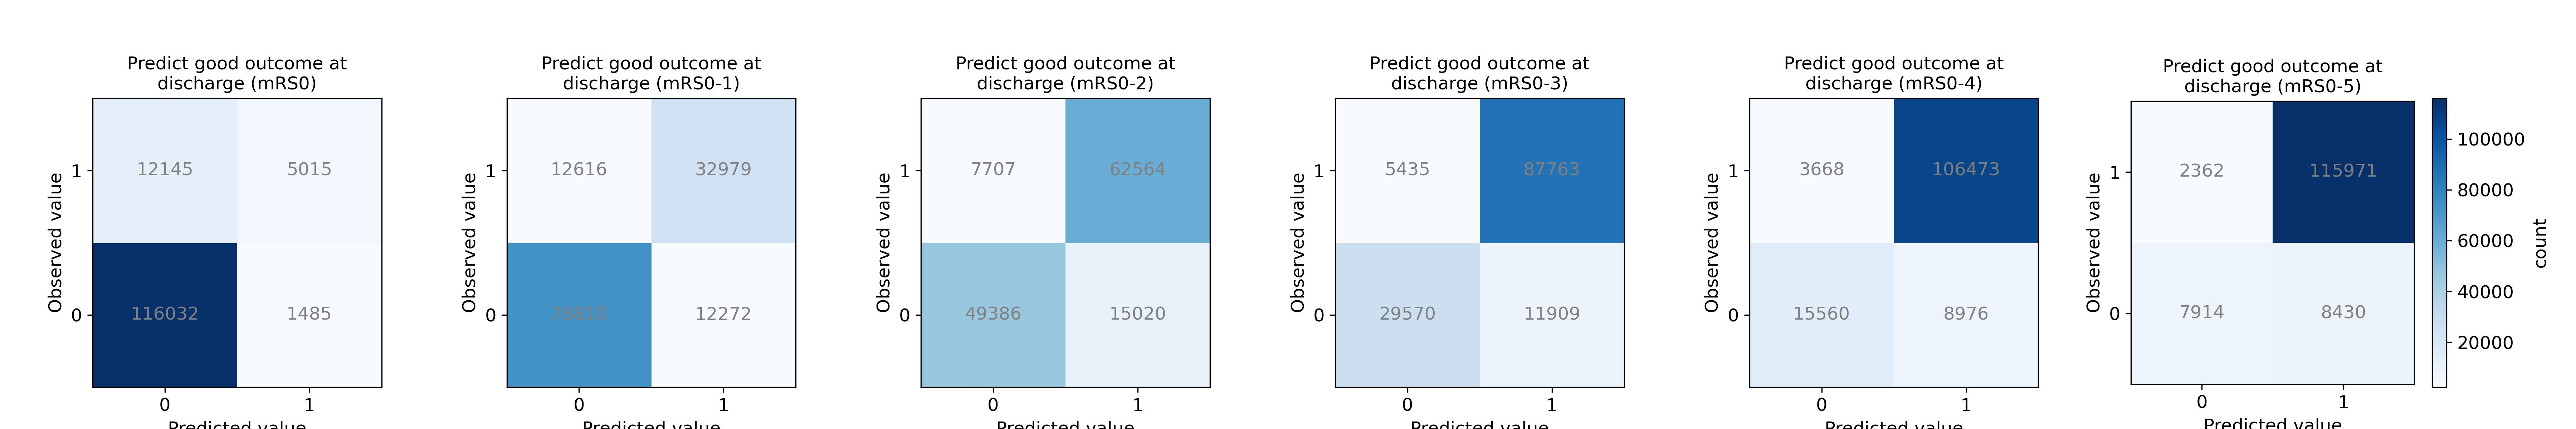
\includegraphics[width=1\textwidth]{./images/073_xgb_all_features_5fold_binary_confusion_matrices_per_binary_threshold_kfold1}\\
      \caption{Kfold 2}
      \label{fig:results_waterfall}
    \end{subfigure}
    \hfill
    \begin{subfigure}[b]{1\textwidth}
      \centering
      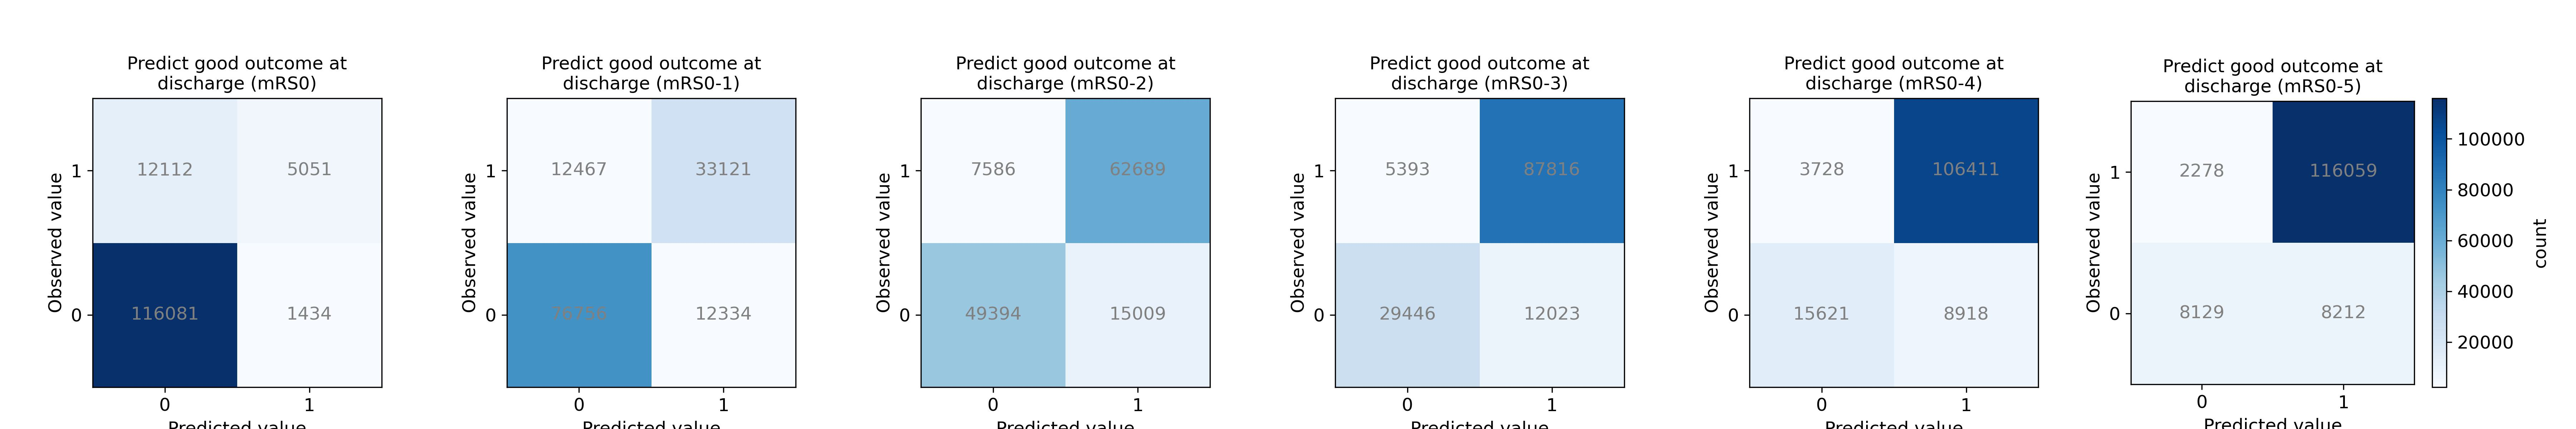
\includegraphics[width=1\textwidth]{./images/073_xgb_all_features_5fold_binary_confusion_matrices_per_binary_threshold_kfold2}\\
      \caption{Kfold 3}
      \label{fig:results_waterfall}
    \end{subfigure}
    \hfill
    \begin{subfigure}[b]{1\textwidth}
      \centering
      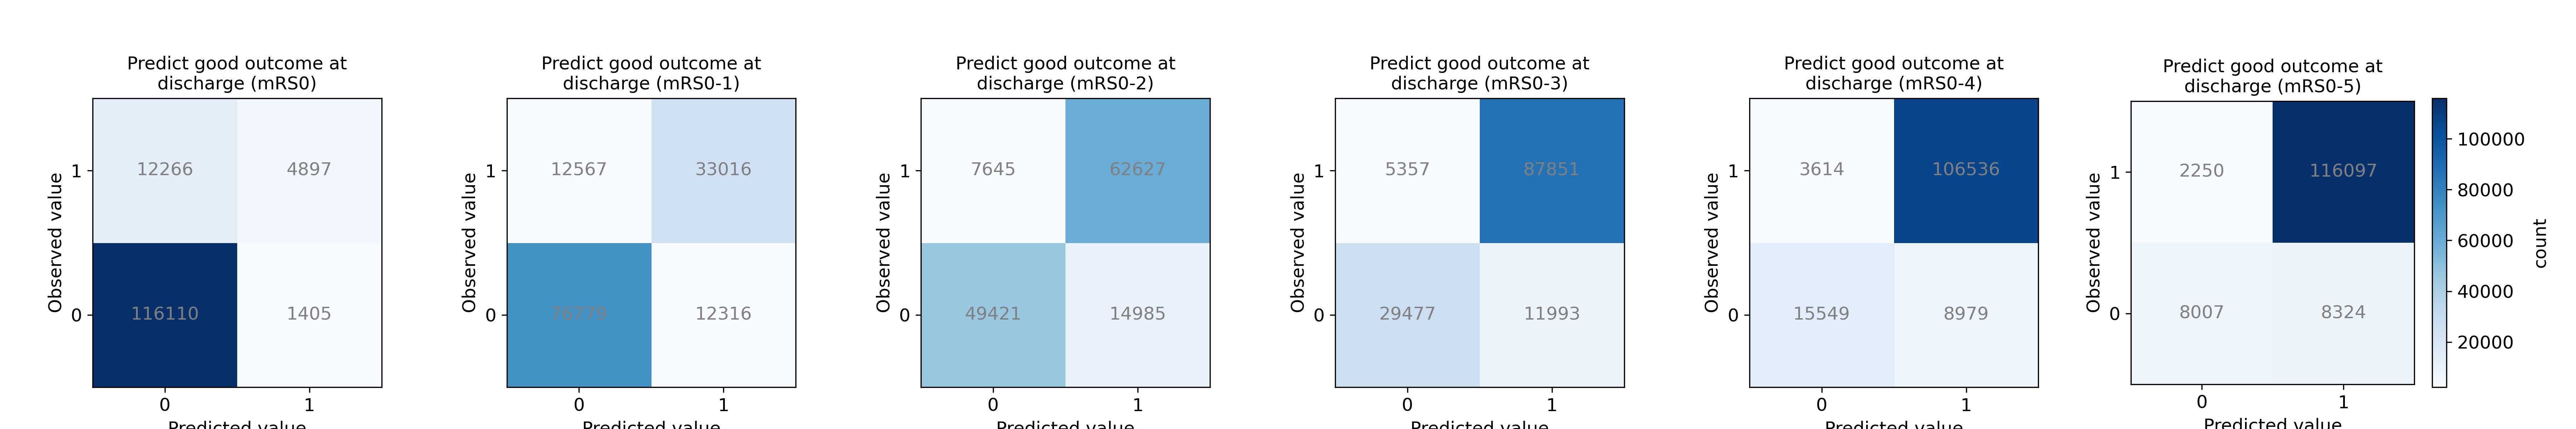
\includegraphics[width=1\textwidth]{./images/073_xgb_all_features_5fold_binary_confusion_matrices_per_binary_threshold_kfold3}\\
      \caption{Kfold 4}
      \label{fig:results_waterfall}
    \end{subfigure}
    \hfill
    \begin{subfigure}[b]{1\textwidth}
      \centering
      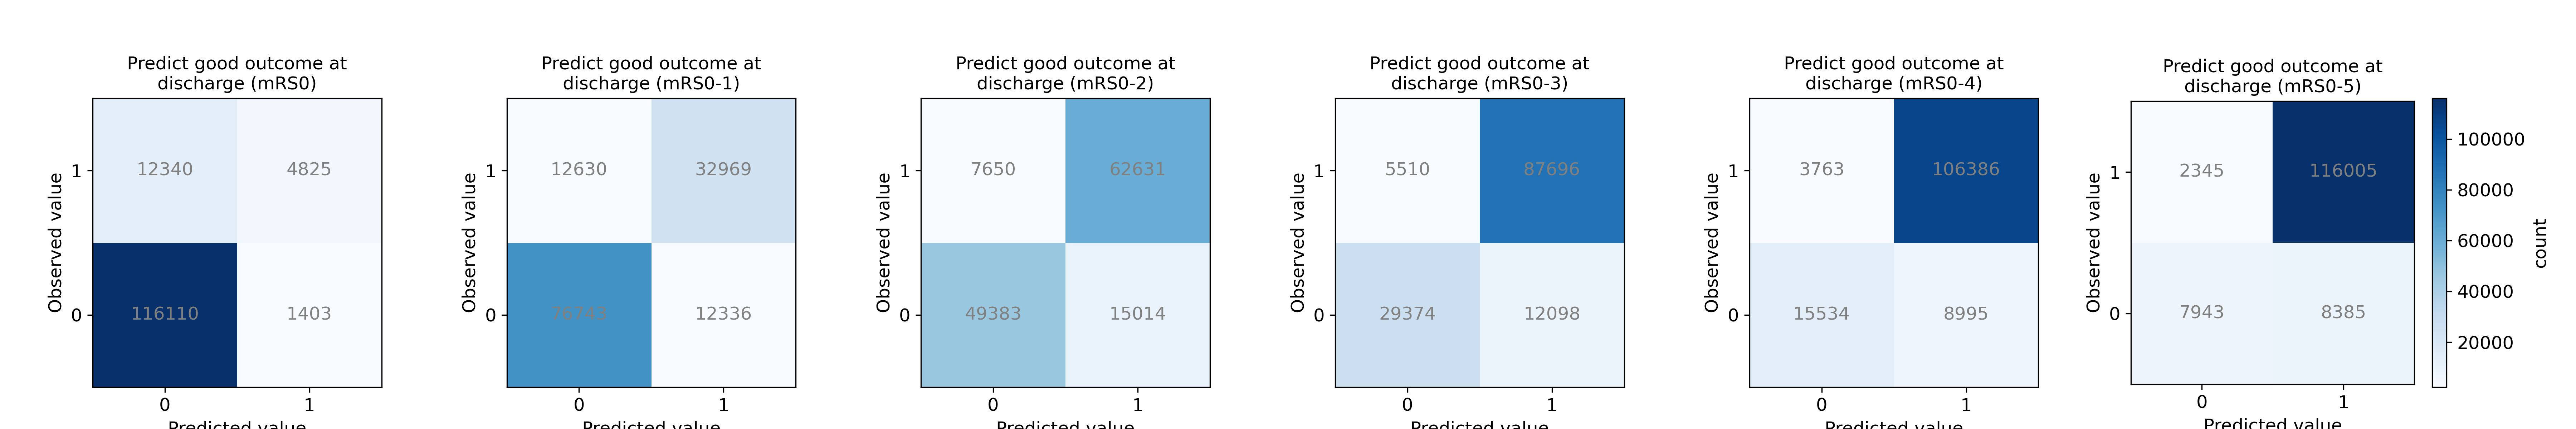
\includegraphics[width=1\textwidth]{./images/073_xgb_all_features_5fold_binary_confusion_matrices_per_binary_threshold_kfold4}\\
      \caption{Kfold 5}
      \label{fig:results_waterfall}
    \end{subfigure}
  \caption{Confusion matrices for each kfold (model with all features)}
\end{figure}

\begin{figure}[!ht]
\centering
    \subfloat[]{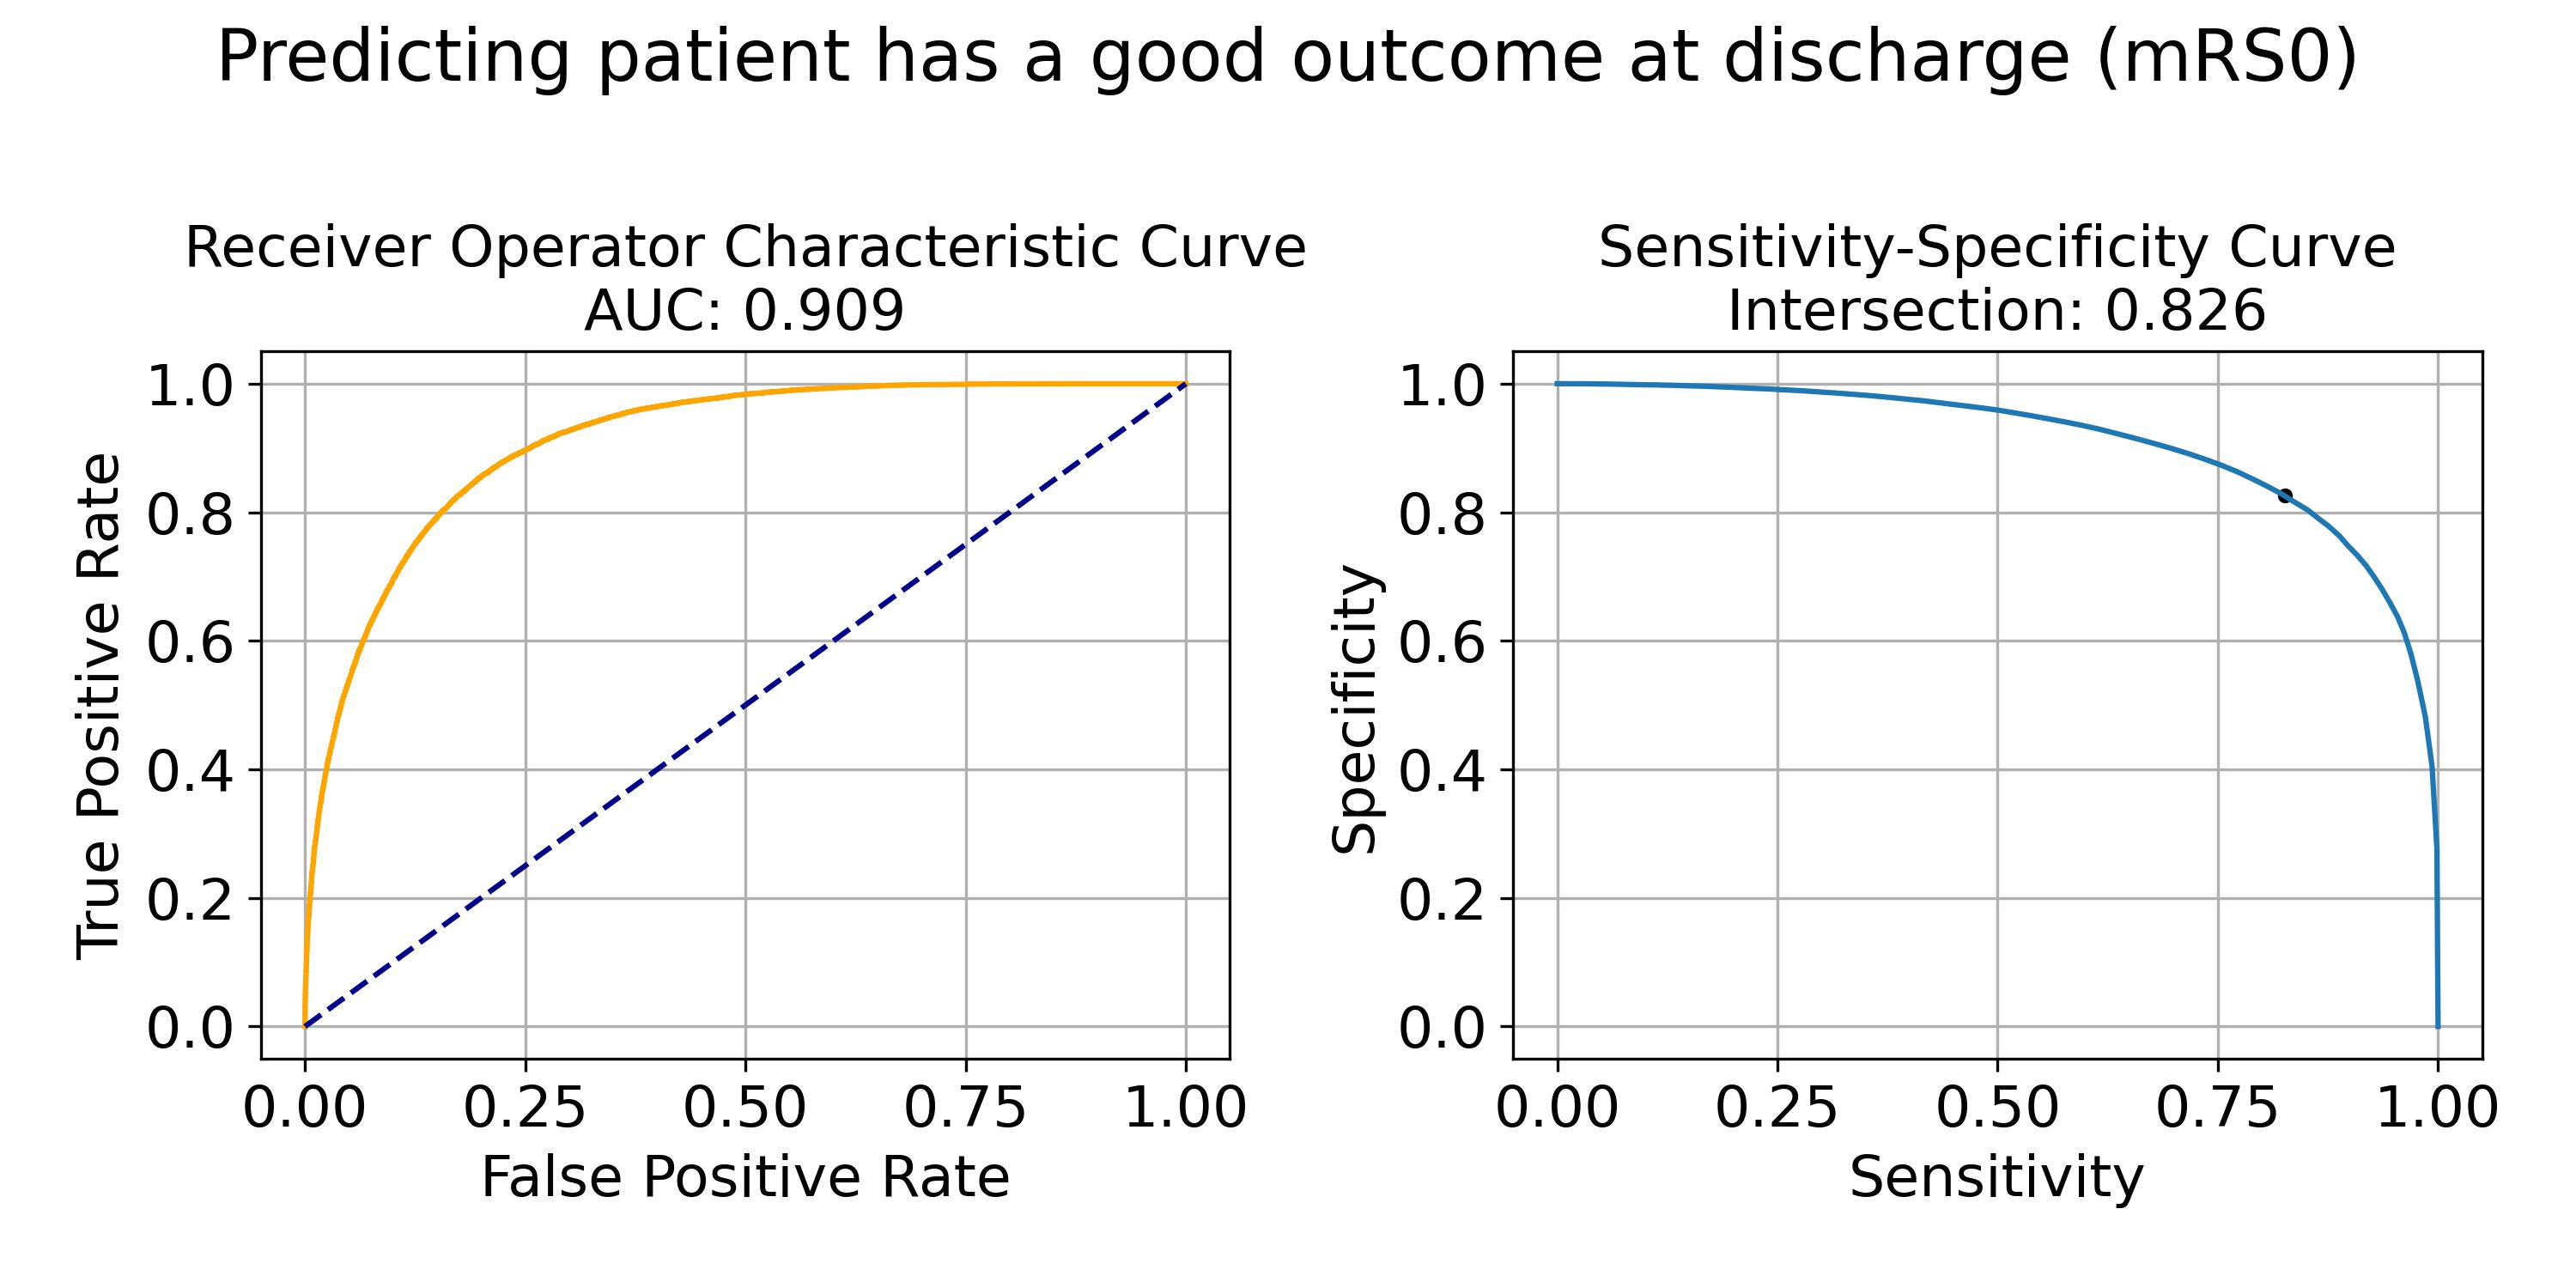
\includegraphics[width=0.5\linewidth]{./images/073_xgb_all_features_5fold_binary_roc_sens_spec_mrs0_kfold0_paper}}
\hfil
    \subfloat[]{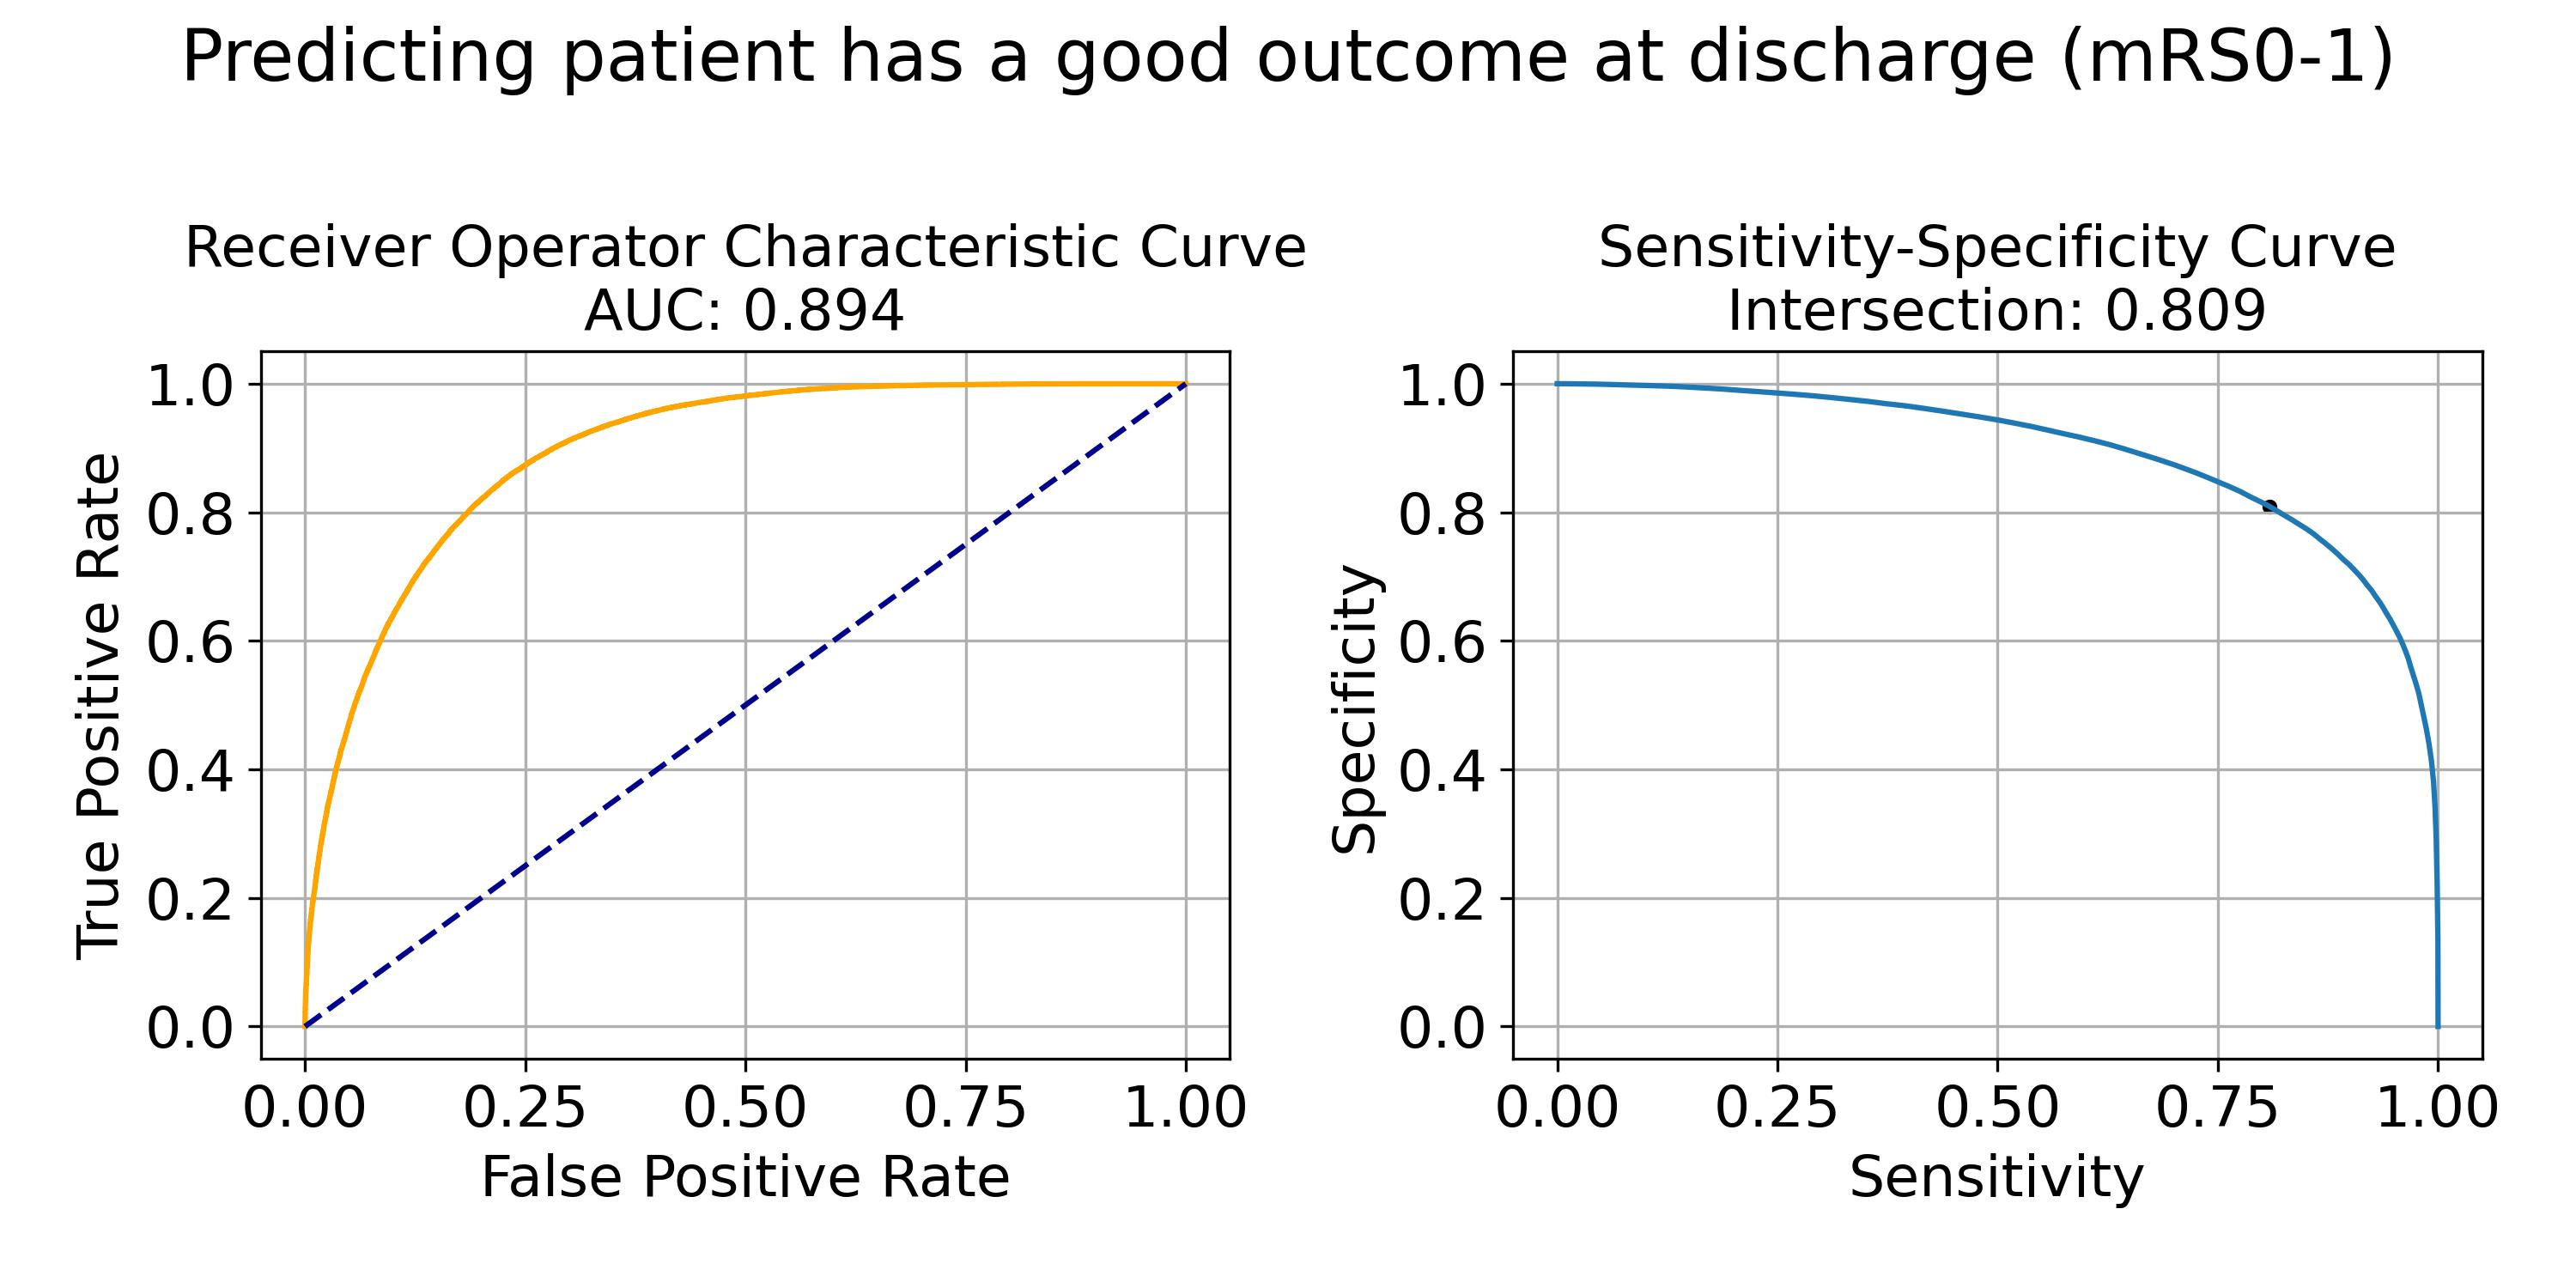
\includegraphics[width=0.5\linewidth]{./images/073_xgb_all_features_5fold_binary_roc_sens_spec_mrs1_kfold0_paper}}

    \subfloat[]{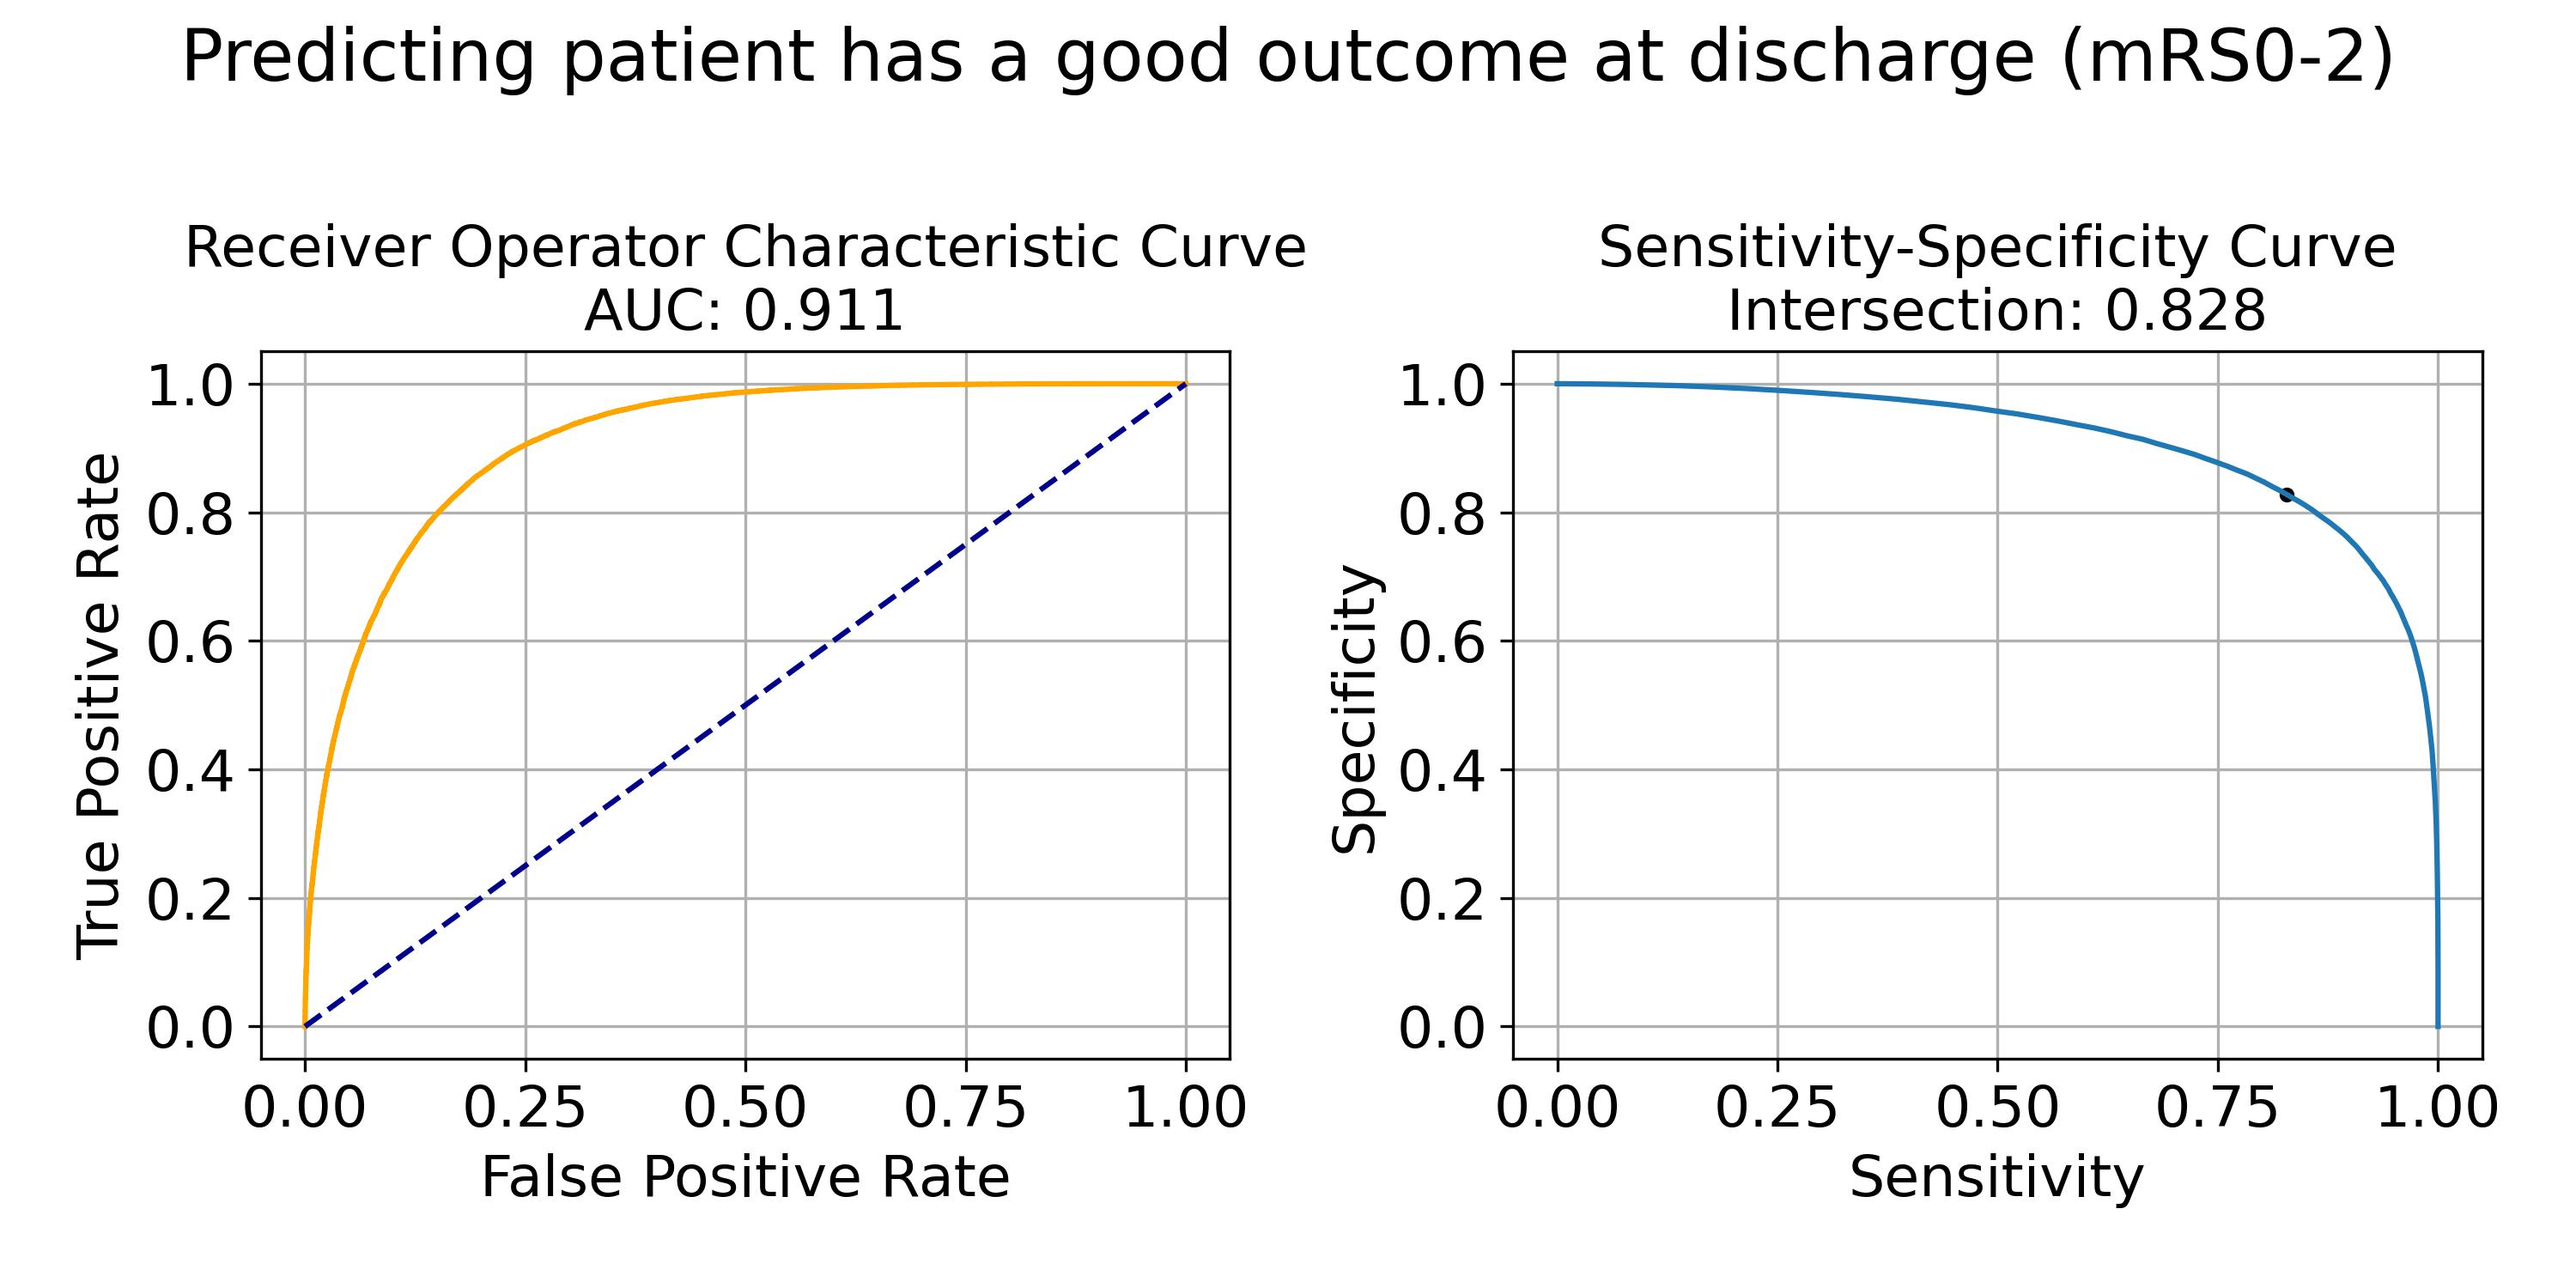
\includegraphics[width=0.5\linewidth]{./images/073_xgb_all_features_5fold_binary_roc_sens_spec_mrs2_kfold0_paper}}
\hfil
    \subfloat[]{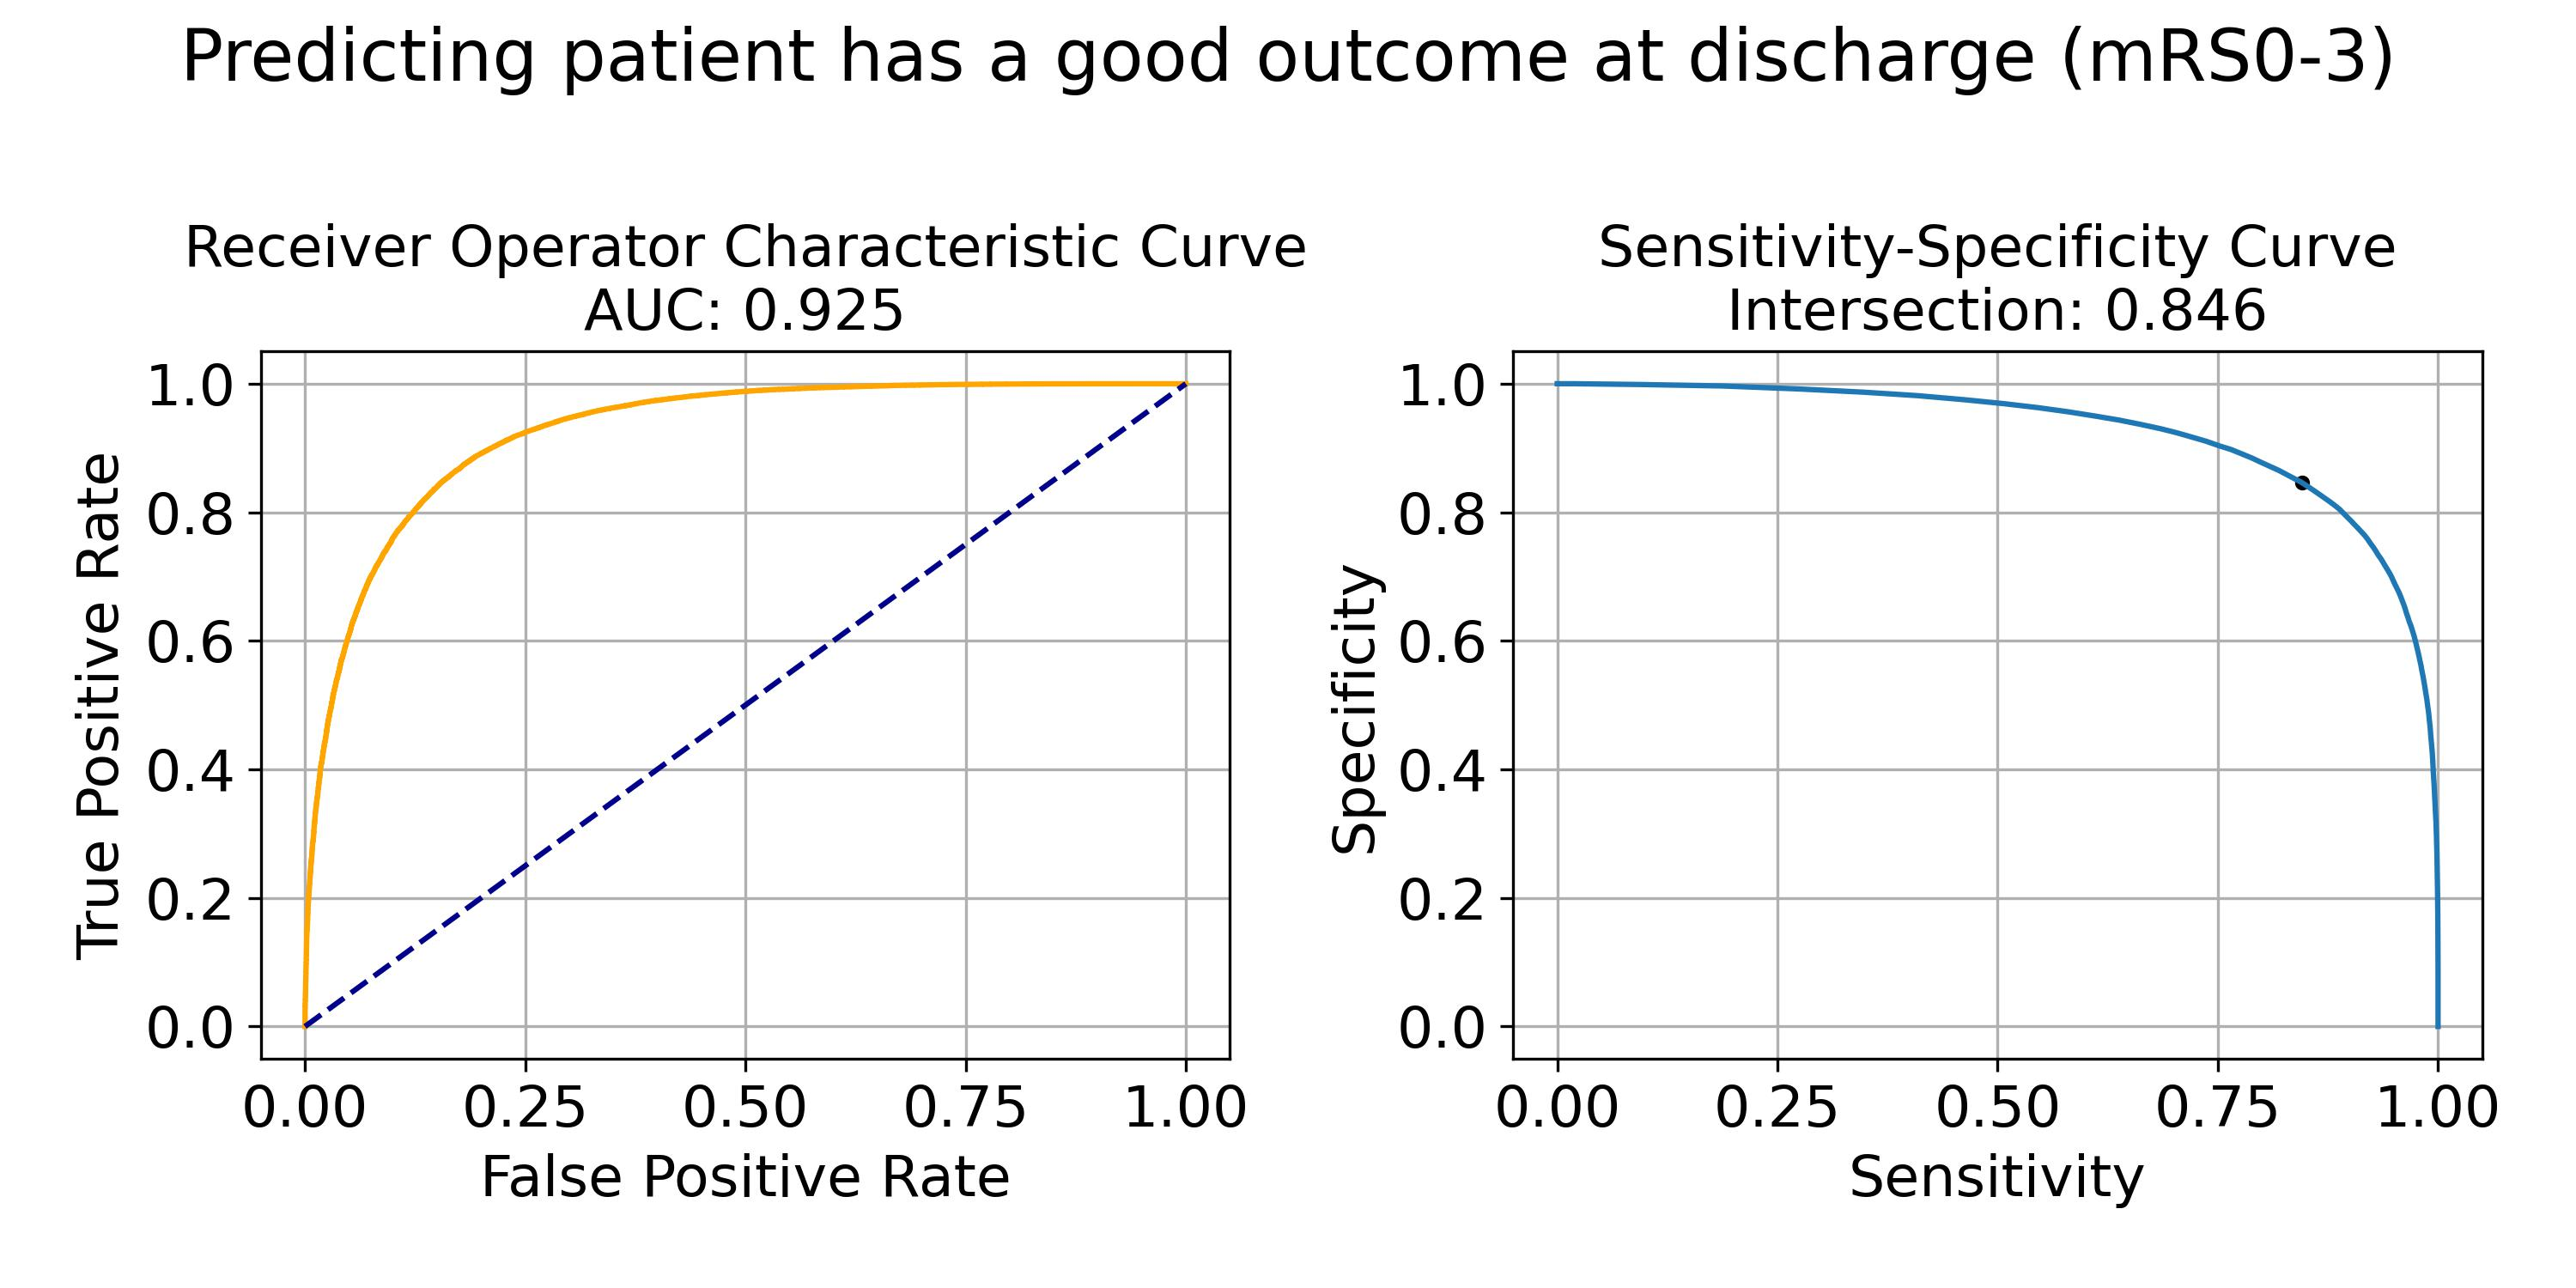
\includegraphics[width=0.5\linewidth]{./images/073_xgb_all_features_5fold_binary_roc_sens_spec_mrs3_kfold0_paper}}

    \subfloat[]{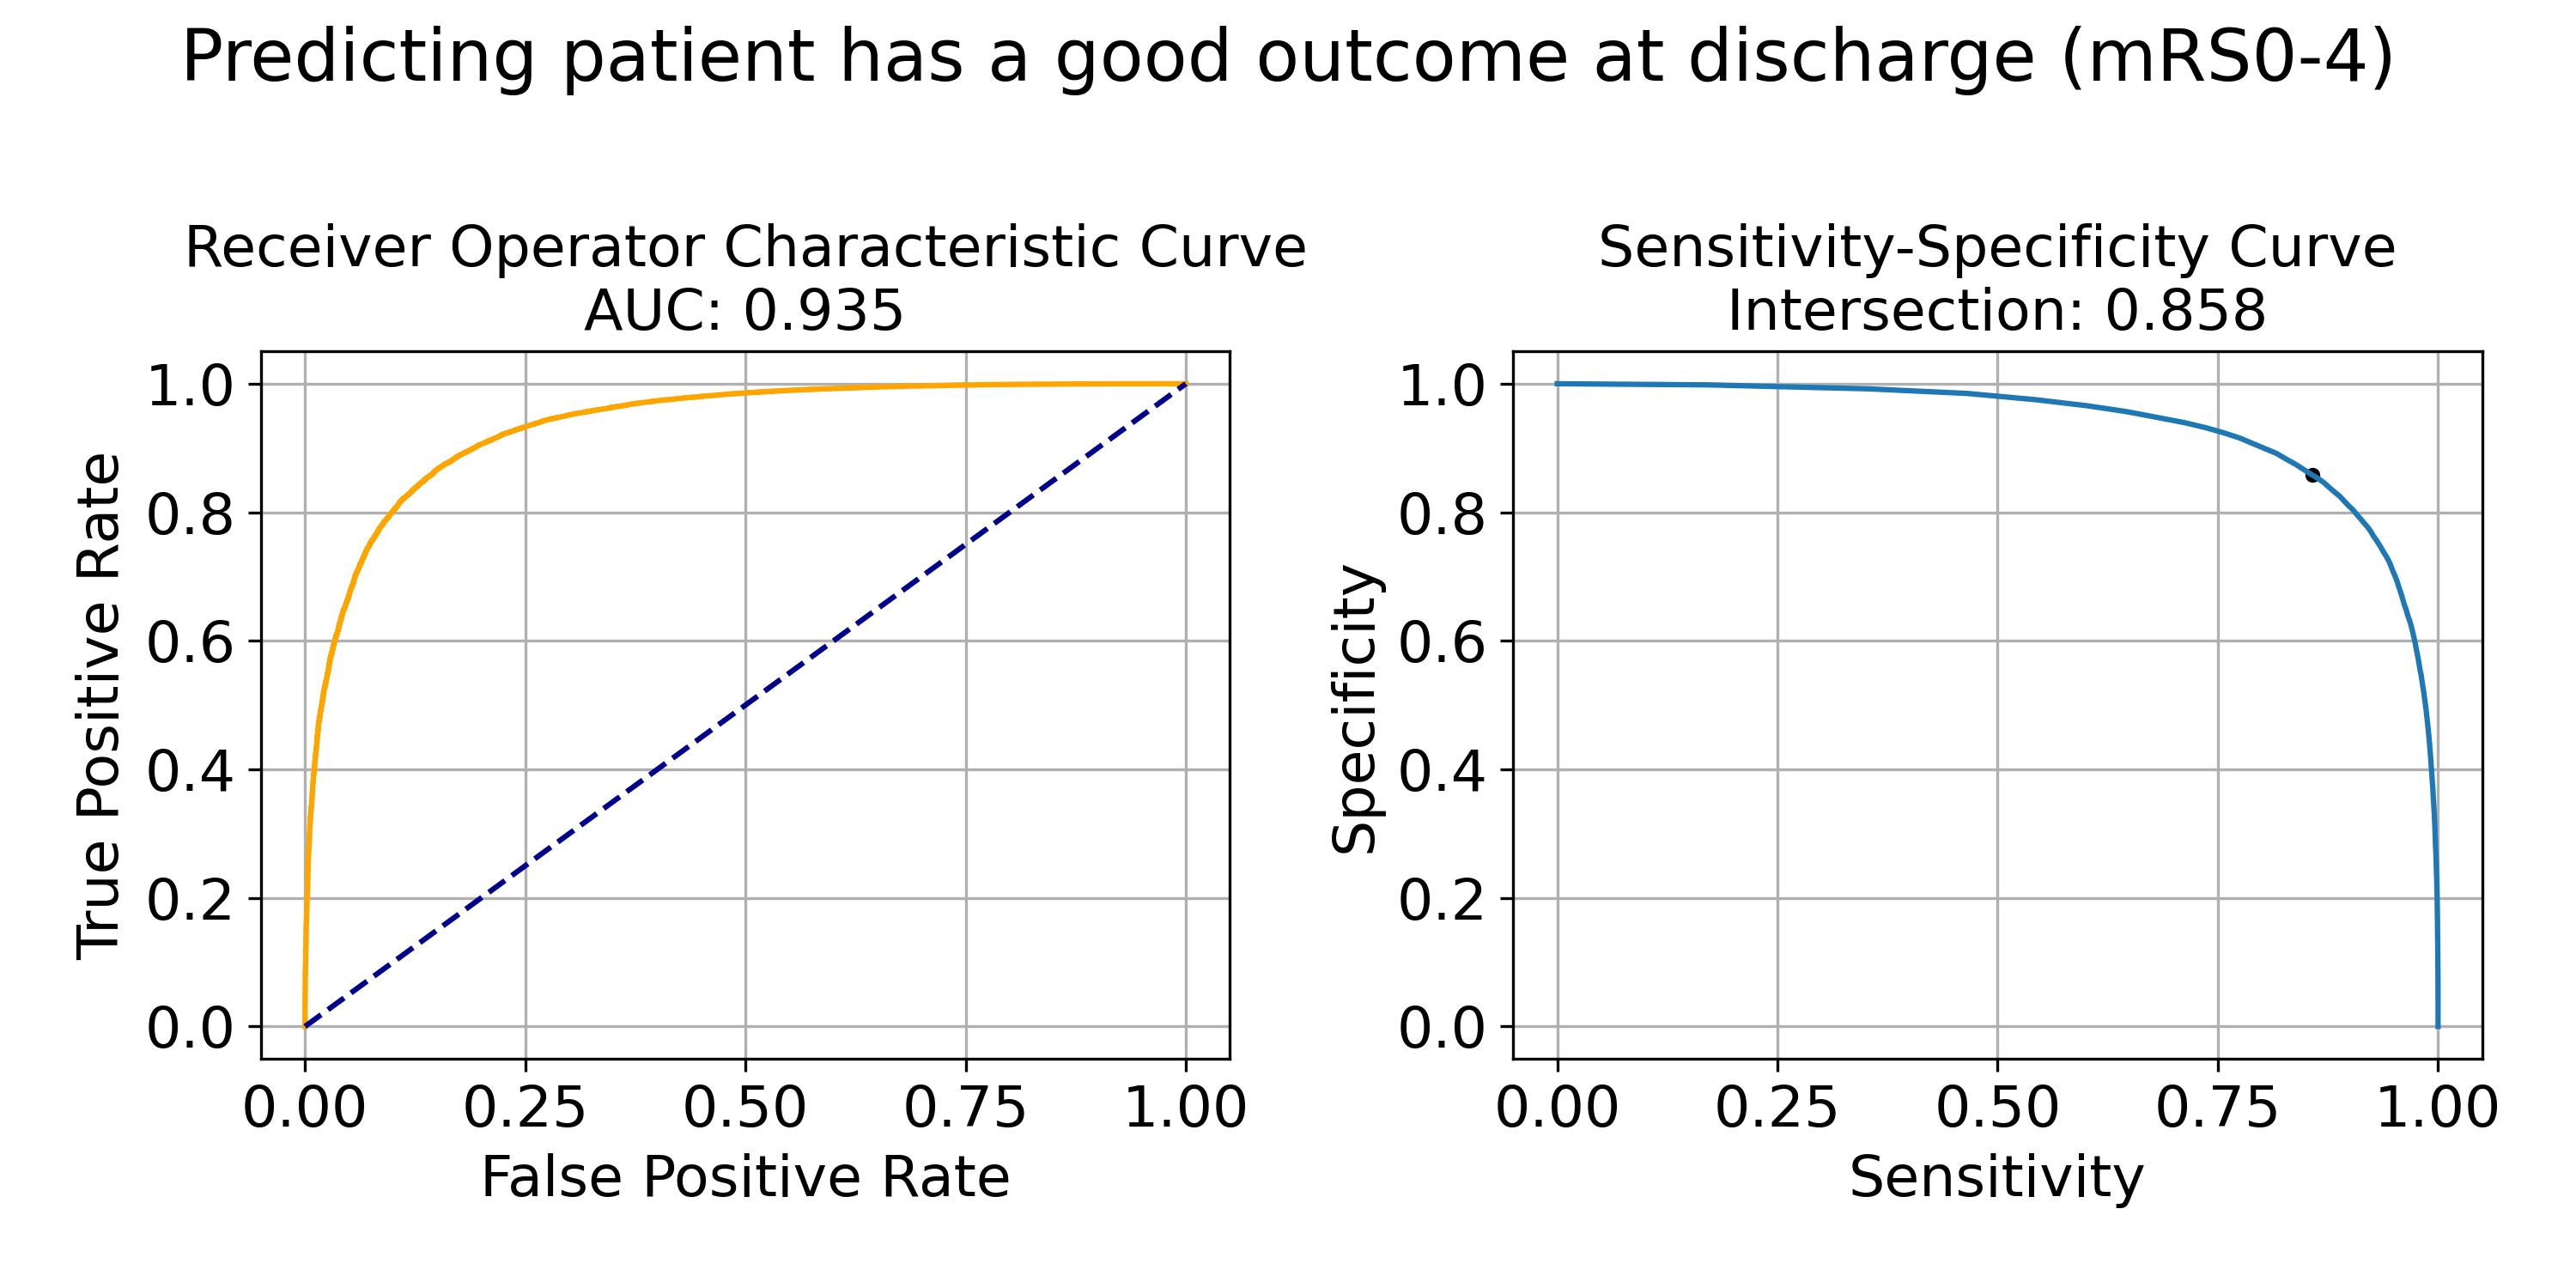
\includegraphics[width=0.5\linewidth]{./images/073_xgb_all_features_5fold_binary_roc_sens_spec_mrs4_kfold0_paper}}
\hfil
    \subfloat[]{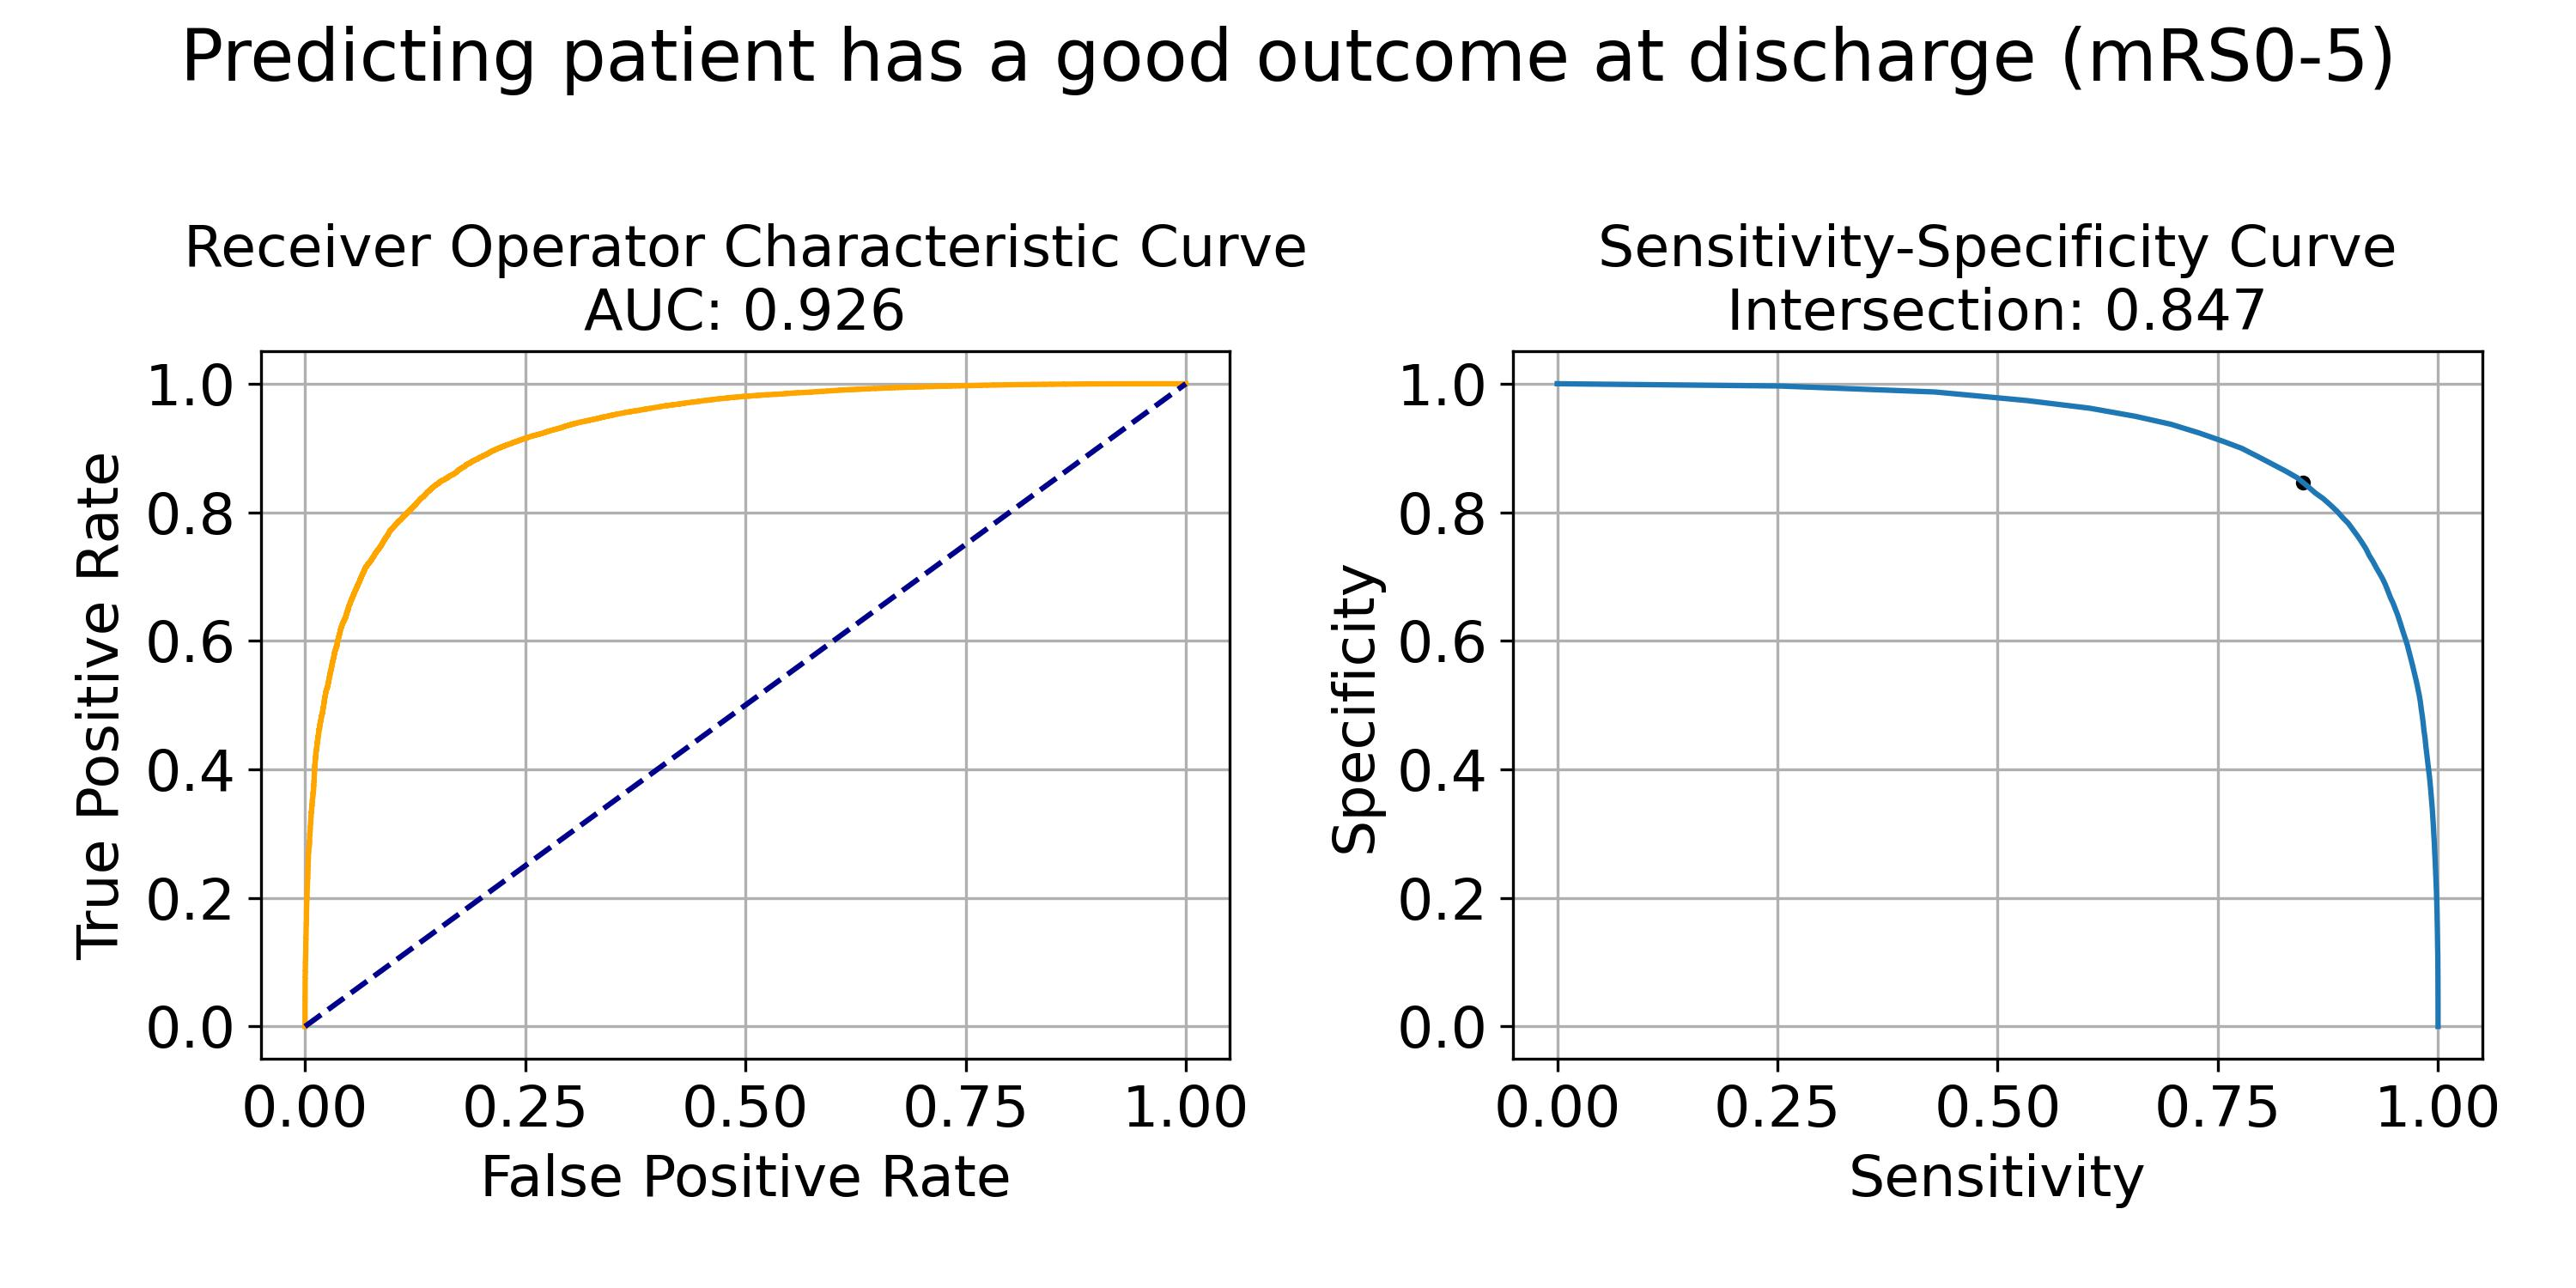
\includegraphics[width=0.5\linewidth]{./images/073_xgb_all_features_5fold_binary_roc_sens_spec_mrs5_kfold0_paper}}
    \label{fig:rocauc_ss_all_features}
  \caption{ROC AUC, and specificity and sensitivity plots for each of the mRS threshold levels to define a good outcome (for first kfold). All features as model inputs.}

\end{figure}






\subsection{Model accuracy}


Figure \ref{fig:feature_selection} shows the mean ROCAUC for the 5 kfold model, sequentially selecting the features.

\begin{figure}[!h]
    \centering
    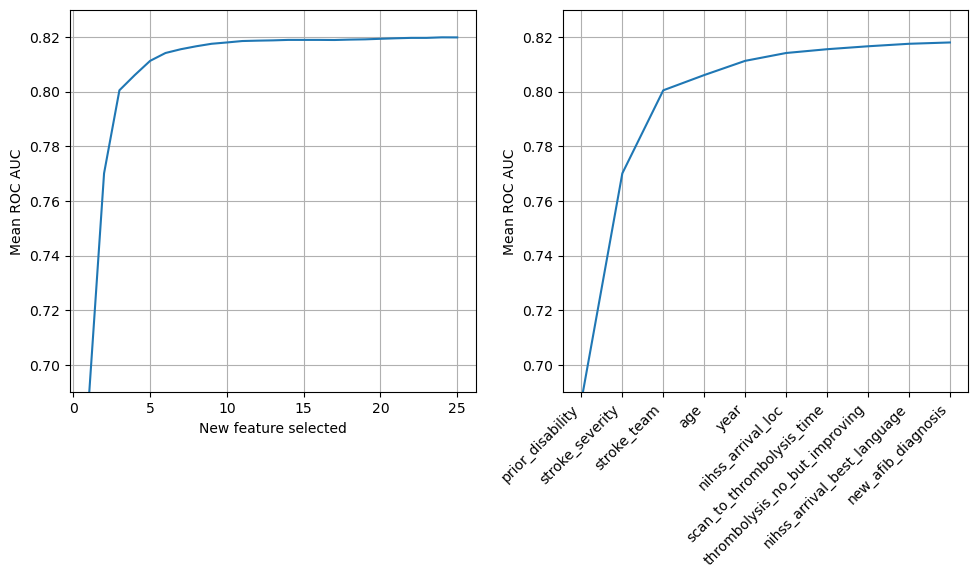
\includegraphics[width=0.75\textwidth]{./images/020_feature_selection.jpg}\\
    \caption{Feature selection}
    \label{fig:feature_selection}
\end{figure}

{ROCAUC}

Figure \ref{fig:confusion_rocauc} shows the ROCAUC results for the individual one vs one classes. There is a better performance for classes to be distiguishable when they are further from each other in value. 

\begin{figure}
    \centering
    {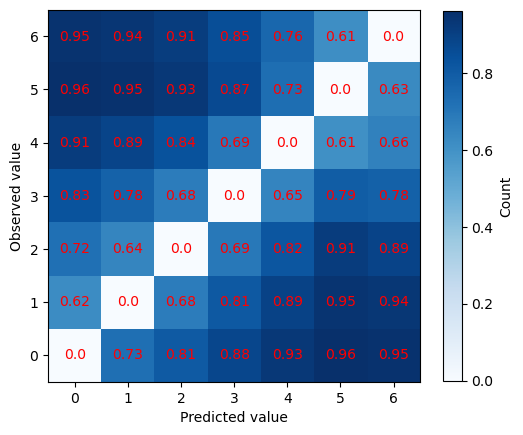
\includegraphics[width = 4in]{./images/040_ROCAUC_confusion_matrix_ovo.png}}\\
    \caption{}
    \label{fig:confusion_rocauc}
\end{figure}

Figure \ref{fig:confusion_mrs} shows the confusion matrices for the 5 kfolds. Given the consistency across the 5 kfolds, we will now only use results from the first kfold.

\begin{figure}[!h]
    \centering
    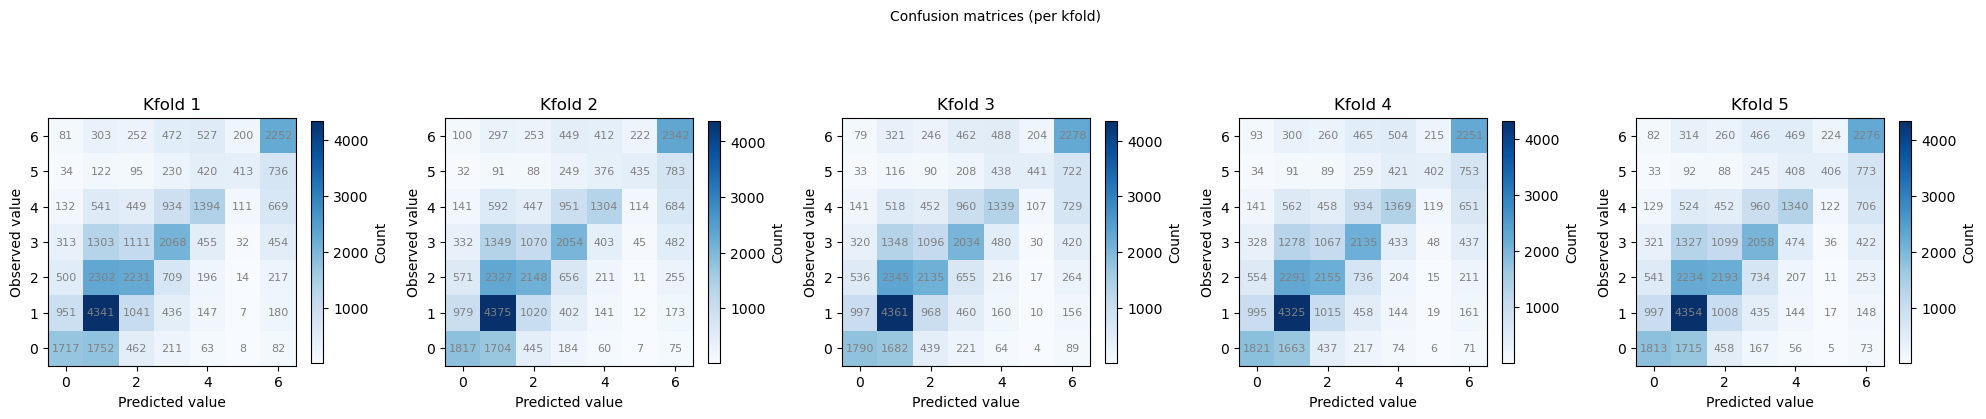
\includegraphics[trim={0 0 0 1.2cm}, clip, width=1\textwidth]{./images/040_confusion_matrices_5fold.png}\\
    \caption{}
    \label{fig:confusion_mrs}
\end{figure}


\section{Method}

\subsection{Data}

Data were retrieved for 168,347 emergency stroke admissions to acute stroke teams in England for six years, 2016–2021 (inclusive), obtained from the Sentinel Stroke National Audit Programme (SSNAP). Data fields were provided for the hyper-acute phase of the stroke pathway, up to and including our target feature: disability on inpatient discharge. Disability is recorded in the SSNAP dataset using the modified Rankin Scale (mRS), where mRS 0 represents perfect health and mRS 6 represents death. The data includes 118 acute stroke hospitals (each has at least 250 stroke admissions and delivers thrombolysis to at least 10 patients in the six years).

\subsection{Machine learning models}

\subsection{Model accuracy}

\begin{figure}[!h]
    \centering
    \begin{subfigure}[b]{1\textwidth}
      \centering
      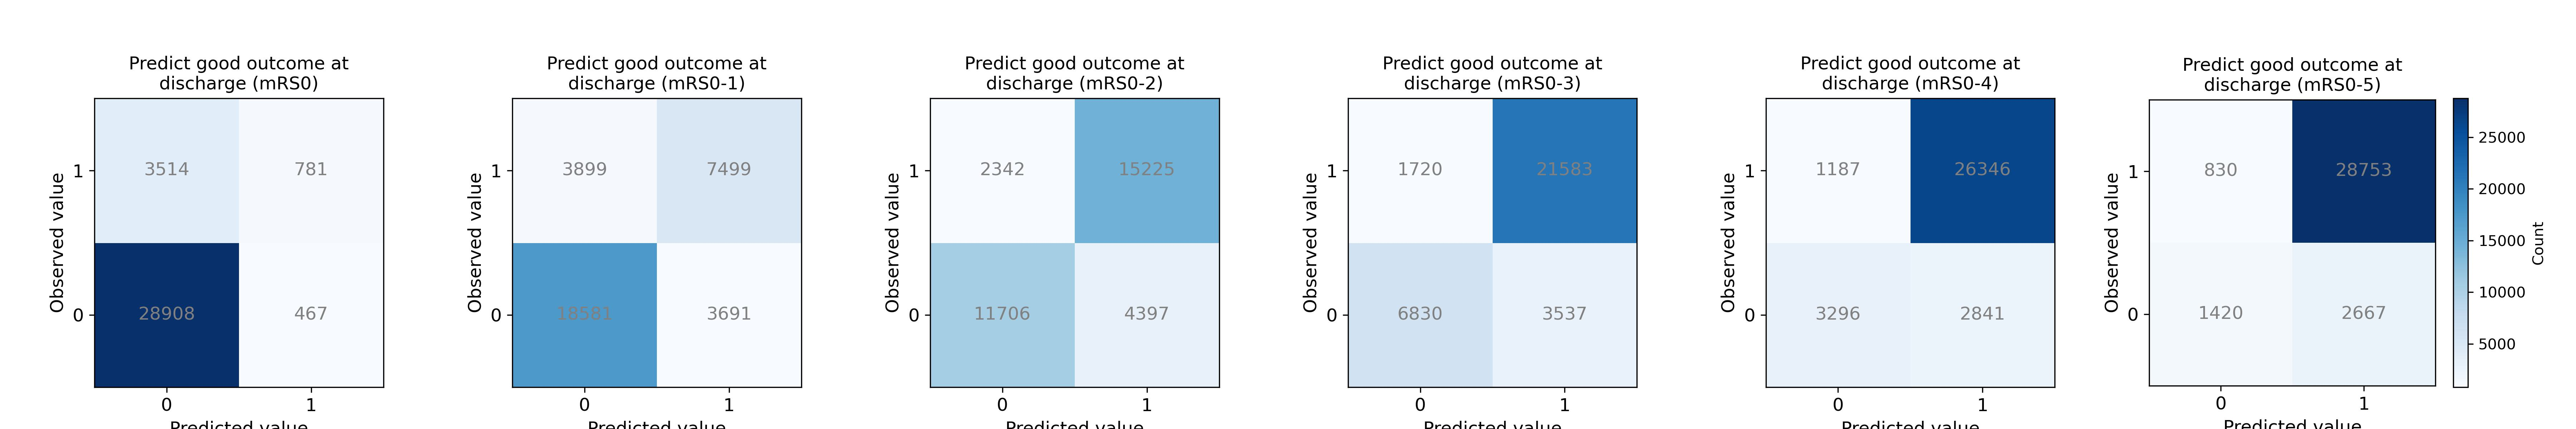
\includegraphics[width=1\textwidth]{./images/083_xgb_7_features_5fold_binary_confusion_matrices_per_binary_threshold_kfold0}\\
      \caption{Kfold 1}
      \label{fig:results_waterfall}
    \end{subfigure}
    \hfill
    \begin{subfigure}[b]{1\textwidth}
      \centering    
      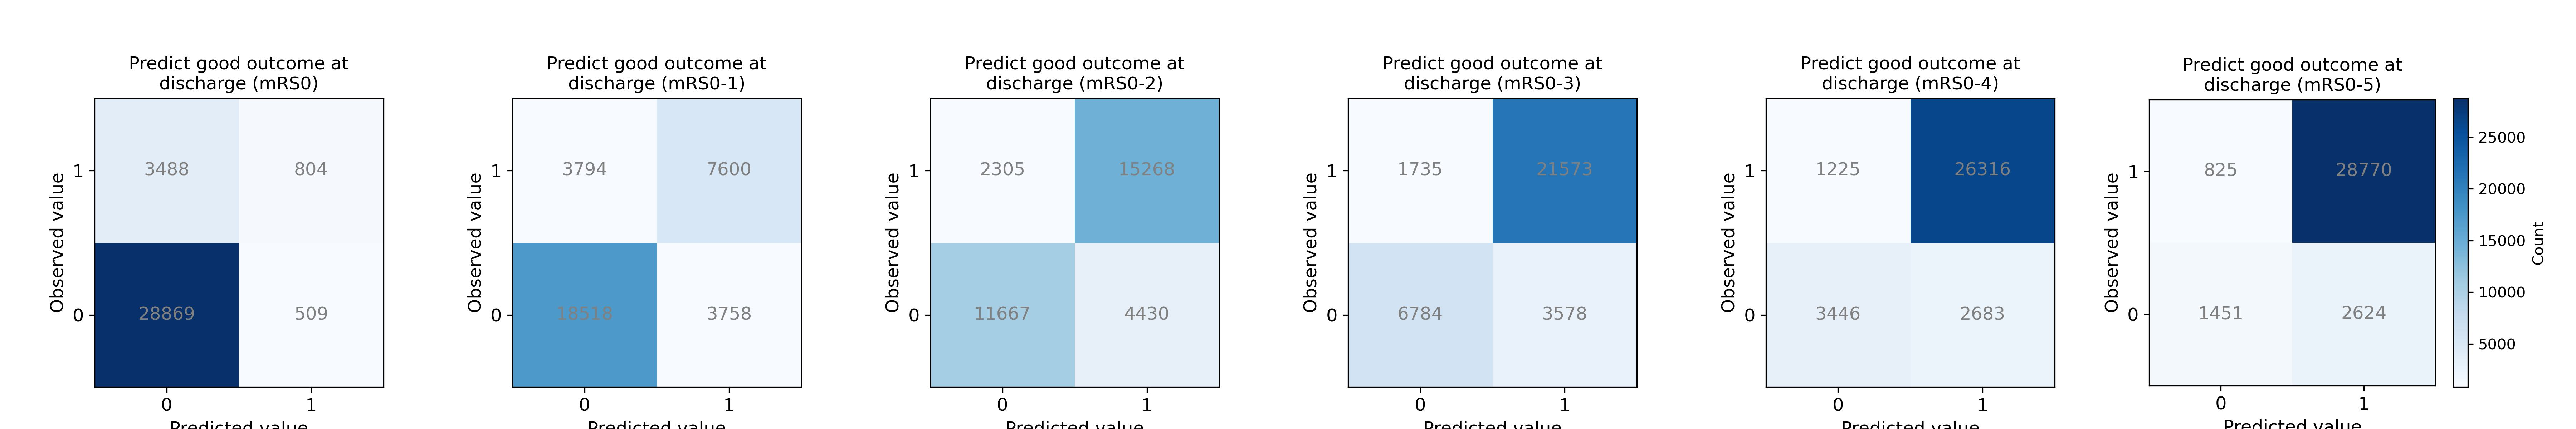
\includegraphics[width=1\textwidth]{./images/083_xgb_7_features_5fold_binary_confusion_matrices_per_binary_threshold_kfold1}\\
      \caption{Kfold 2}
      \label{fig:results_waterfall}
    \end{subfigure}
    \hfill
    \begin{subfigure}[b]{1\textwidth}
      \centering
      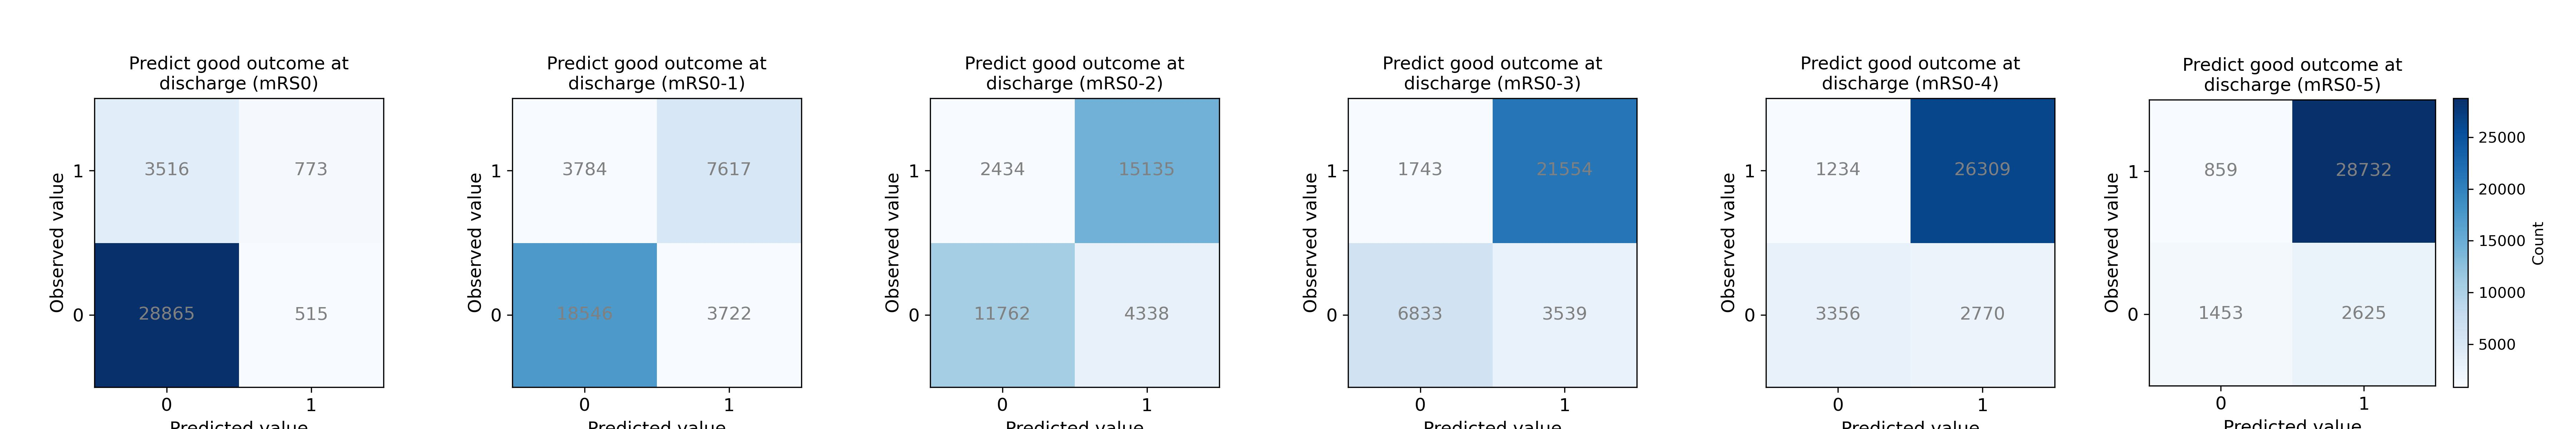
\includegraphics[width=1\textwidth]{./images/083_xgb_7_features_5fold_binary_confusion_matrices_per_binary_threshold_kfold2}\\
      \caption{Kfold 3}
      \label{fig:results_waterfall}
    \end{subfigure}
    \hfill
    \begin{subfigure}[b]{1\textwidth}
      \centering
      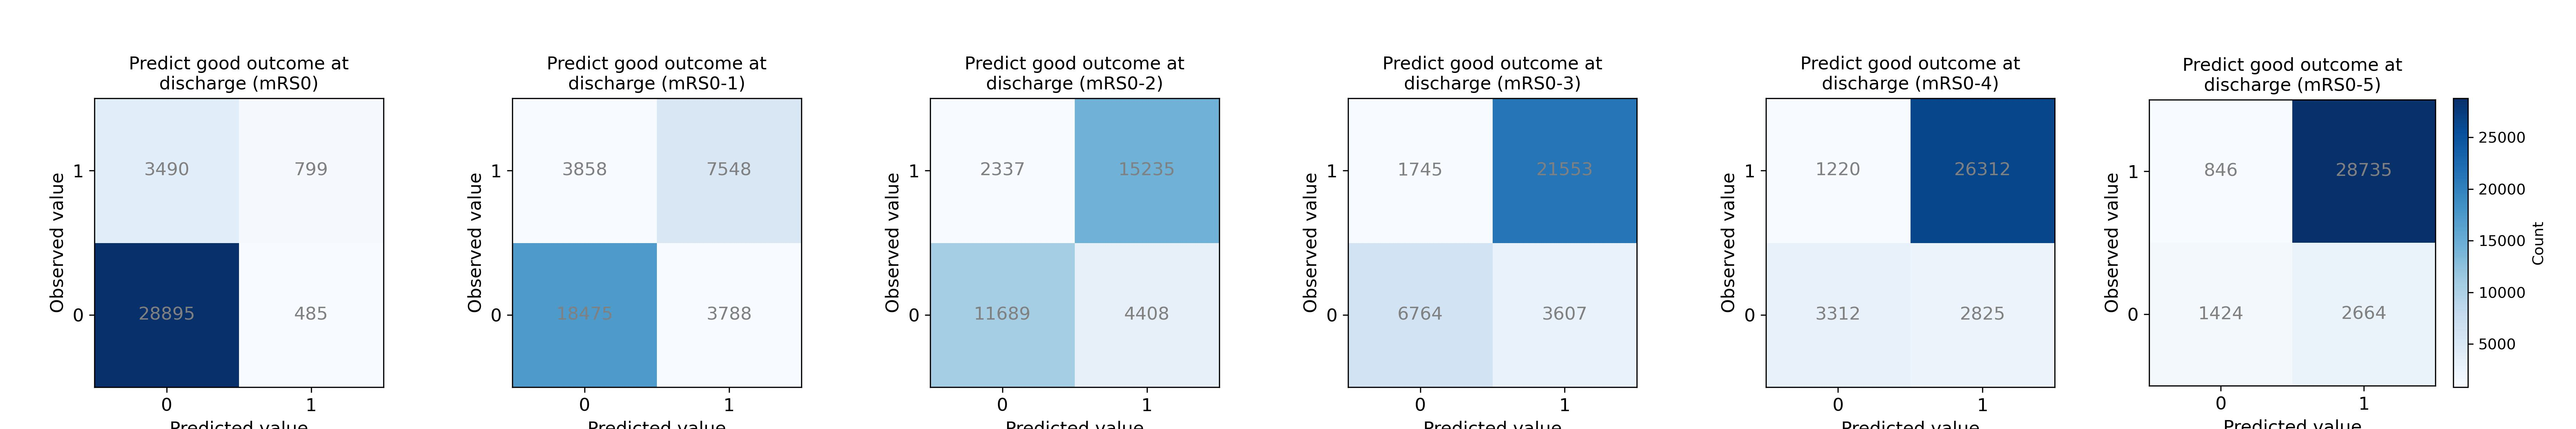
\includegraphics[width=1\textwidth]{./images/083_xgb_7_features_5fold_binary_confusion_matrices_per_binary_threshold_kfold3}\\
      \caption{Kfold 4}
      \label{fig:results_waterfall}
    \end{subfigure}
    \hfill
    \begin{subfigure}[b]{1\textwidth}
      \centering
      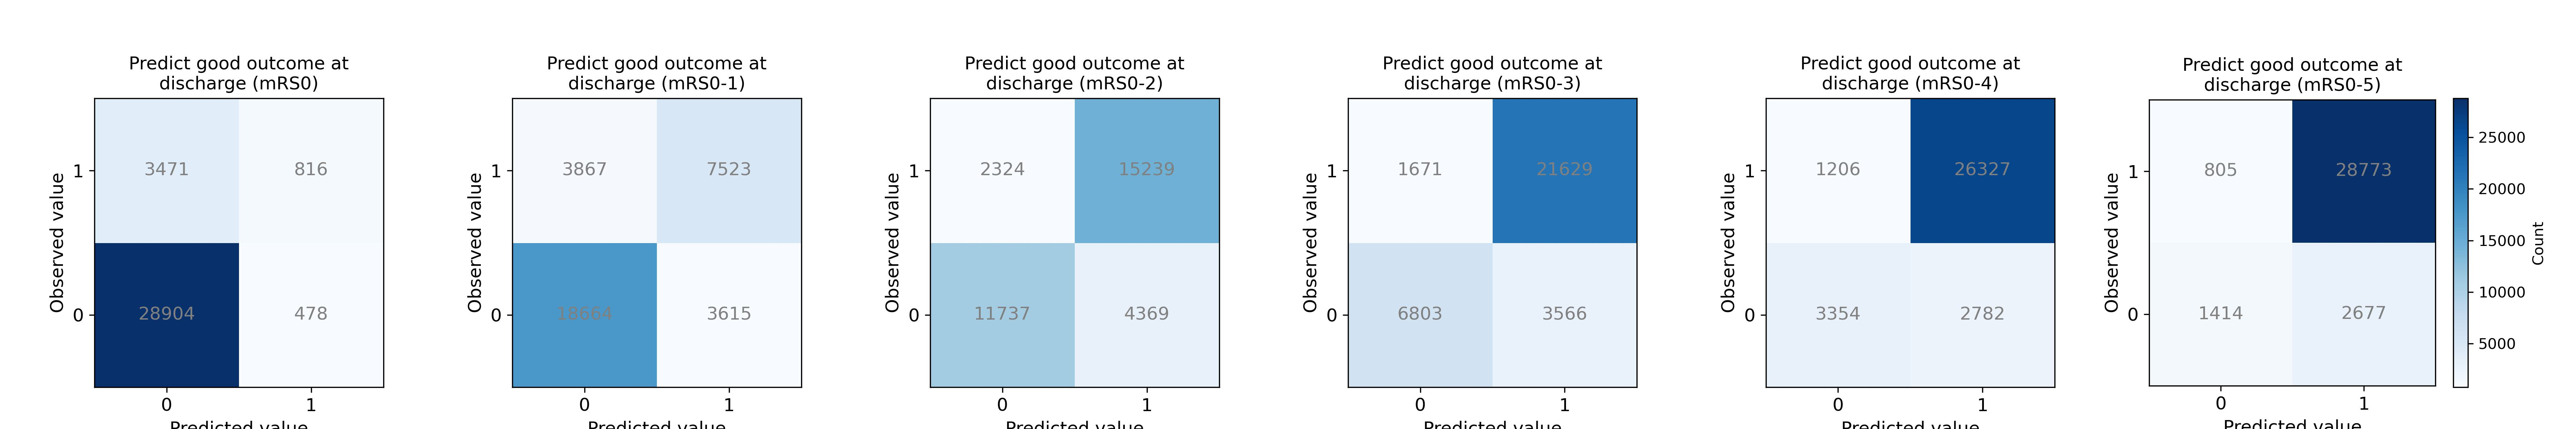
\includegraphics[width=1\textwidth]{./images/083_xgb_7_features_5fold_binary_confusion_matrices_per_binary_threshold_kfold4}\\
      \caption{Kfold 5}
      \label{fig:results_waterfall}
    \end{subfigure}
  \caption{Confusion matrices for each kfold (model with 7 features)}
\end{figure}


\begin{figure}[!ht]
\centering
    \subfloat[]{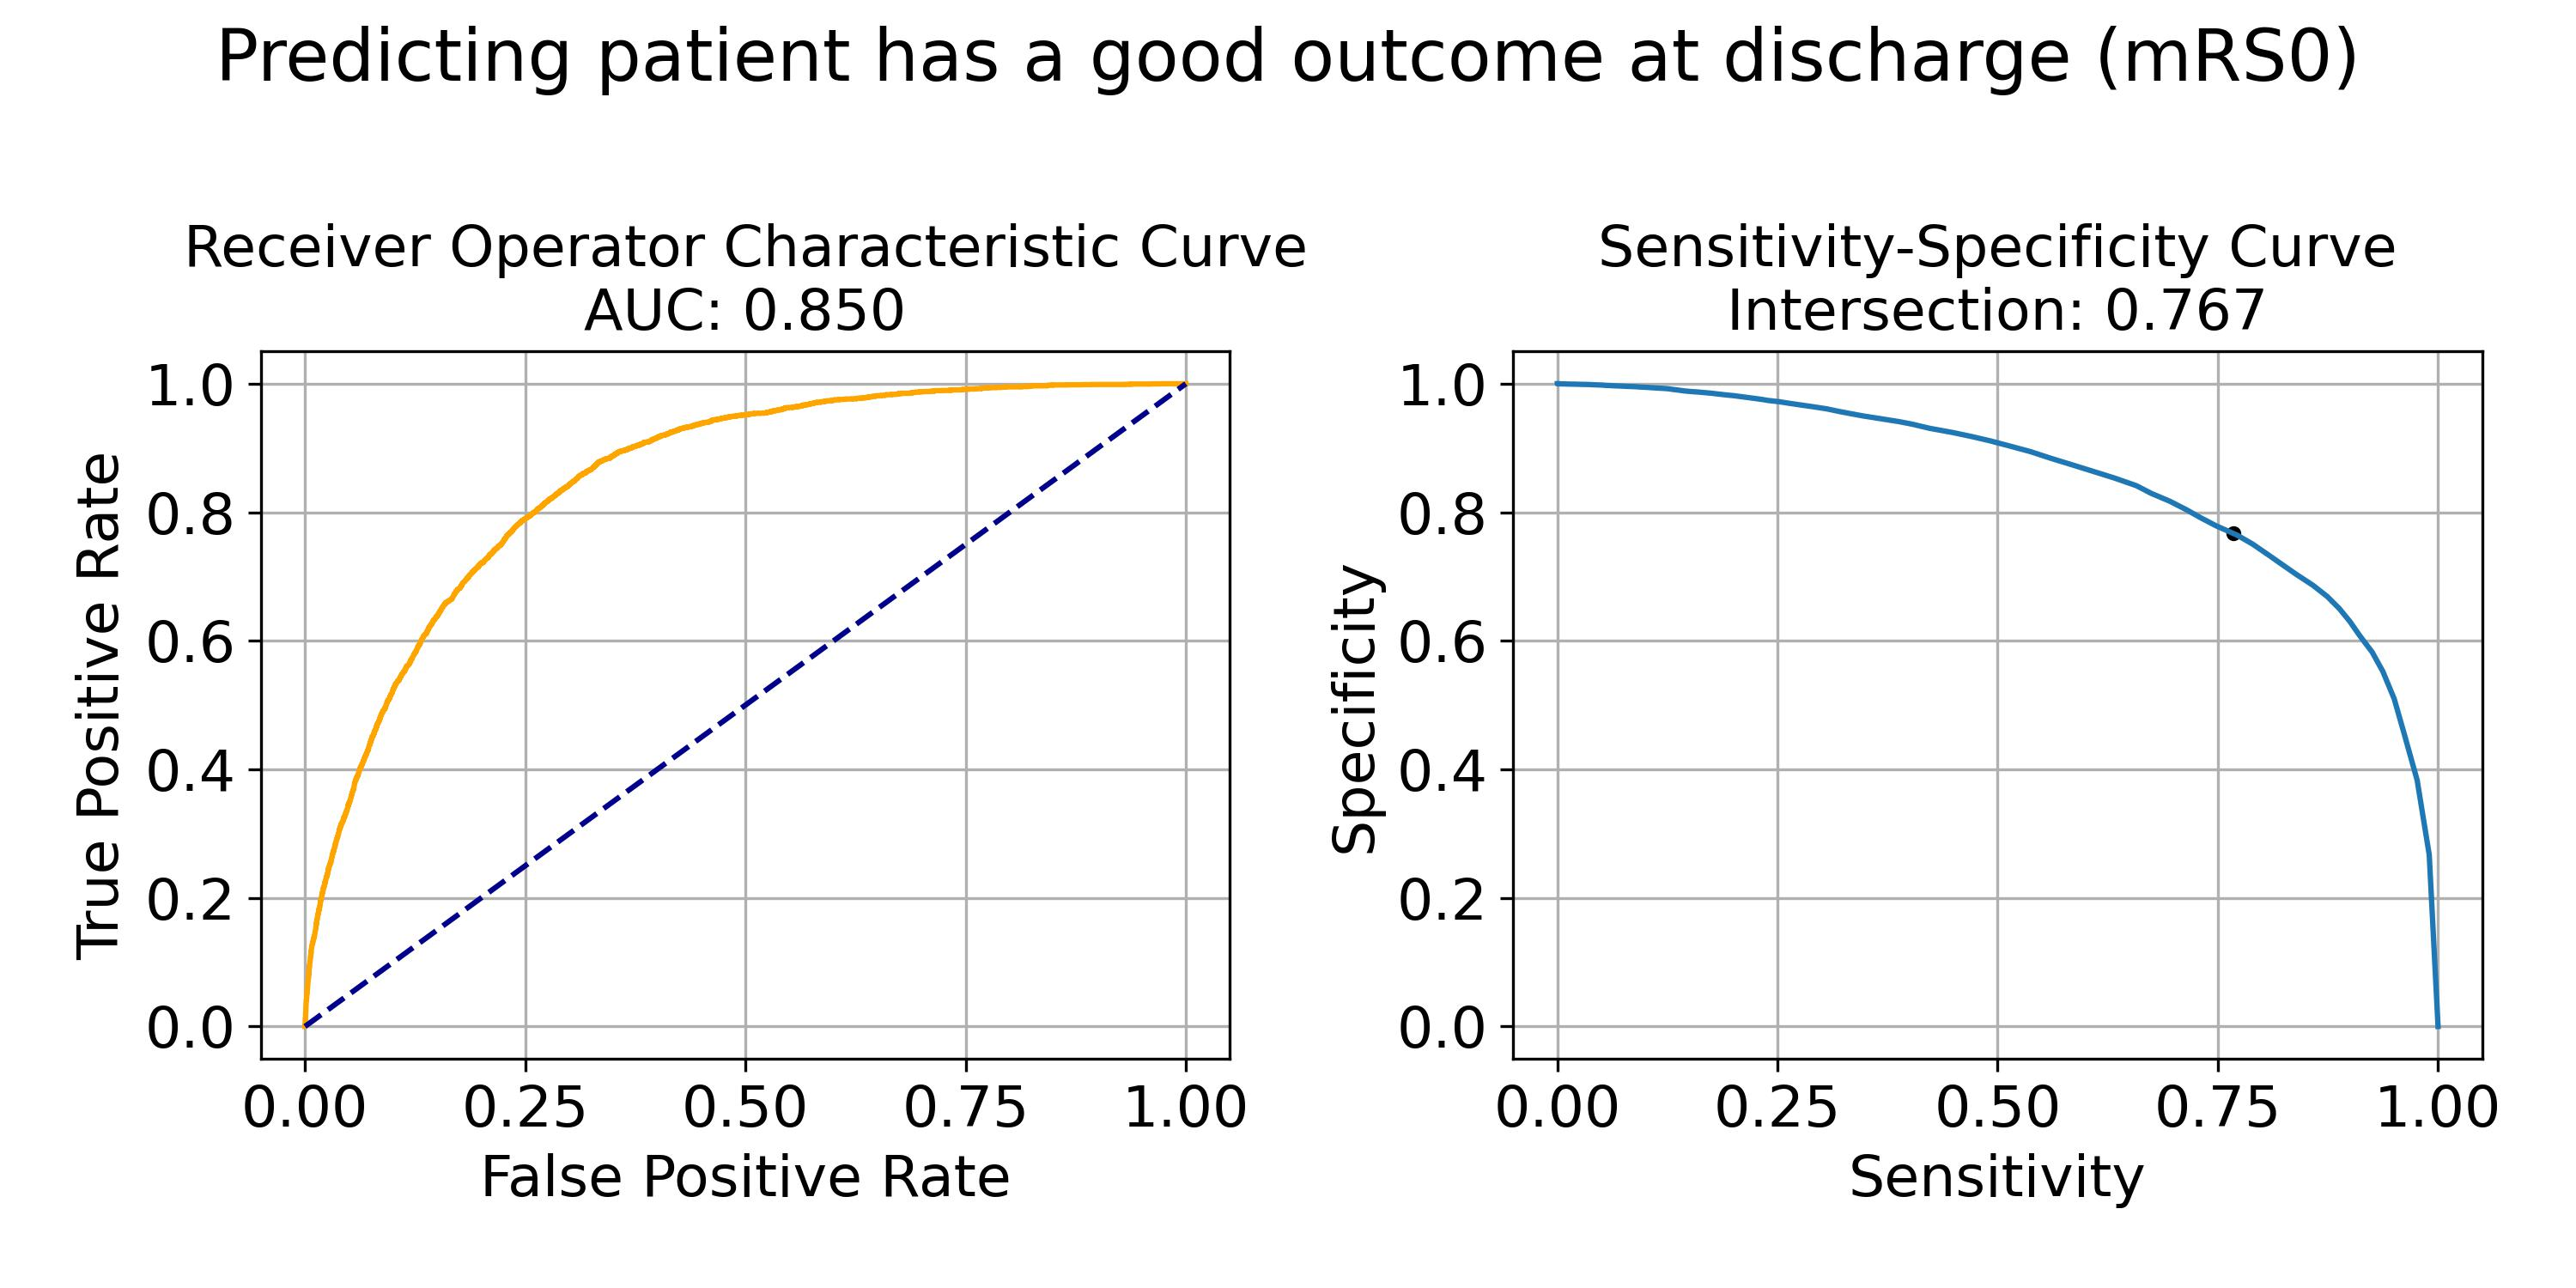
\includegraphics[width=0.5\linewidth]{./images/083_xgb_7_features_5fold_binary_roc_sens_spec_mrs0_kfold0_paper}}
\hfil
    \subfloat[]{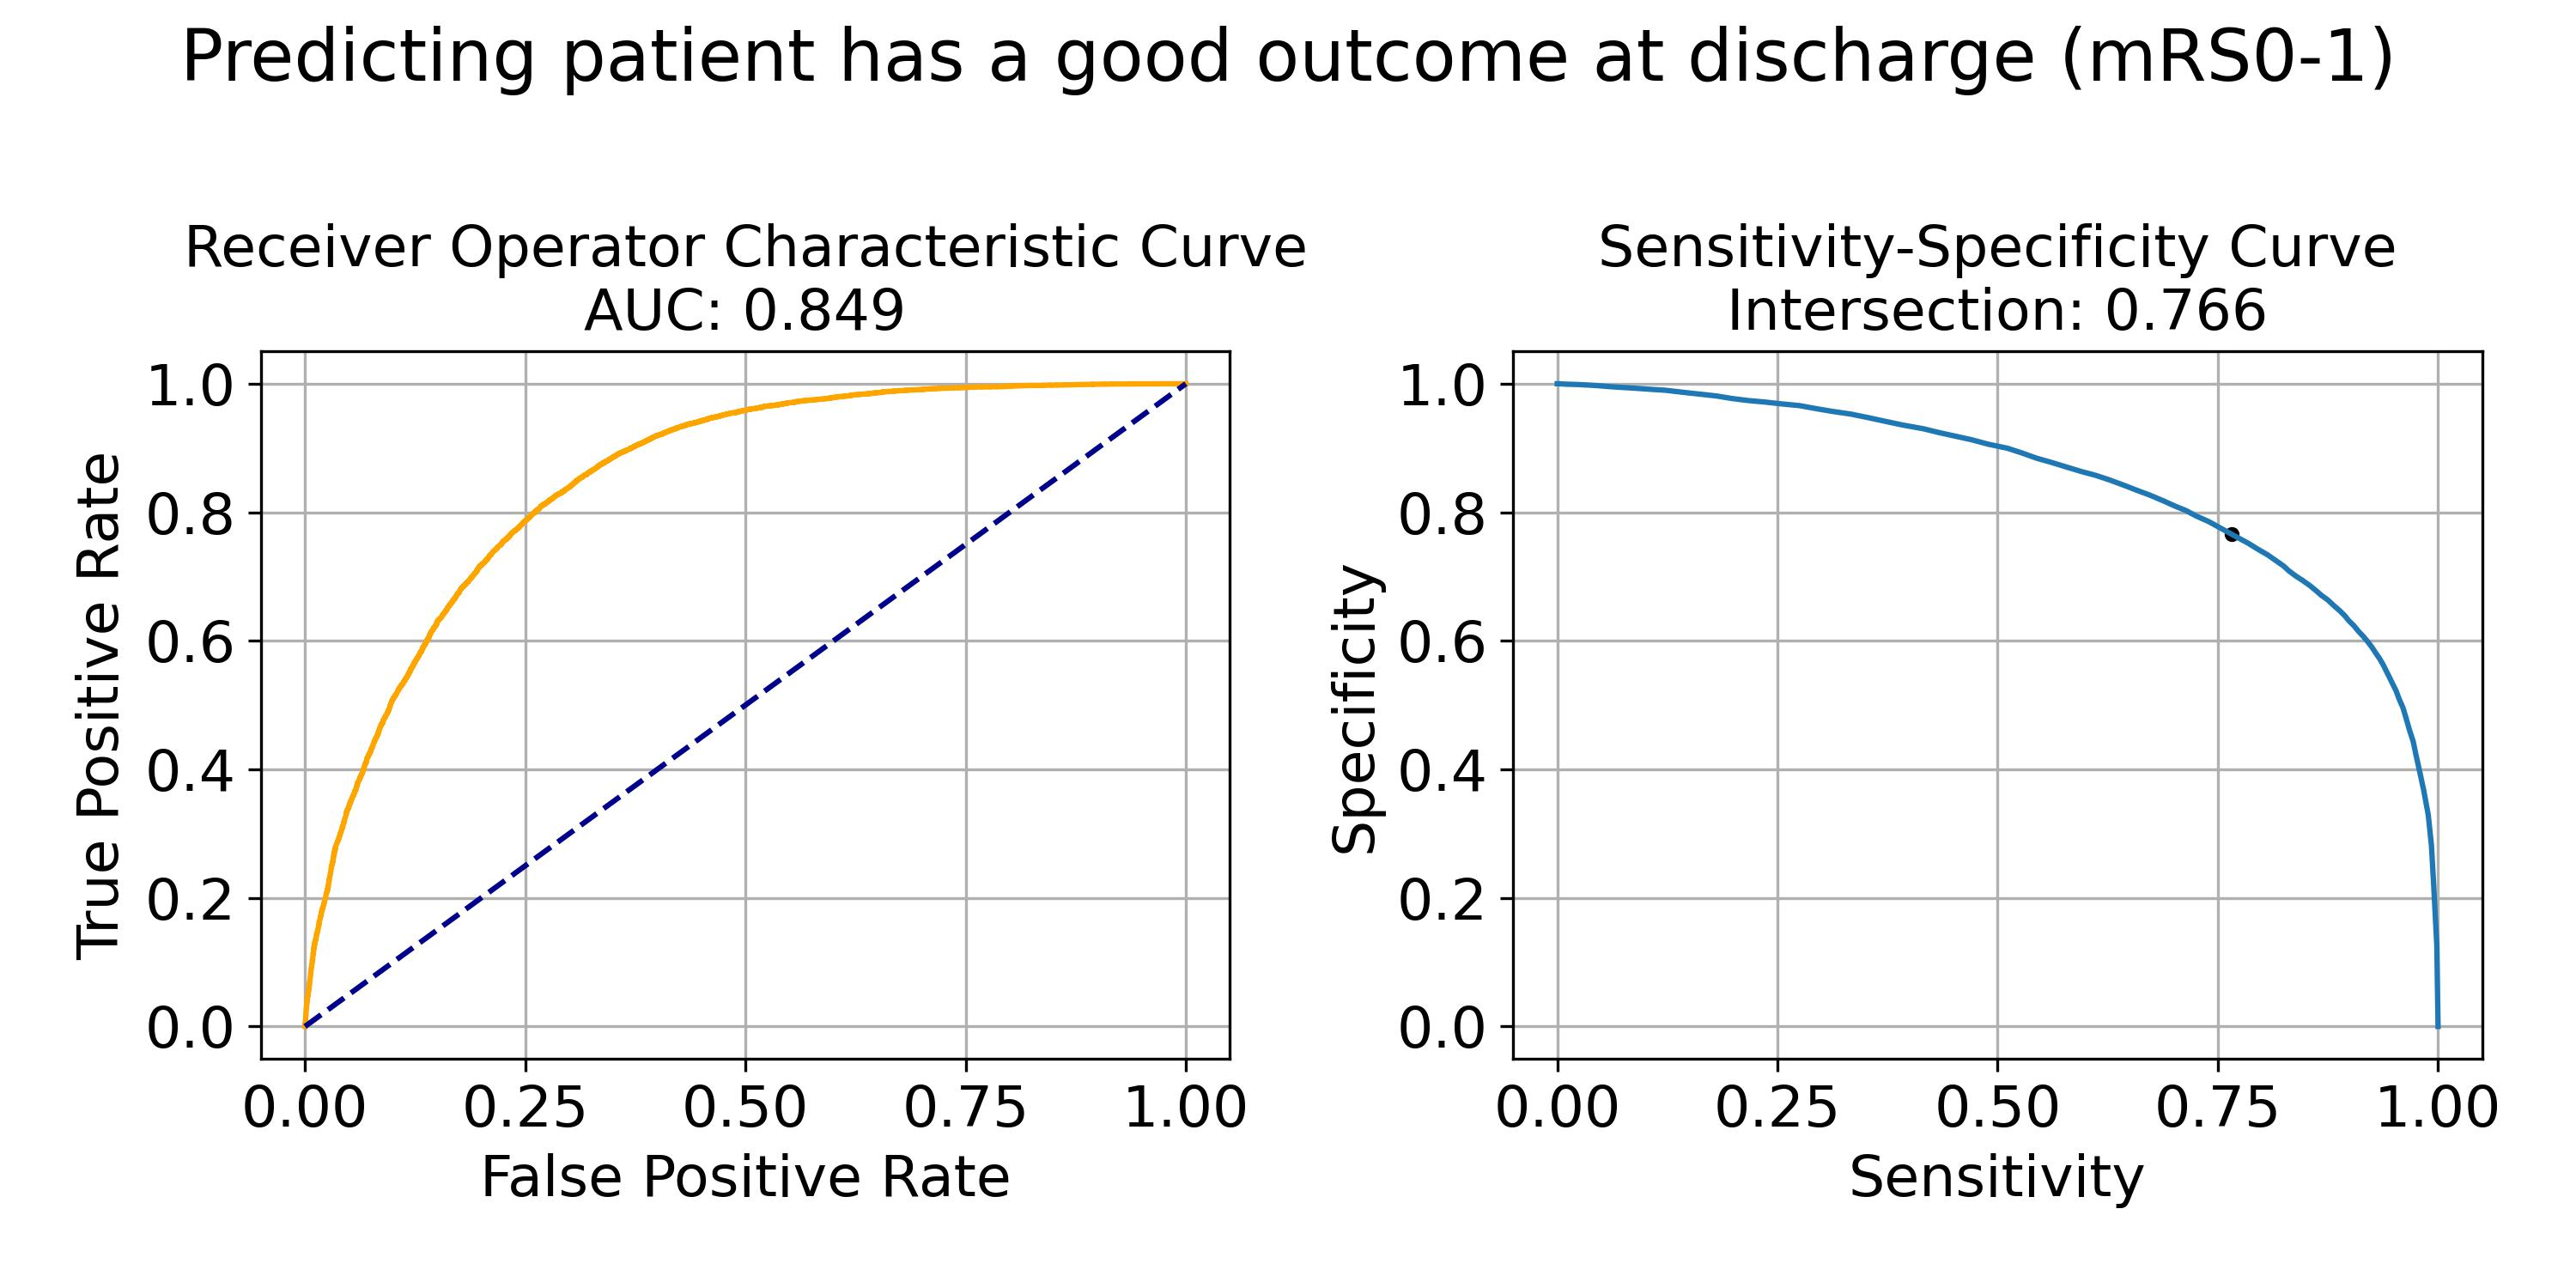
\includegraphics[width=0.5\linewidth]{./images/083_xgb_7_features_5fold_binary_roc_sens_spec_mrs1_kfold0_paper}}

    \subfloat[]{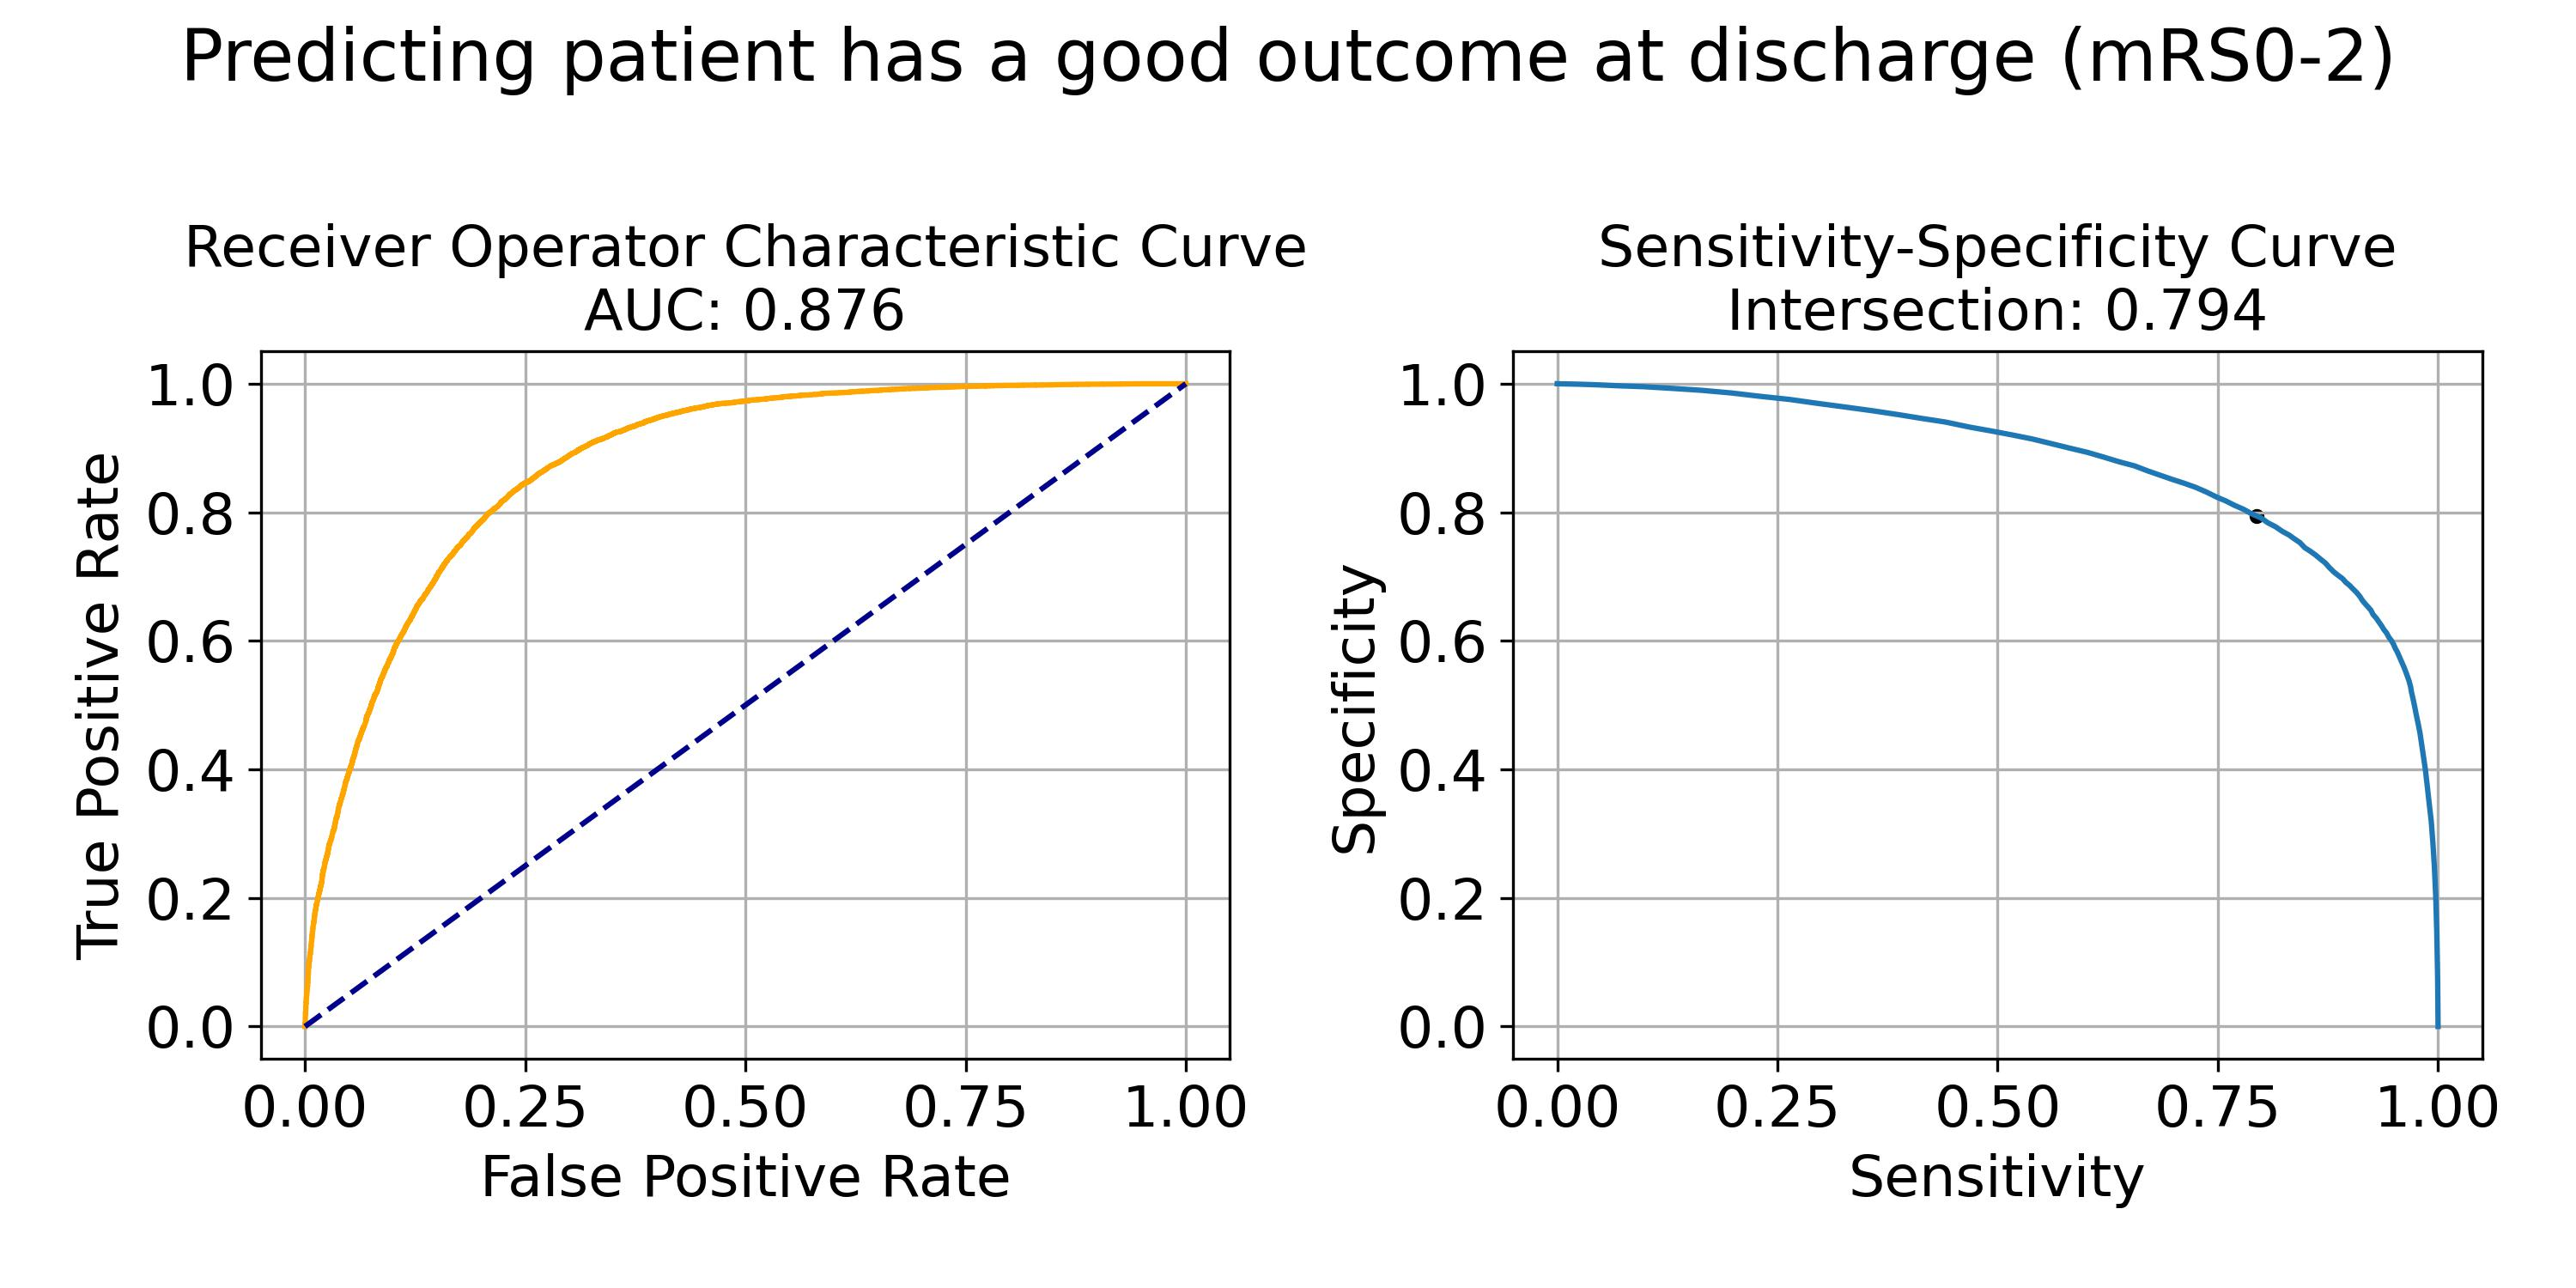
\includegraphics[width=0.5\linewidth]{./images/083_xgb_7_features_5fold_binary_roc_sens_spec_mrs2_kfold0_paper}}
\hfil
    \subfloat[]{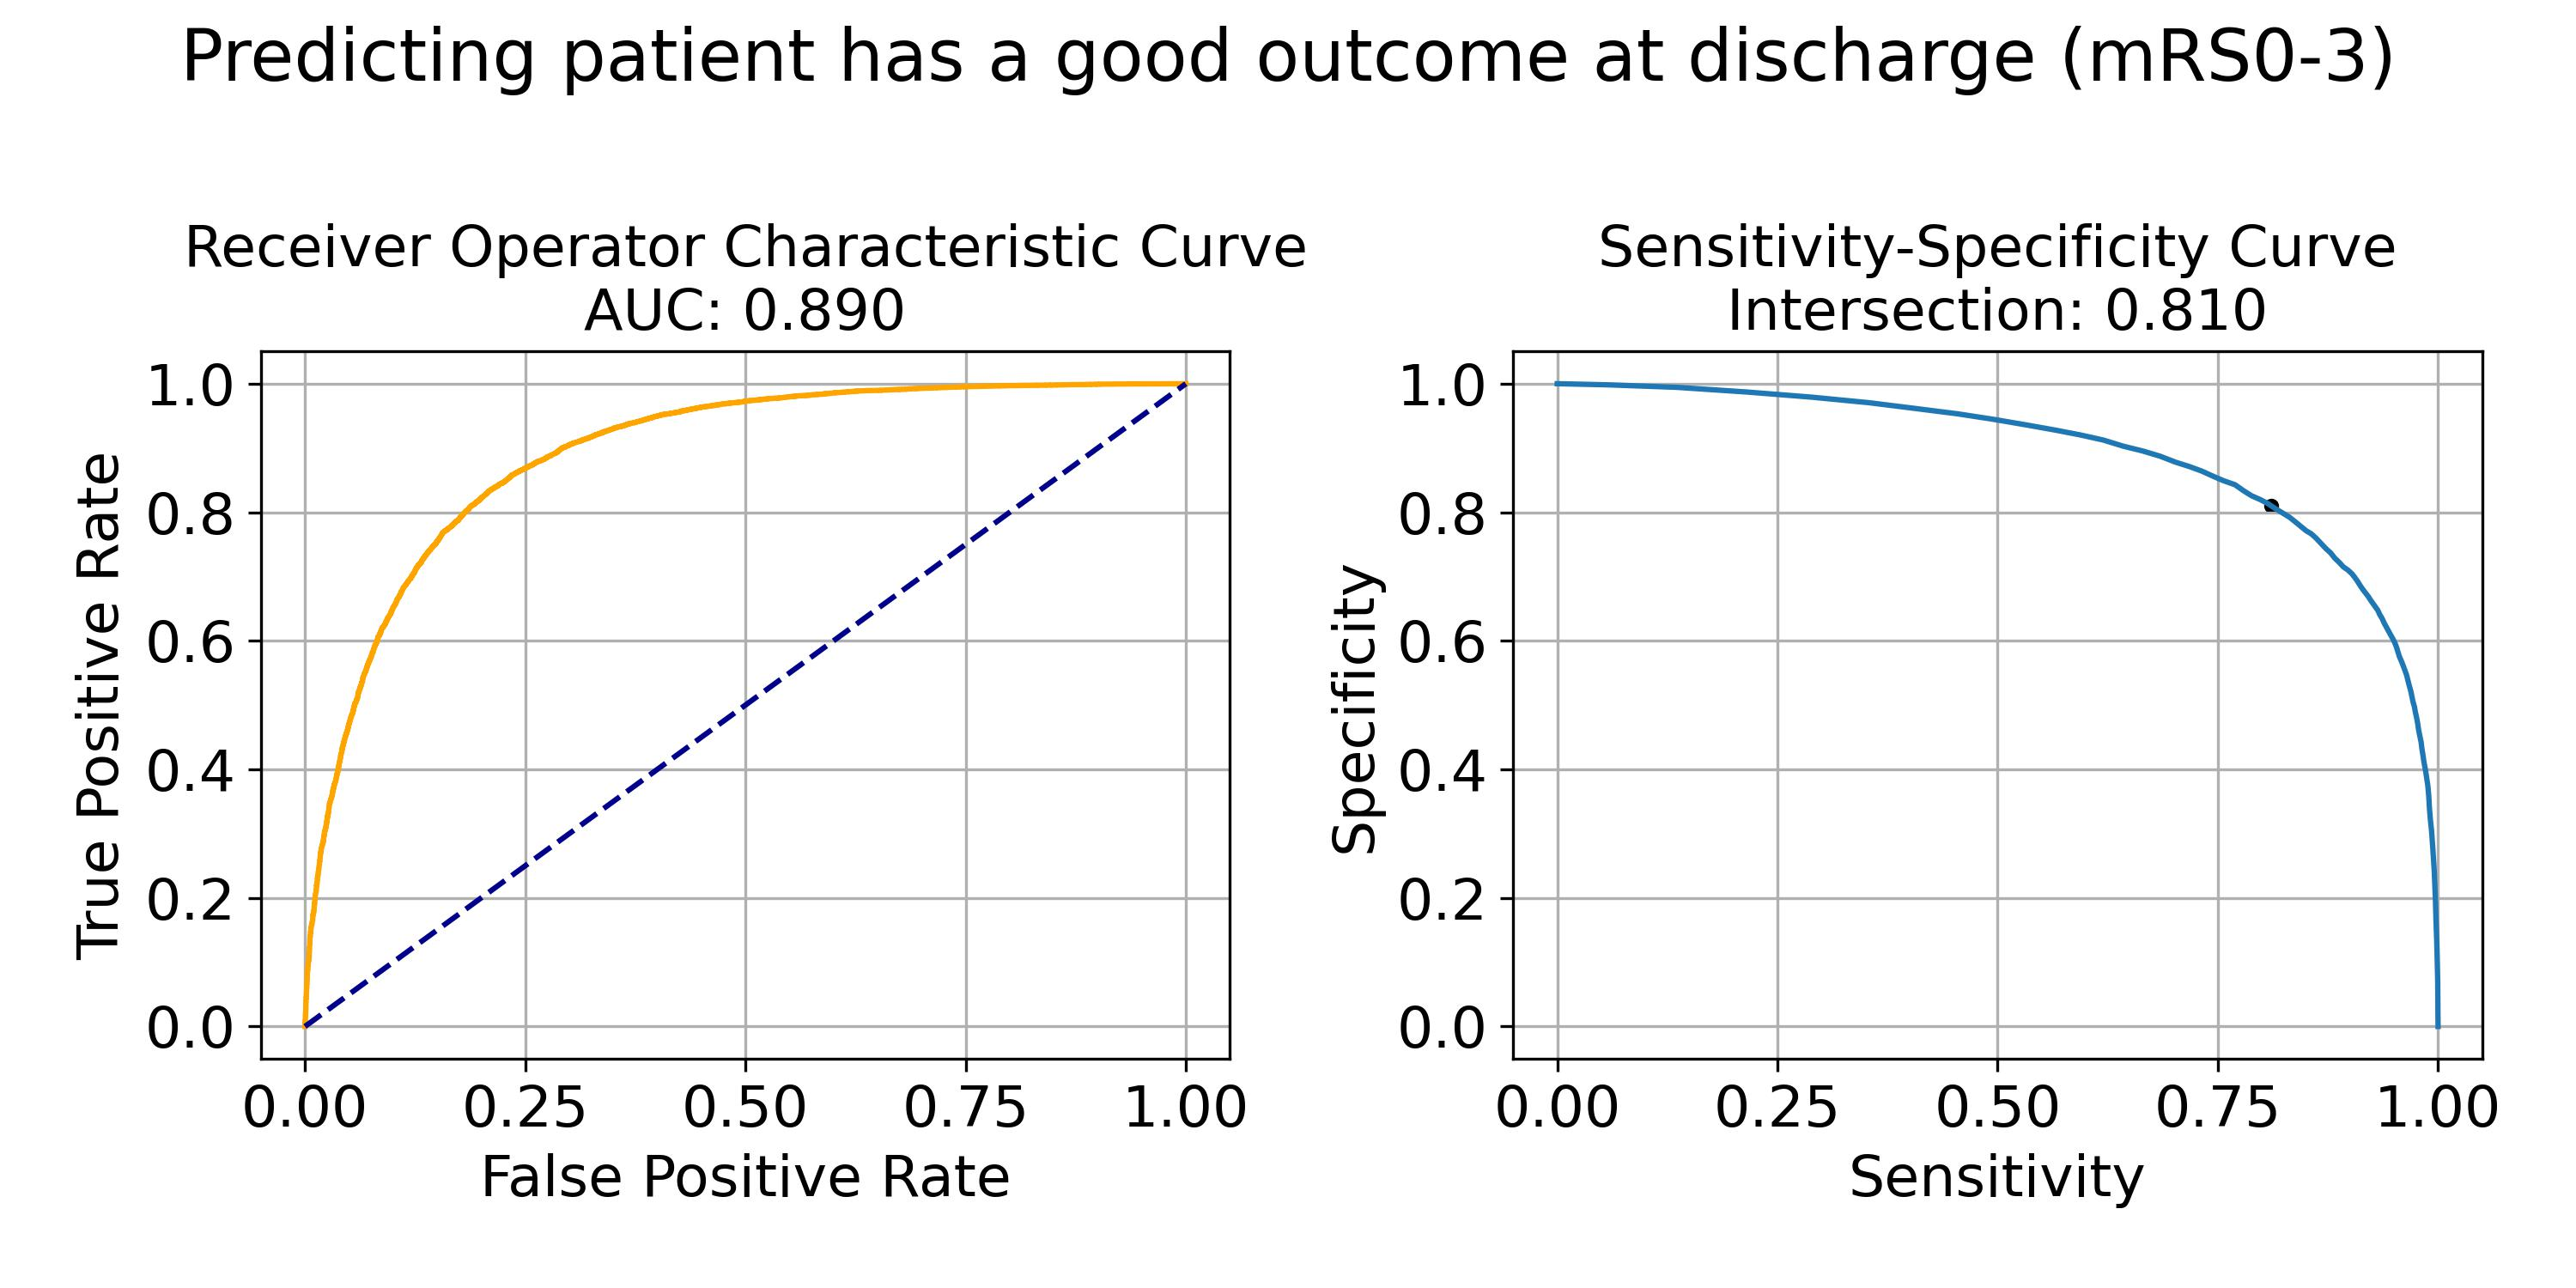
\includegraphics[width=0.5\linewidth]{./images/083_xgb_7_features_5fold_binary_roc_sens_spec_mrs3_kfold0_paper}}

    \subfloat[]{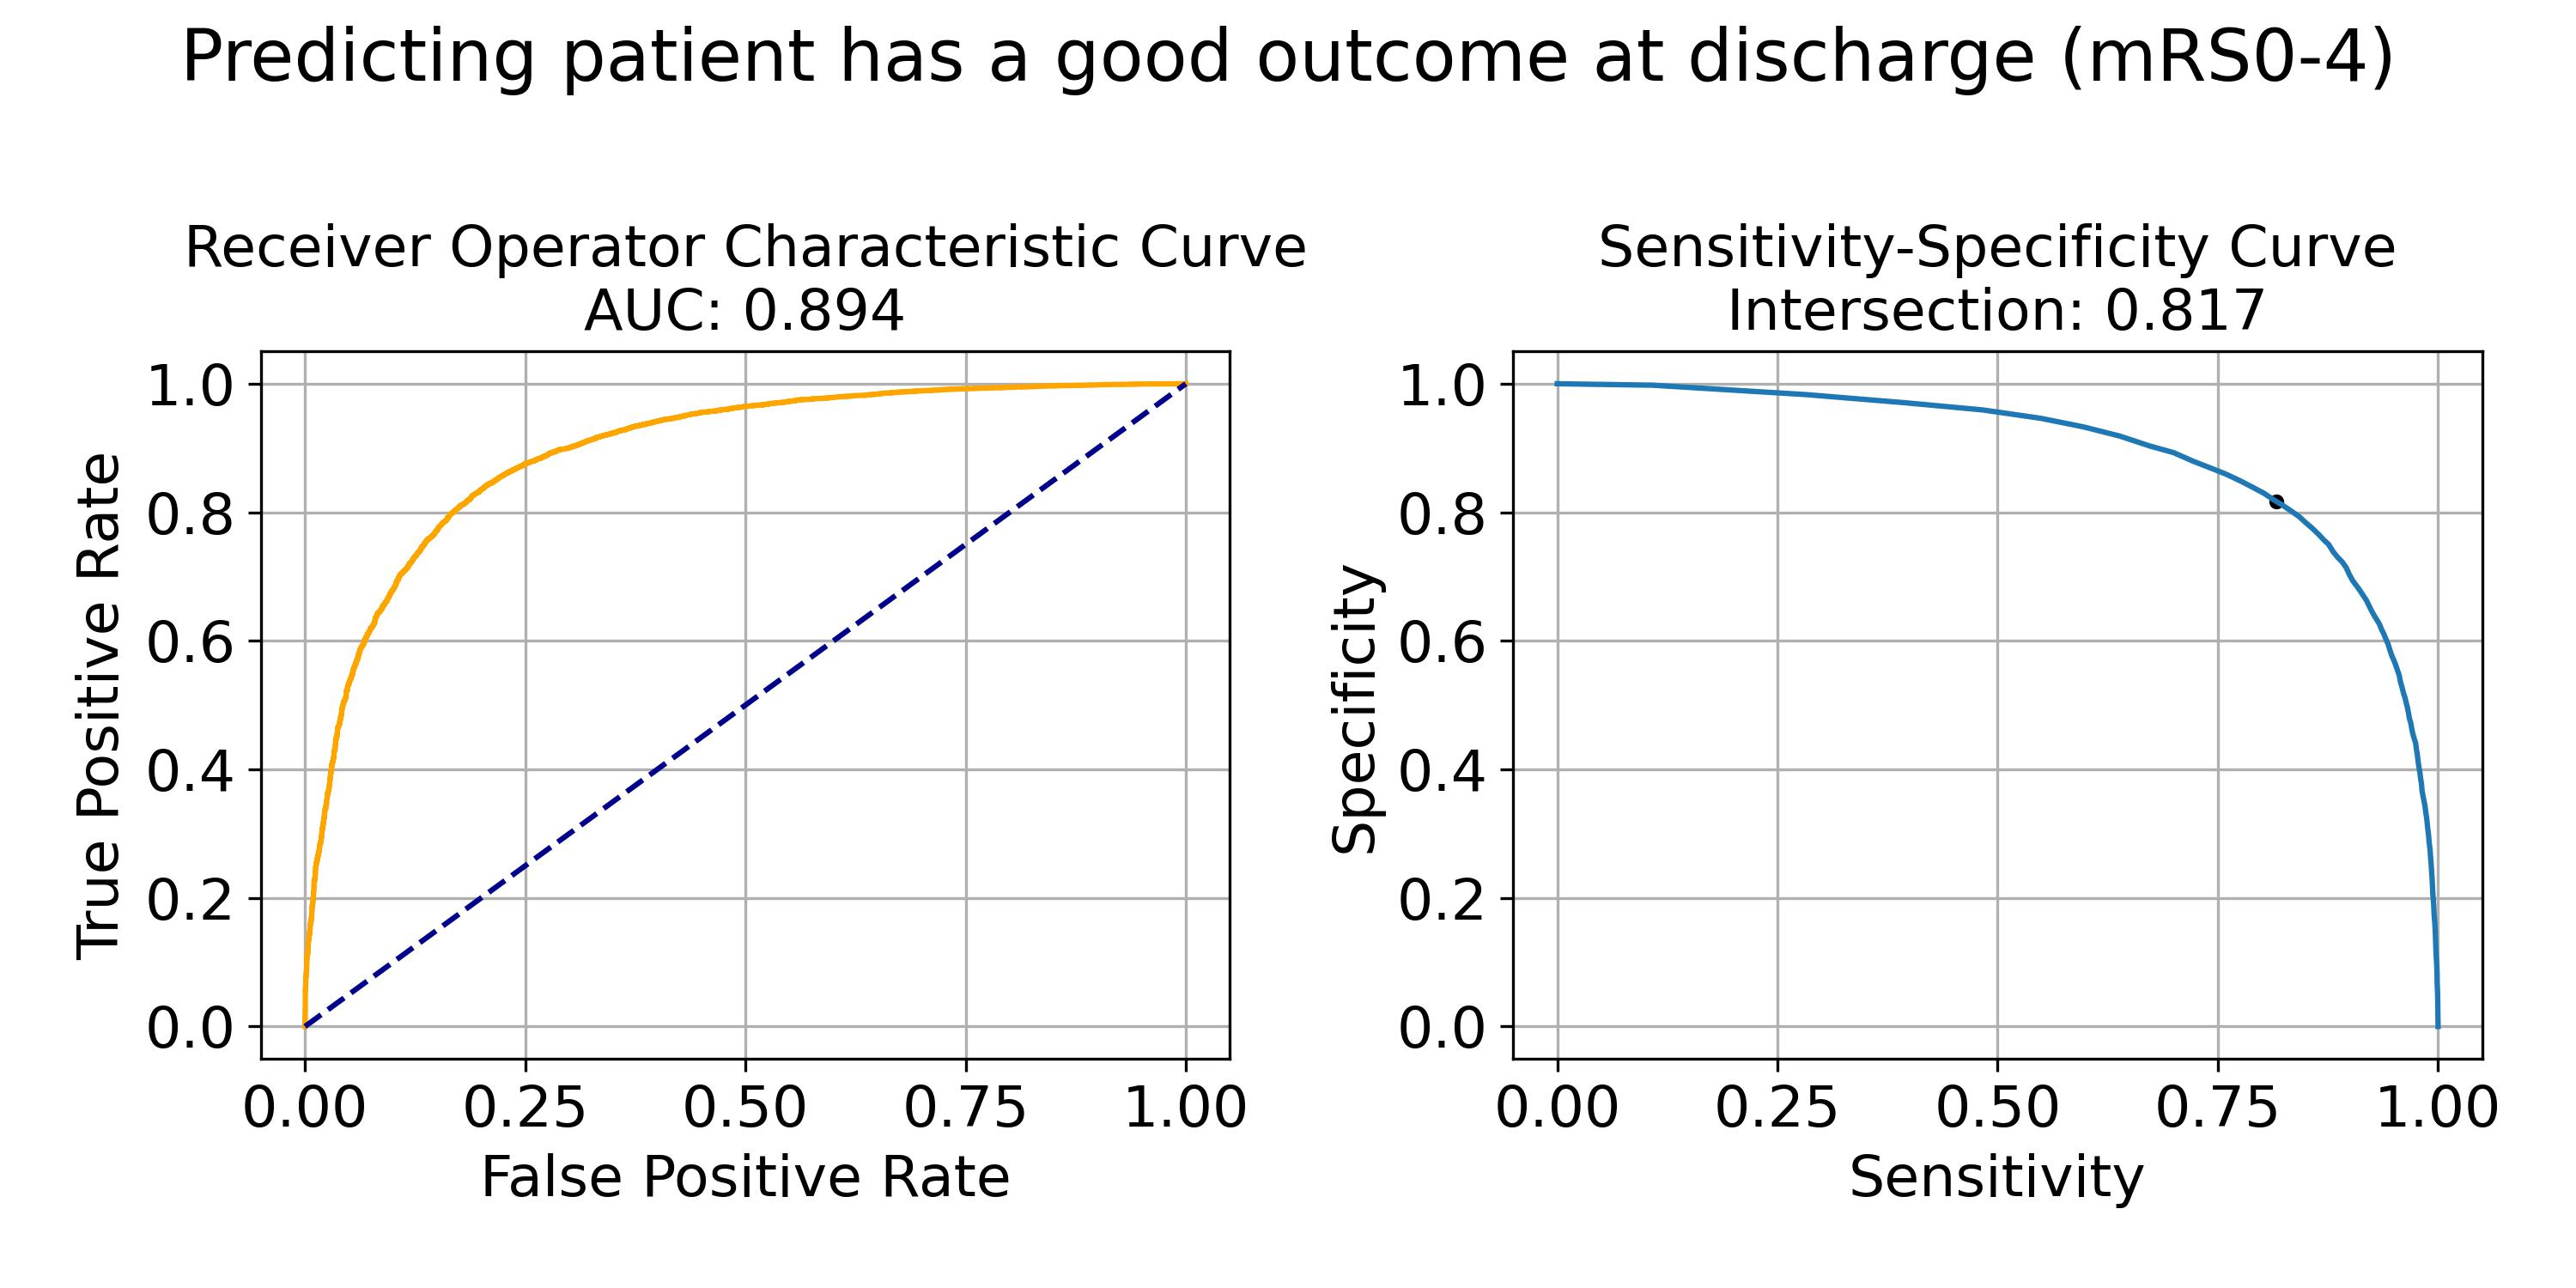
\includegraphics[width=0.5\linewidth]{./images/083_xgb_7_features_5fold_binary_roc_sens_spec_mrs4_kfold0_paper}}
\hfil
    \subfloat[]{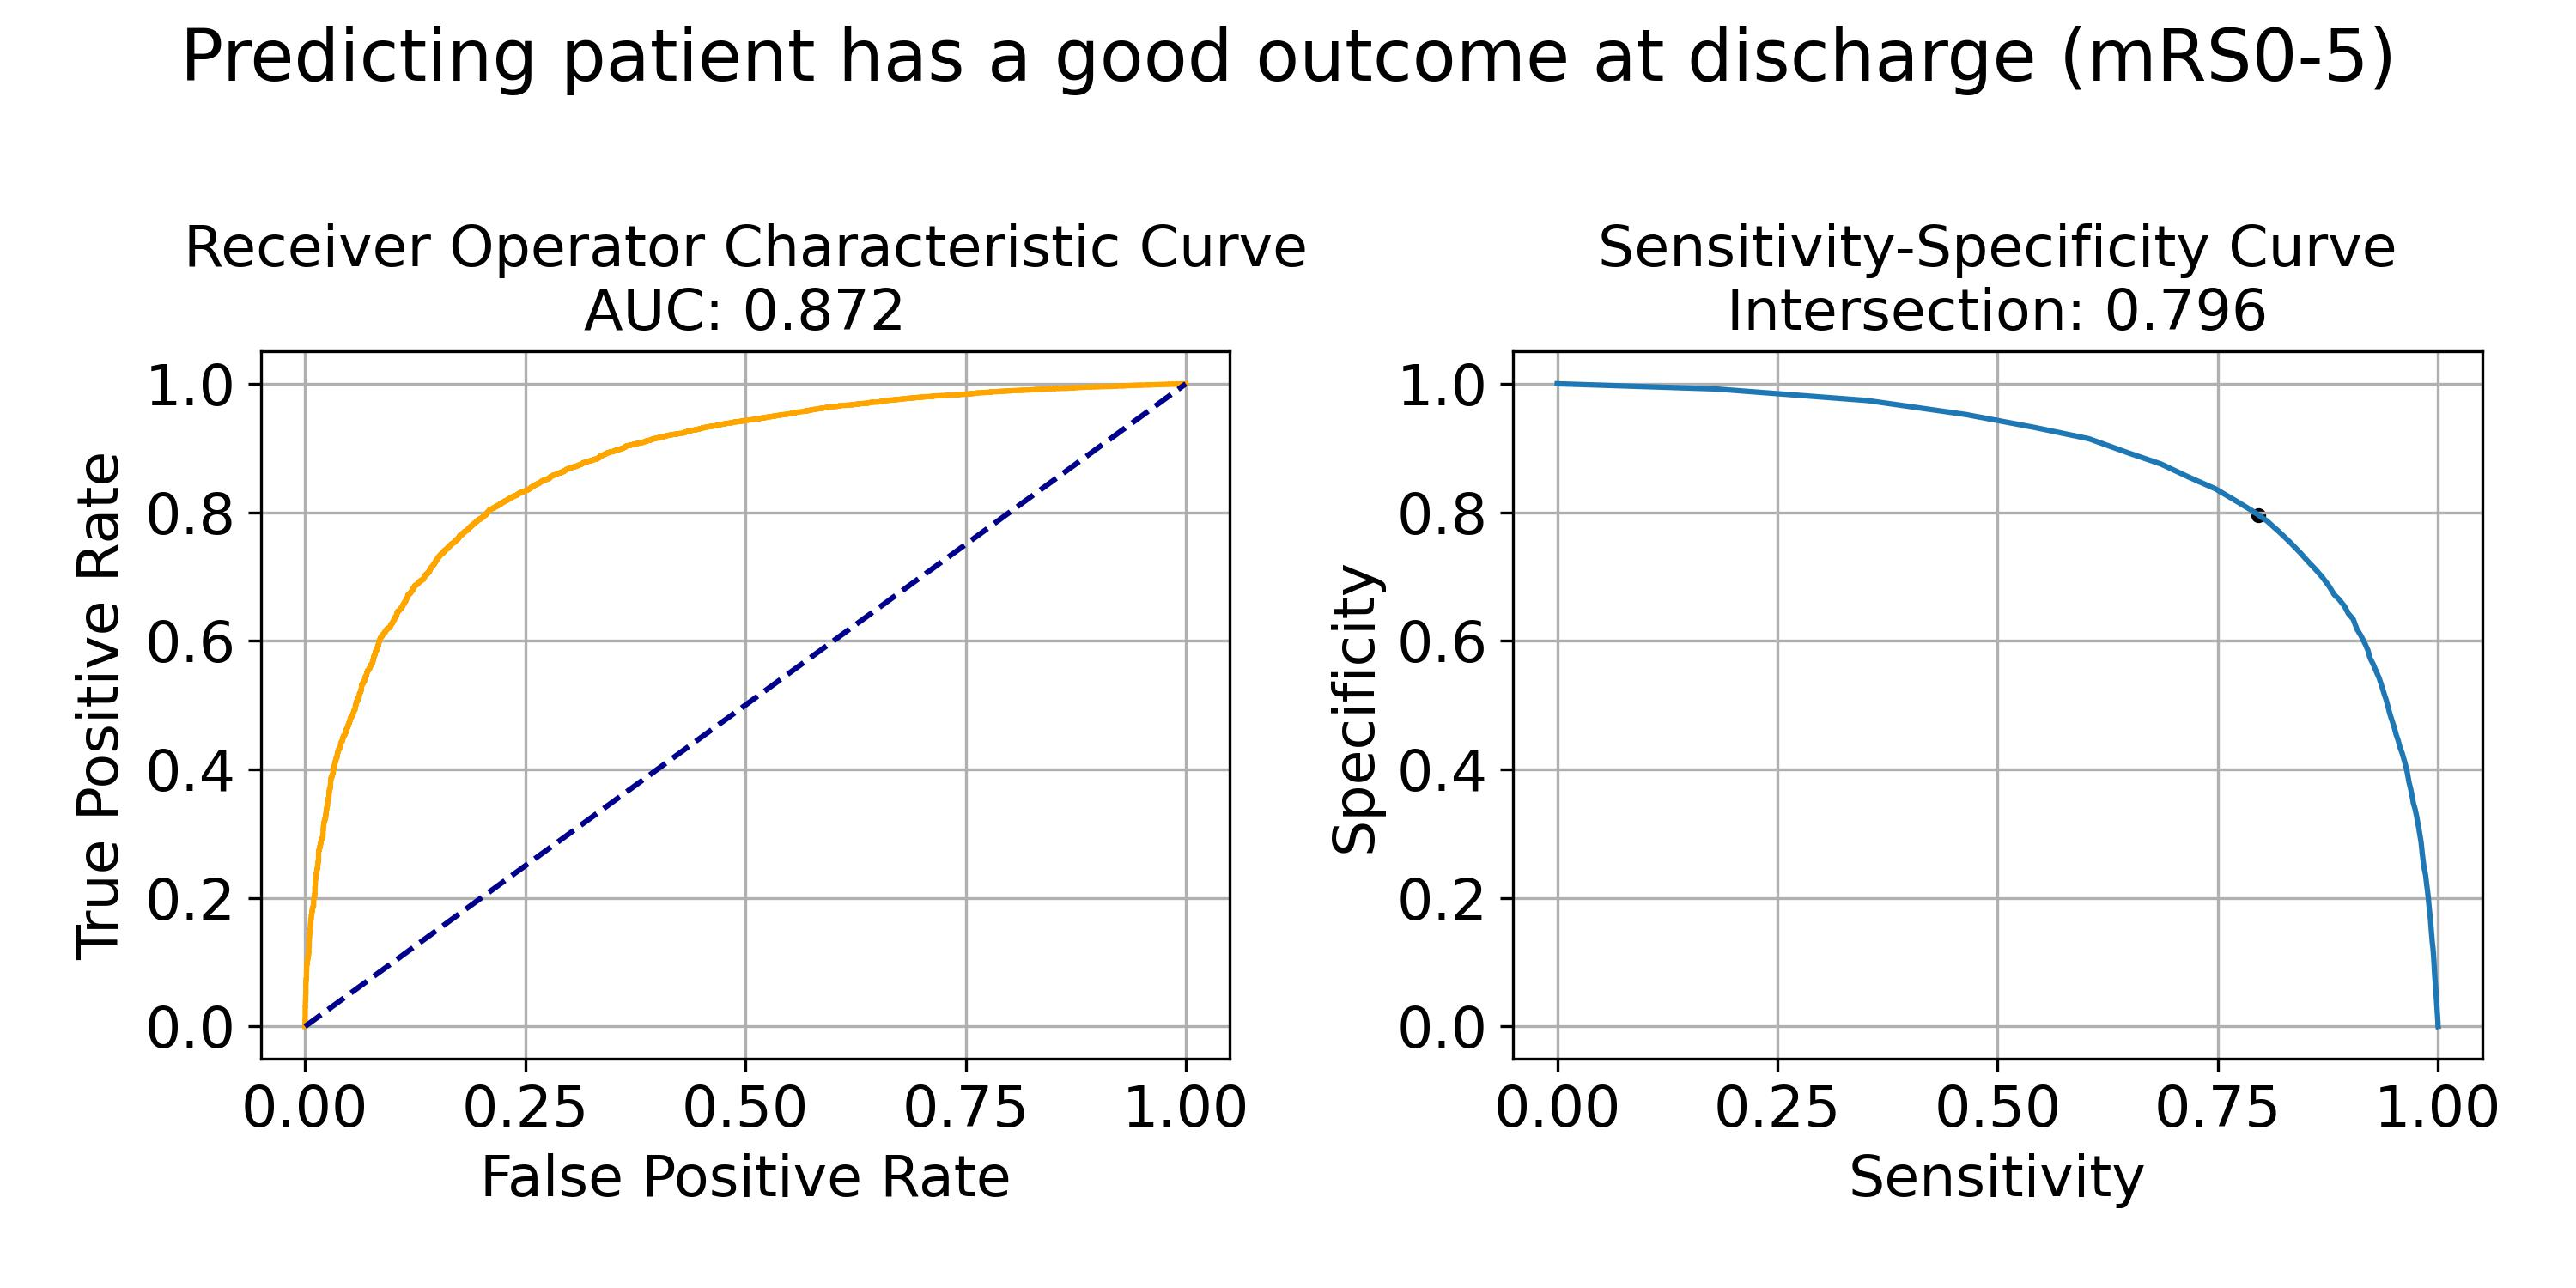
\includegraphics[width=0.5\linewidth]{./images/083_xgb_7_features_5fold_binary_roc_sens_spec_mrs5_kfold0_paper}}
    \label{fig:rocauc_ss}
  \caption{ROC AUC, and specificity and sensitivity plots for each of the mRS threshold levels to define a good outcome (for first kfold). Model has 7 inputs features.}

\end{figure}



\begin{figure}[!h]
    \centering
    \begin{subfigure}[b]{1\textwidth}
      \centering
      \includegraphics[width=1\textwidth]{./images/083_xgb_7_features_5fold_binary_shap_violin_0kfold}\\
      \caption{Kfold 1}
      \label{fig:results_waterfall}
    \end{subfigure}
\end{figure}
%    \hfill
%    \medskip
\begin{figure}[!h]\ContinuedFloat
    \begin{subfigure}[b]{1\textwidth}
      \centering    
      \includegraphics[width=1\textwidth]{./images/083_xgb_7_features_5fold_binary_shap_violin_1kfold}\\
      \caption{Kfold 2}
      \label{fig:results_waterfall}
    \end{subfigure}
\end{figure}
%    \hfill
%    \medskip
\begin{figure}[!h]\ContinuedFloat
    \begin{subfigure}[b]{1\textwidth}
      \centering
      \includegraphics[width=1\textwidth]{./images/083_xgb_7_features_5fold_binary_shap_violin_2kfold}\\
      \caption{Kfold 3}
      \label{fig:results_waterfall}
    \end{subfigure}
\end{figure}
%    \hfill
%    \medskip
\begin{figure}[!h]\ContinuedFloat
    \begin{subfigure}[b]{1\textwidth}
      \centering
      \includegraphics[width=1\textwidth]{./images/083_xgb_7_features_5fold_binary_shap_violin_3kfold}\\
      \caption{Kfold 4}
      \label{fig:results_waterfall}
    \end{subfigure}
\end{figure}
%    \hfill
%    \medskip
\begin{figure}[!h]\ContinuedFloat
    \begin{subfigure}[b]{1\textwidth}
      \centering
      \includegraphics[width=1\textwidth]{./images/083_xgb_7_features_5fold_binary_shap_violin_4kfold}\\
      \caption{Kfold 5}
      \label{fig:results_waterfall}
    \end{subfigure}
  \caption{Violin plots show SHAP values vs feature values for each feature, a sub figure for each kfold}
\end{figure}



%%%%%%%%%%%% 3.6.3  %%%%%%%%%%%%%%%%%
\subsubsection{The direct contribution of thrombolysis use to the shift in probability of a good outcome - for all definitions of a good outcome (3.6.3 extension)}

Using the counterfactual results for all of the patients in the first k-fold test set that received thrombolysis, figure \ref{fig:shap_shift_lvo_nlvo} shows a linear regression fitted to the shift in the contribution from receiving thrombolysis towards having a good outcome at discharge (mRS0-1) with respect to the onset to thrombolysis time. 

Figures \ref{fig:stats_table_common_odds_ratio} and \ref{fig:stats_table_mrs1} show that the linear regression coefficients are statistically significant. Taking mRS 0-1 as a good outcome, we found that the effect of thrombolysis had declined to zero at 328 minutes, and the effect from thrombolysis was improving odds of a good outcome by 0.90 if it were, theoretically, given at the time of stroke onset. Figure \ref{fig:shap_shift_lvo} shows results for the patient cohort with a severe stroke severity (NIHSS 11+). Figure \ref{fig:shap_shift_nlvo} shows results for the patient cohort with a mild-moderate stroke severity (NIHSS 0-10). Linear regression coefficients in both groups were statistically significant (figures \ref{fig:stats_table_common_odds_ratio} and \ref{fig:stats_table_mrs1}). We observed that the maximum theoretical effect of thrombolysis (if given at time of stroke onset) was greater for the severe stroke group (1.048 log odds for mRS0-1) than the mild-moderate stroke group (0.771 log odds for mRS0-1). However the effect of thrombolysis declined a little faster in the severe stroke group (reaching no effect at 314 minutes, compared to 351 minutes for mild-moderate stroke patients).

\begin{figure}[!ht]
    \centering
    \begin{subfigure}[b]{.7\textwidth}
      \centering
      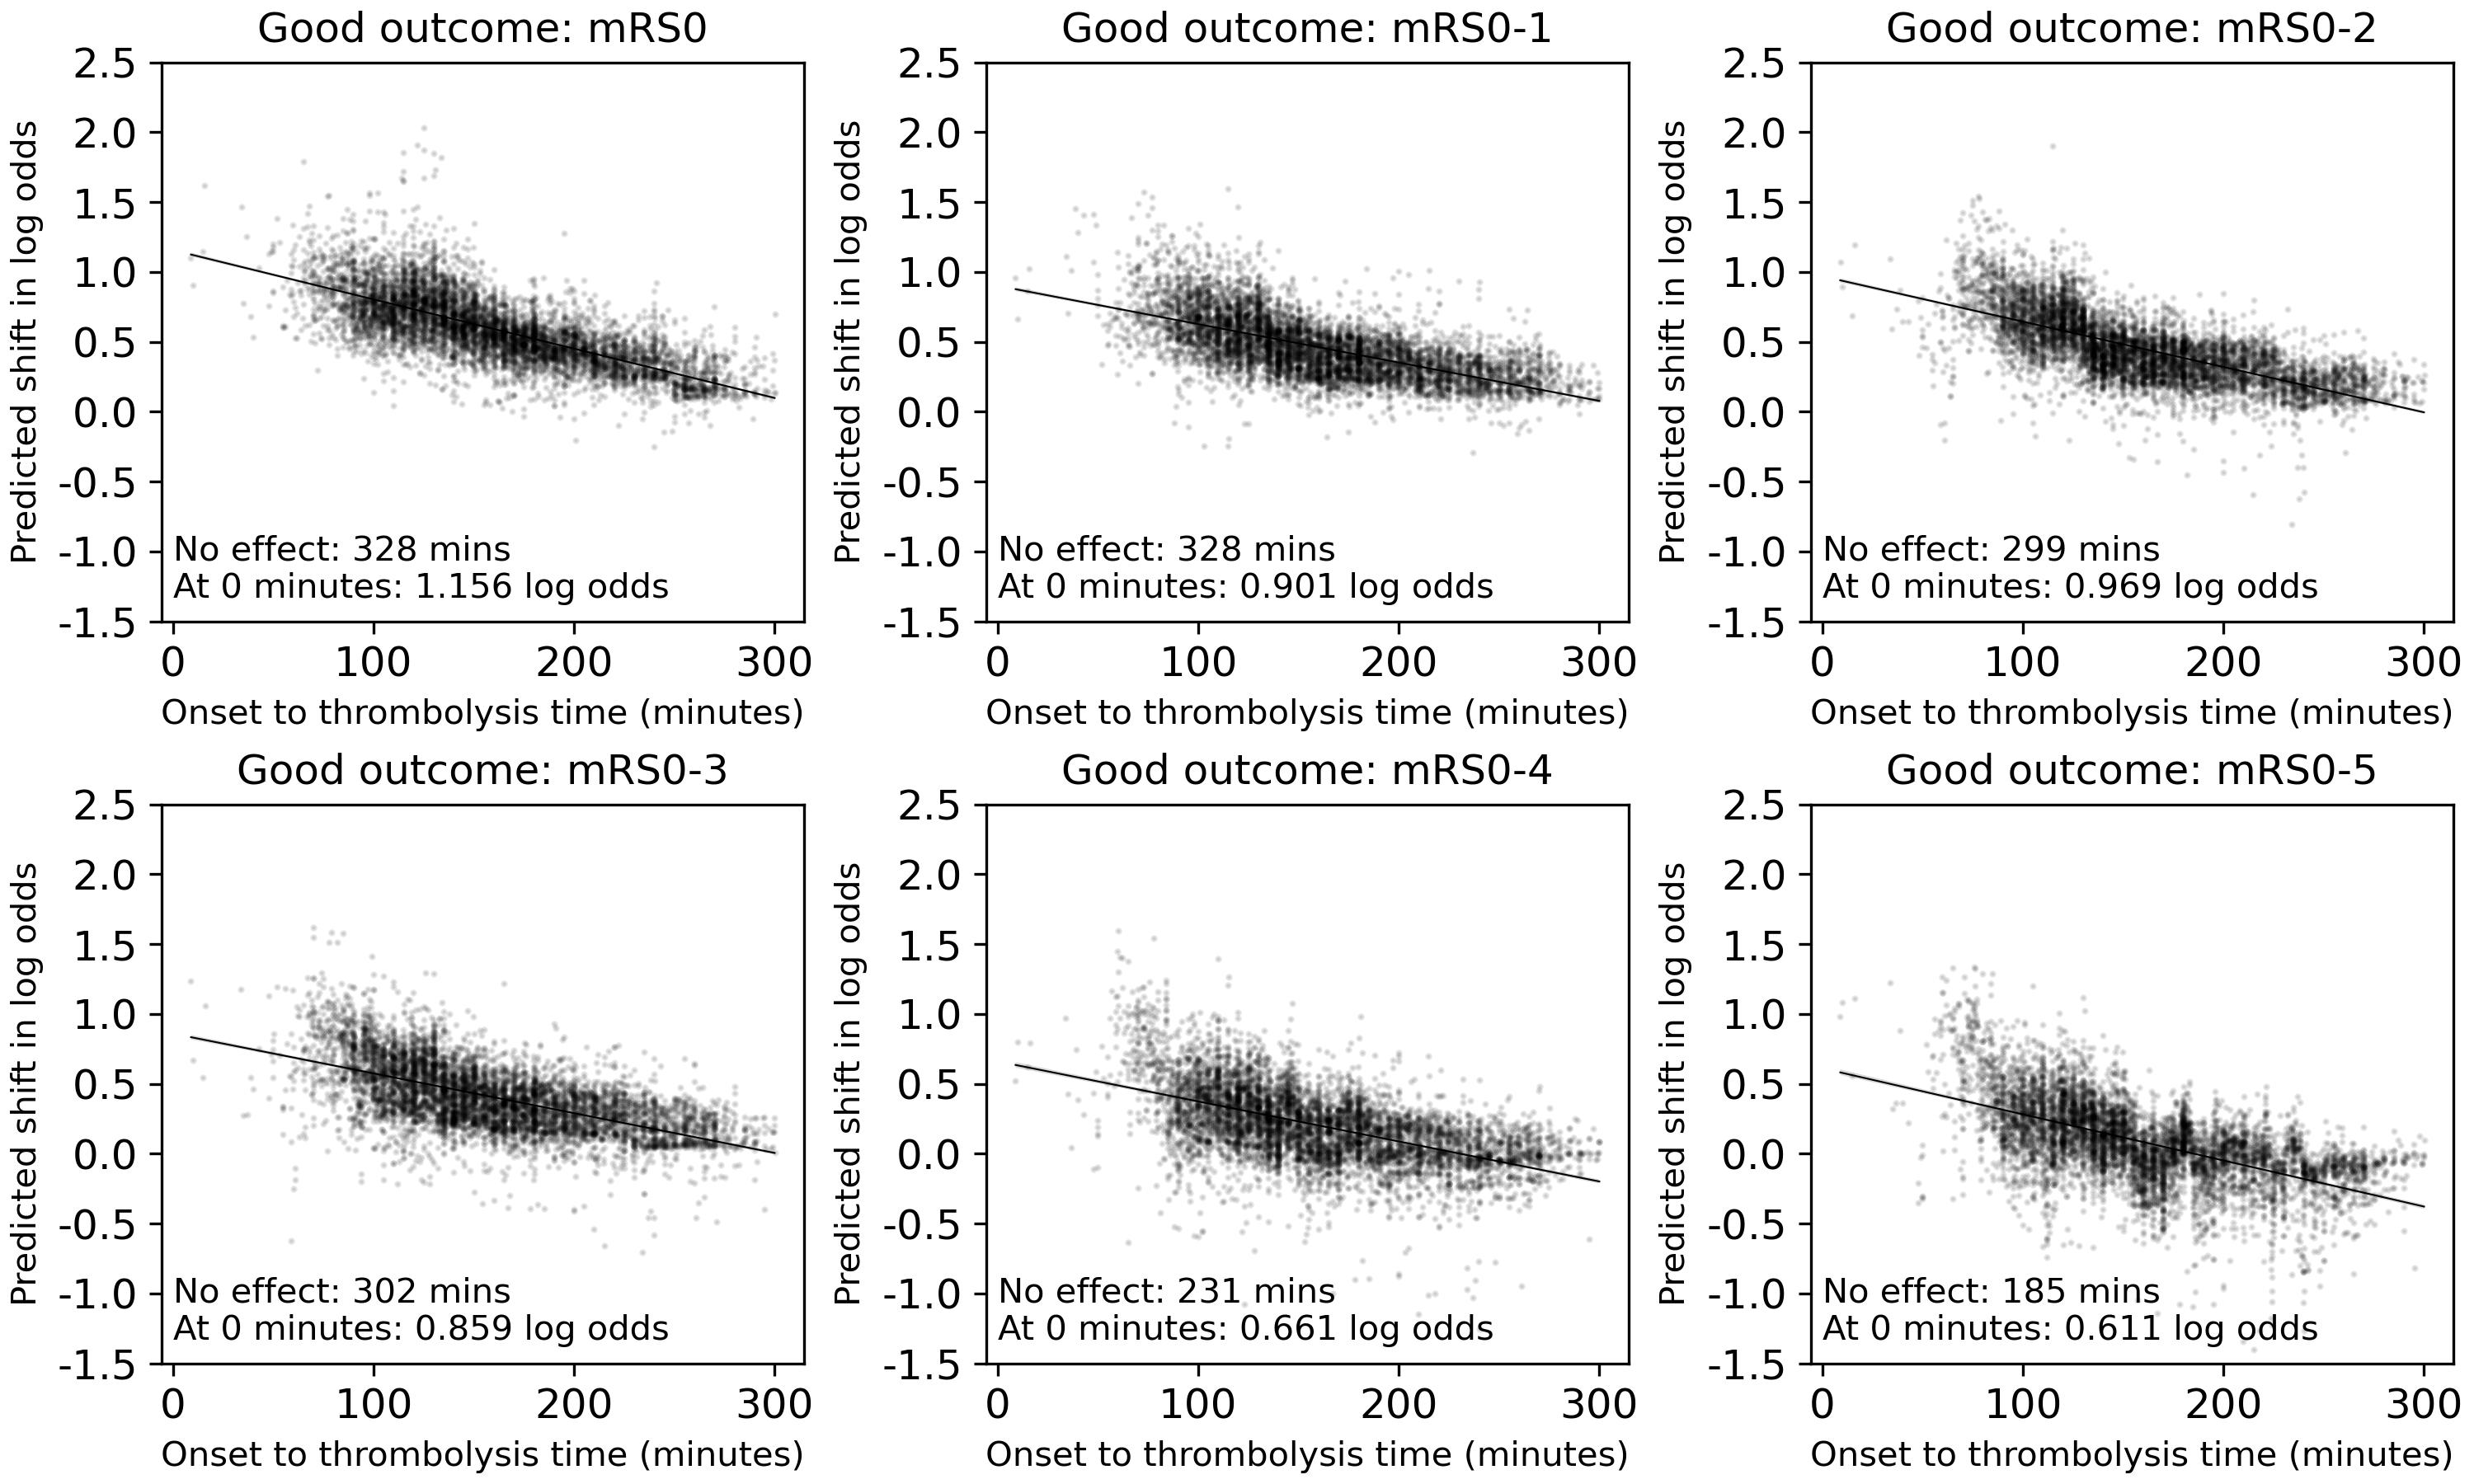
\includegraphics[width=1\textwidth]{./images/103_xgb_7_features_1fold_binary_improvement_logodds_bymRSthreshold_sns_6_subplots_nLVO_LVO_ivt_shap_paper}\\
      \caption{Patients in the test set that received thrombolysis}
      \label{fig:shap_shift_lvo_nlvo}
    \end{subfigure}
    \hfill
    \begin{subfigure}[b]{.7\textwidth}
      \centering    
      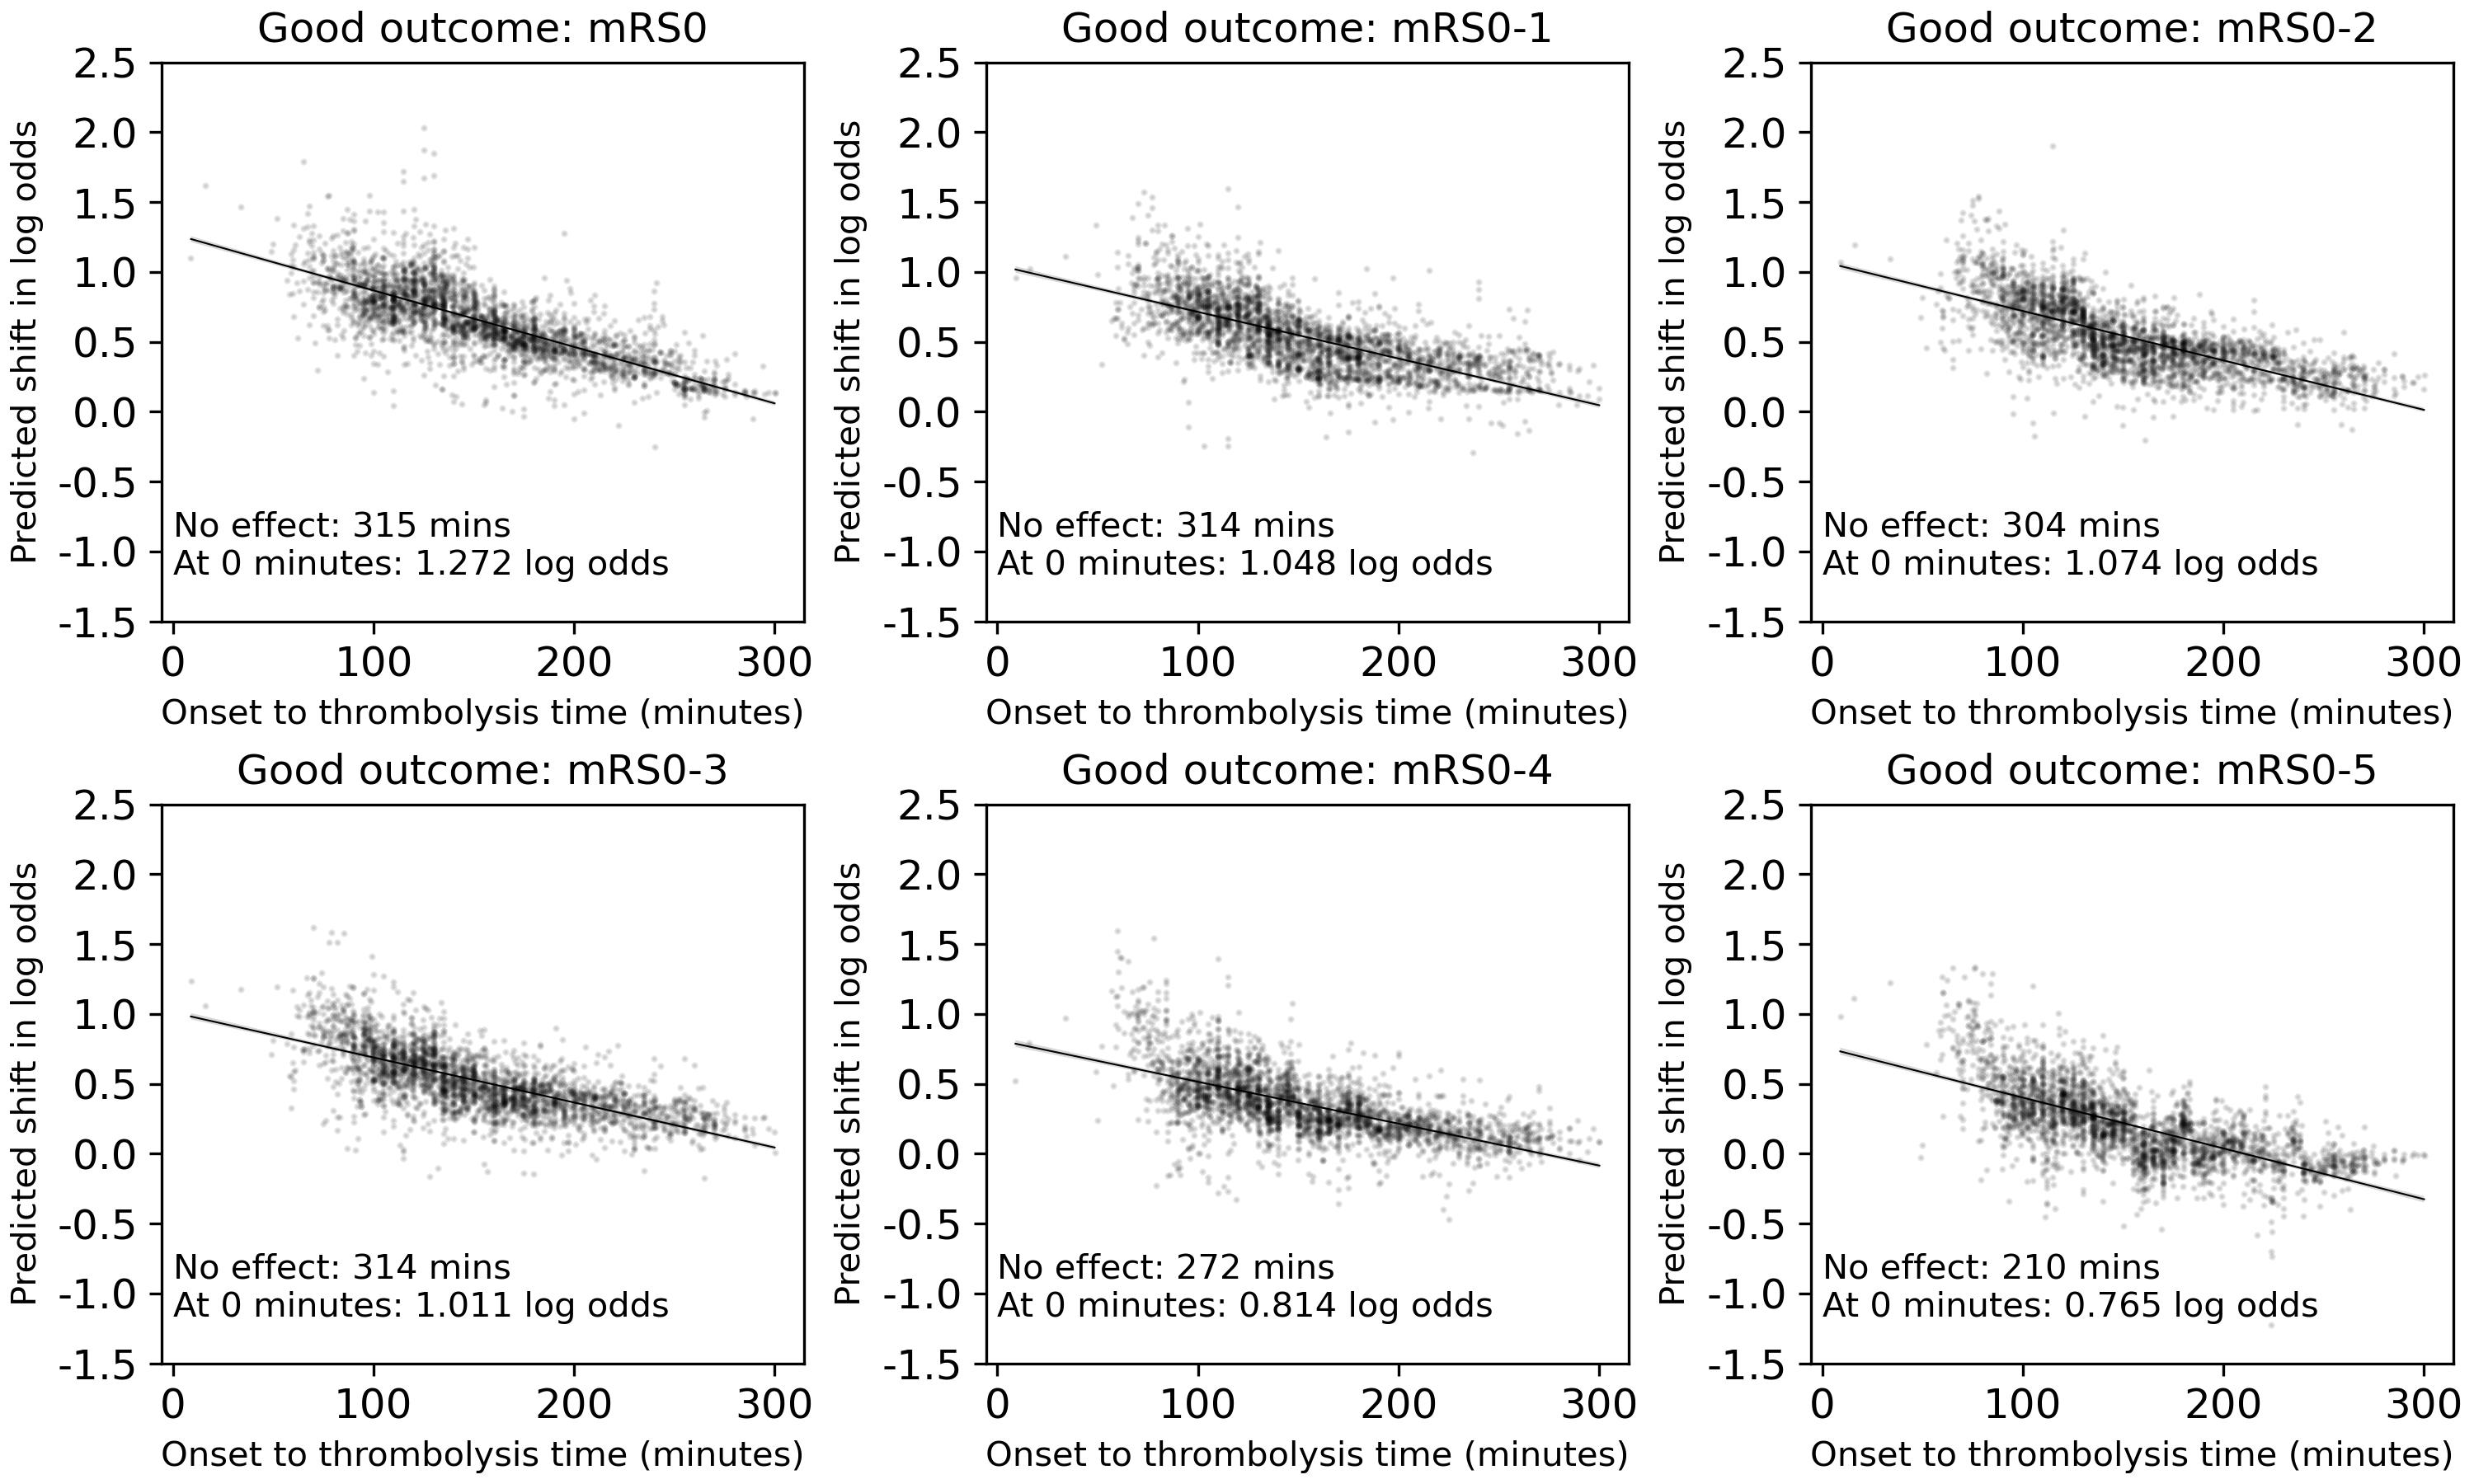
\includegraphics[width=1\textwidth]{./images/103_xgb_7_features_1fold_binary_improvement_logodds_bymRSthreshold_sns_6_subplots_LVO_ivt_shap_paper}\\
      \caption{Patients in the test set that received thrombolysis with severe stroke (NIHSS 11+)}
      \label{fig:shap_shift_lvo}
    \end{subfigure}
    \hfill
    \begin{subfigure}[b]{.7
    \textwidth}
      \centering
      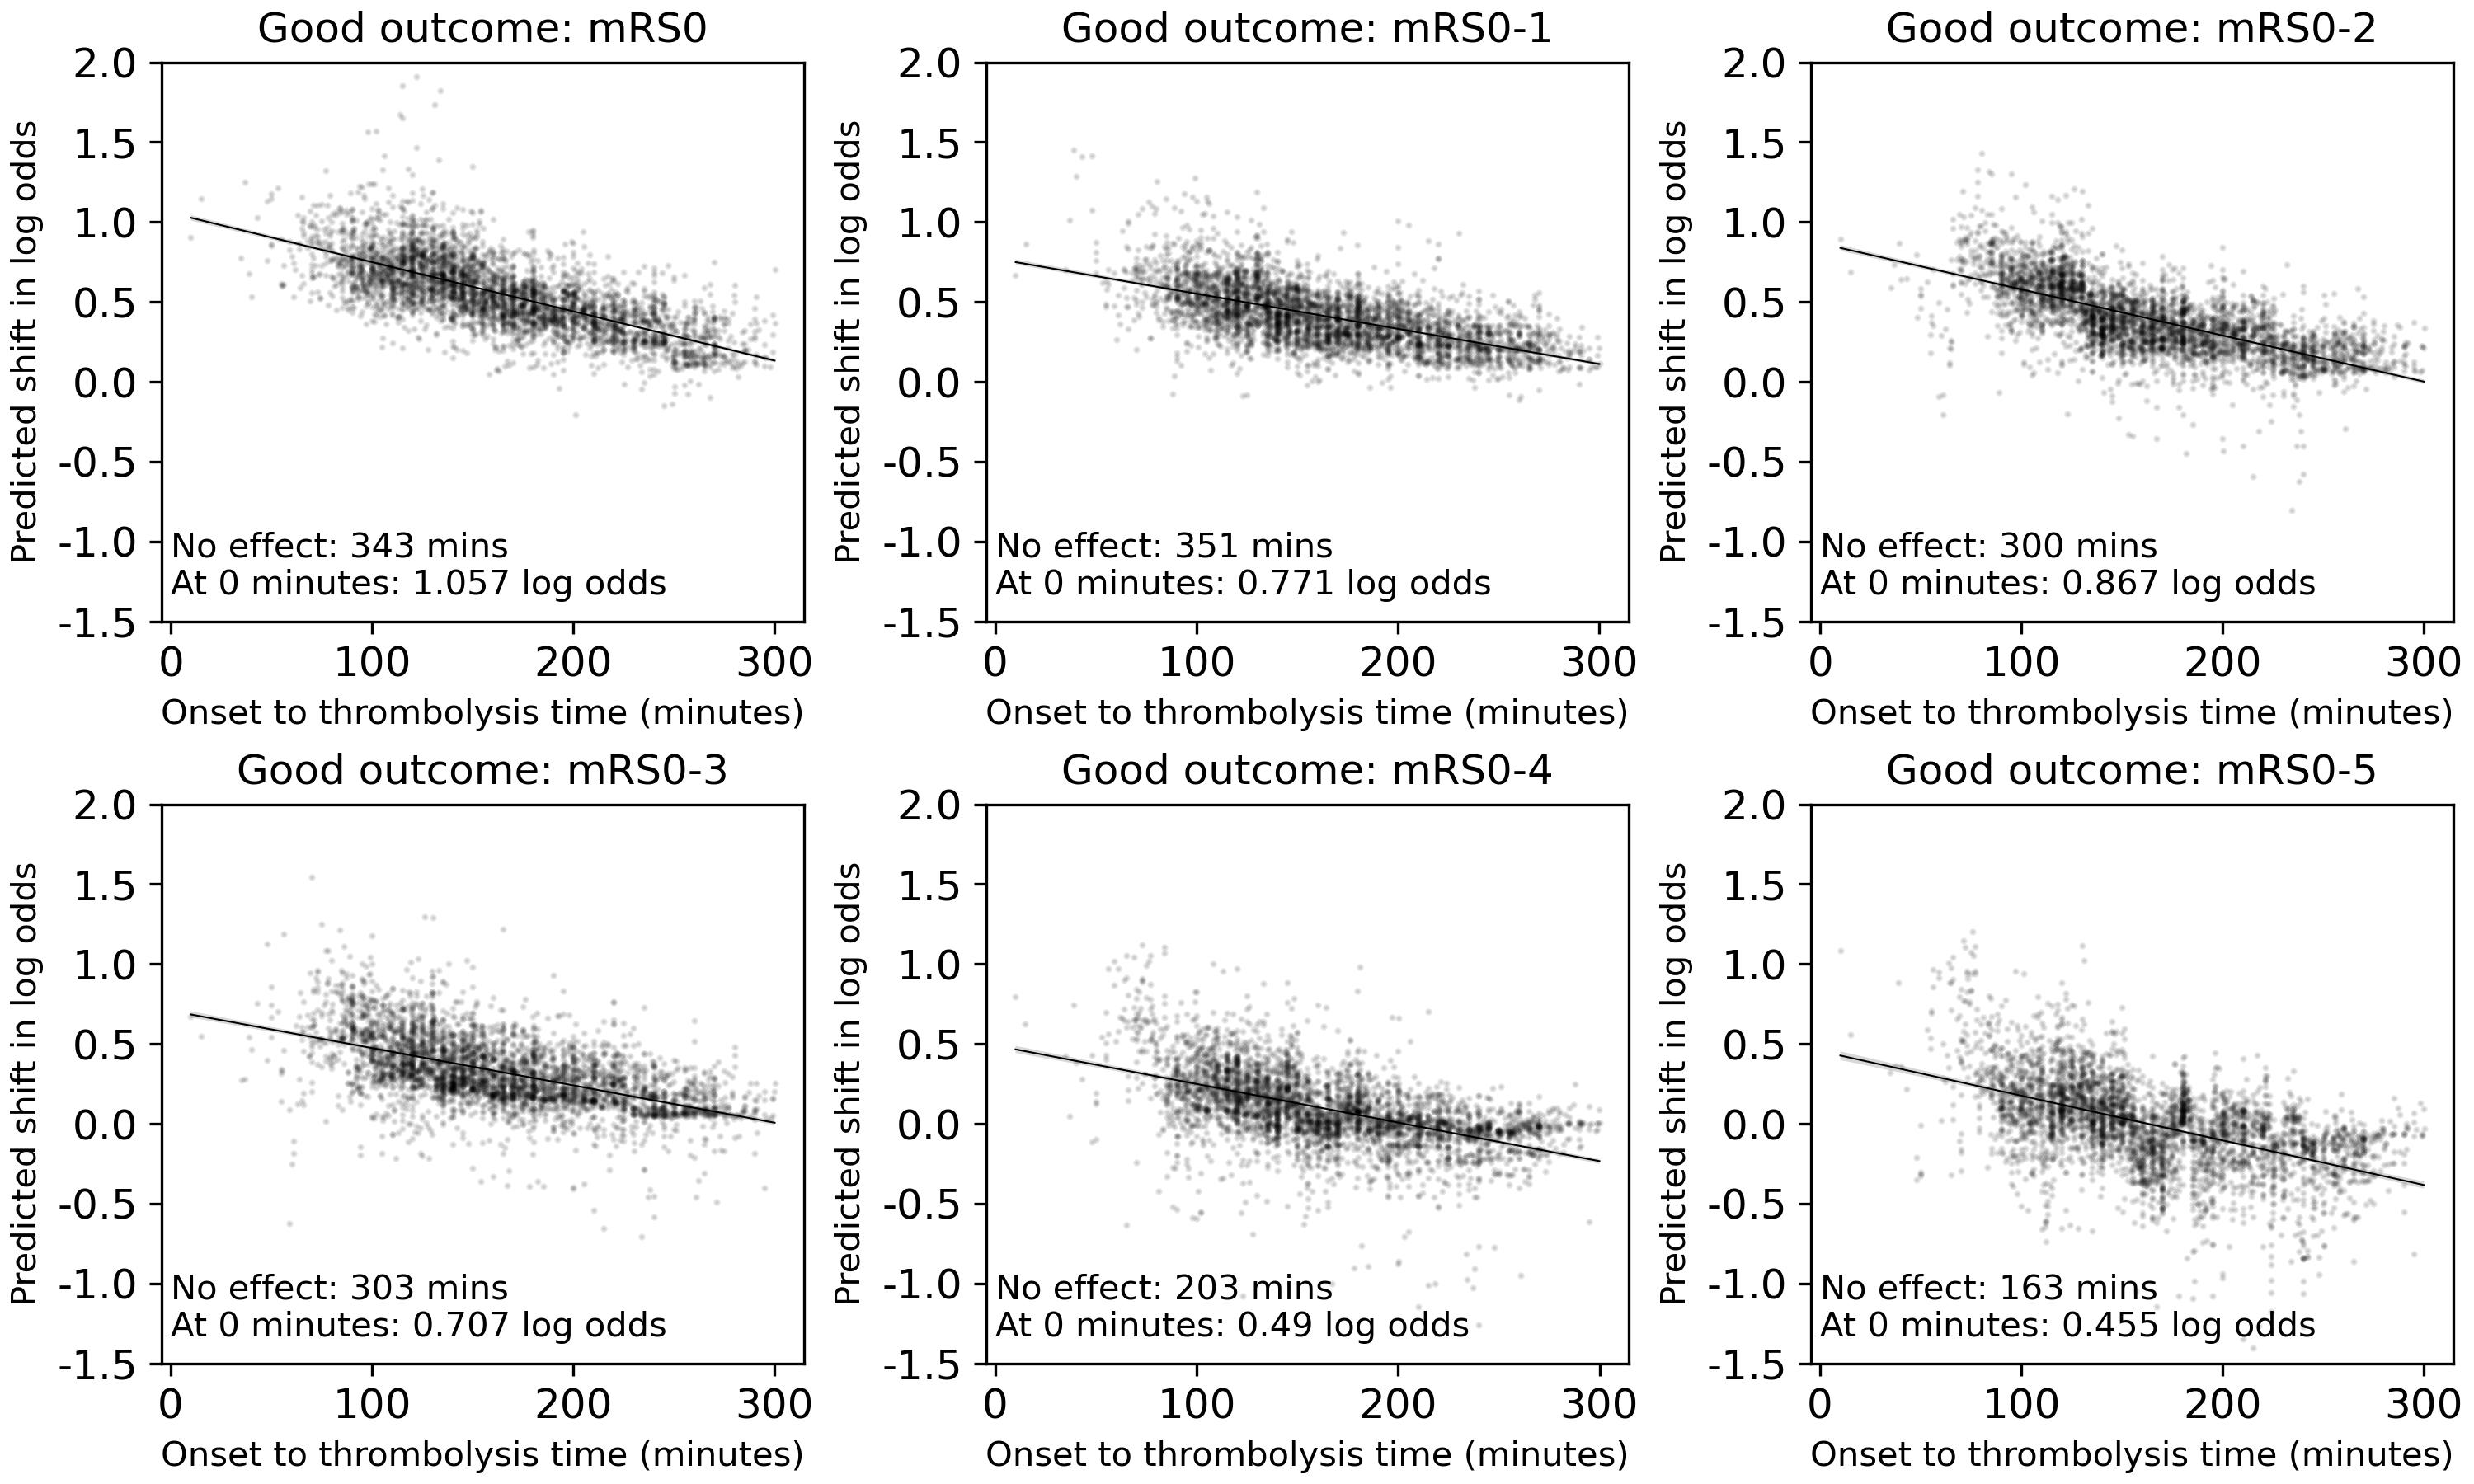
\includegraphics[width=1\textwidth]{./images/103_xgb_7_features_1fold_binary_improvement_logodds_bymRSthreshold_sns_6_subplots_nLVO_ivt_shap_paper}\\
      \caption{Patients in the test set that received thrombolysis with mild-moderate stroke (NIHSS 0-10)}
      \label{fig:shap_shift_nlvo}
    \end{subfigure}
    \label{fig:shap_shift}
    \caption{Fitting linear regression to the shift in the contribution from receiving thrombolysis towards having a good outcome at discharge with respect to the onset to thrombolysis time. A subplot for each mRS threshold used to define a good outcome.}
\end{figure}

\begin{table}[!ht]
    \caption{Fitting linear regression to the shift in the contribution from receiving thrombolysis towards having a good outcome (mRS 0-1) at discharge with respect to the onset to thrombolysis time. Linear regression statistics for different patient cohorts, and different definitions of a good outcome. We used NIHSS 0-10 to define mild-moderate strokes, and NIHSS 11+ to define severe strokes. }
%    \begin{subtable}[b]{1\textwidth}
%          \caption{Good outcome defined using all six mRS thresholds (common odds ratio).}
%    \centering
%        \begin{tabular}{lllllllll}
%        \toprule
%         & Variables & coef & std err & t & P$>$$|$t$|$ & [0.025 & 0.975] \\ 
%         \midrule
%        All ischaemic stroke & Constant  & 0.8596 & 0.004 & 202.579 & 0.000 & 0.851 & 0.868\\
%        & Onset to IVT time (mins) & -0.0031 & 2.52e-05 & -122.600 & 0.000 & -0.003 & -0.003\\ 
%        \midrule
%        Severe stroke & Constant  & 0.9971  &    0.006 &   174.202  &    0.000    &   0.986   &    1.008\\
%        & Onset to IVT time (mins) & -0.0027  &  3.3e-05 &   -83.259  &    0.000   &   -0.003    &  -0.003\\ \midrule
 %       Mild-moderate stroke & Constant & 0.7245 & 0.006 & 126.085 & 0.000 & 0.713 & 0.736\\
 %       & Onset to IVT time (mins)  &  -0.0026 &  3.33e-05 &   -78.747  &    0.000 &     -0.003  &    -0.003\\
 %       \bottomrule
 %       \end{tabular}

 %     \label{fig:stats_table_common_odds_ratio}
 %   \end{subtable}
 %   \par\bigskip % force a bit of vertical whitespace
%    \begin{subtable}[b]{1\textwidth}
%    \caption{Good outcome defined as mRS 0-1.}
    \centering
        \begin{tabular}{lllllllll}
        \toprule
         & Variables & coef & std err & t & P$>$$|$t$|$ & [0.025 & 0.975] \\ 
         \midrule
        All ischaemic stroke & Constant & 0.9012 & 0.007 & 132.519 & 0.000 & 0.888 & 0.915\\
        & Onset to IVT time (min) &  -0.0027  & 4.04e-05 & -68.058 & 0.000 & -0.003 & -0.003\\   
        \midrule
        Severe stroke & Constant & 1.0476  &    0.011  & 96.746 & 0.000 & 1.026 & 1.069\\
        & Onset to IVT time (mins) & -0.0033 &  6.67e-05  & -50.042 & 0.000 & -0.003 & -0.003\\ 
        \midrule
        Mild-moderate stroke & Constant &           0.7708 &     0.008   & 97.613 & 0.000 & 0.755 & 0.786\\
        & Onset to IVT time (mins) &  -0.0022 &   4.57e-05 & -48.109 & 0.000 & -0.002 & -0.002\\
        \bottomrule
        \end{tabular}

      \label{fig:stats_table_mrs1}
%    \end{subtable}
   
\end{table}


Here is the secondary analysis that repeats the analysis in the paper that uses the full log-odds change in achieving a given mRS threshold with and without thrombolysis (instead of the log-odds change associated with the thrombolysis use feature). Using the full model prediction, rather than isolating the effect of thrombolysis using thrombolysis SHAP, produced similar results, but with a little larger predicted effect of thrombolysis (e.g  maximum theoretical beneficial of thrombolysis of improving the log odds of being discharged mRS 0-2 of 1.1 (\textit{c.f.} 0.90 when using the isolated effect of thrombolysis from the thrombolysis SHAP values, with no-effect time being 328 minutes and 334 minutes for the isolated and full effect models).

\begin{figure}[!ht]
    \centering
    \begin{subfigure}[b]{1\textwidth}
      \centering
      \includegraphics[width=1\textwidth]{./images/103_xgb_7_features_1fold_binary_improvement_logodds_bymRSthreshold_sns_6_subplots_nLVO_LVO_total_shap_paper}\\
      \caption{Patients in the test set that received thrombolysis}
      \label{fig:shap_shift_lvo_nlvo_full_model_prediction}
    \end{subfigure}
    \hfill
    \begin{subfigure}[b]{1\textwidth}
      \centering    
      \includegraphics[width=1\textwidth]{./images/103_xgb_7_features_1fold_binary_improvement_logodds_bymRSthreshold_sns_6_subplots_LVO_total_shap_paper}\\
      \caption{Patients in the test set that received thrombolysis with severe stroke (NIHSS 11+)}
      \label{fig:shap_shift_lvo_full_model_prediction}
    \end{subfigure}
    \hfill
    \begin{subfigure}[b]{1\textwidth}
      \centering
      \includegraphics[width=1\textwidth]{./images/103_xgb_7_features_1fold_binary_improvement_logodds_bymRSthreshold_sns_6_subplots_nLVO_total_shap_paper}\\
      \caption{Patients in the test set that received thrombolysis with mild-moderate stroke (NIHSS 0-10)}
      \label{fig:shap_shift_nlvo_full_model_prediction}
    \end{subfigure}
    \label{fig:shap_shift_full_model_prediction}
    \caption{Fitting linear regression to the shift in the full model prediction from receiving thrombolysis towards having a good outcome at discharge with respect to the onset to thrombolysis time. A subplot for each mRS threshold used to define a good outcome.}
\end{figure}


\begin{table}[!ht]
%    \begin{subfigure}[b]{1\textwidth}
%    \centering
%        \begin{tabular}{lllllllll}
%        \toprule
%         & Variables & coef & std err & t & P$>$$|$t$|$ & [0.025 & 0.975] \\ 
%         \midrule
%        All ischaemic stroke & Constant  & 1.0387 & 0.008 & 138.005 & 0.000 & 1.024 & 1.053\\
%        & Onset to IVT time (mins) & -0.0036 & 4.47e-05 & -79.727 & 0.000 & -0.004 & -0.003\\ 
%        \midrule
%        Severe stroke & Constant  & 1.2973  &    0.011 &   119.862  &    0.000    &   1.276 & 1.319\\
%        & Onset to IVT time (mins) & -0.0042  &  6.67e-05 &   -63.065  &    0.000   &   -0.004    &  -0.004\\ \midrule
%        Mild-moderate stroke & Constant & 0.7803 & 0.010 & 80.932 & 0.000 & 0.761 & 0.799\\
%        & Onset to IVT time (mins)  &  -0.0027 &  5.58e-05 &   -48.286  &    0.000 &     -0.003  &    -0.003\\
%        \bottomrule
%        \end{tabular}
%      \caption{Good outcome defined using all six mRS thresholds (common odds ratio).}
%      \label{fig:stats_table_common_odds_ratio_full_model_prediction}
%    \end{subfigure}
%    \par\bigskip % force a bit of vertical whitespace
%    \begin{subfigure}[b]{1\textwidth}
    \centering
        \begin{tabular}{lllllllll}
        \toprule
         & Variables & coef & std err & t & P$>$$|$t$|$ & [0.025 & 0.975] \\ 
         \midrule
        All ischaemic stroke & Constant & 1.0992 & 0.016 & 68.965 & 0.000 & 1.068 & 1.130\\
        & Onset to IVT time (min) &  -0.0033  & 9.46e-05 & -34.778 & 0.000 & -0.003 & -0.003\\   
        \midrule
        Severe stroke & Constant & 1.3797  & 0.027  & 51.601 & 0.000 & 1.327 & 1.432\\
        & Onset to IVT time (mins) & -0.0044 &  0.000  & -26.845 & 0.000 & -0.005 & -0.004\\ 
        \midrule
        Mild-moderate stroke & Constant &           0.8494 & 0.018   & 46.756 & 0.000 & 0.814 & 0.885\\
        & Onset to IVT time (mins) &  -0.0022 &   0.000 & -21.301 & 0.000 & -0.002 & -0.002\\
        \bottomrule
        \end{tabular}
      \label{fig:stats_table_mrs1_full_model_prediction}
%    \end{subfigure}
    \caption{Fitting linear regression to the shift in the full model prediction from receiving thrombolysis towards having a good outcome (mRS 0-1) at discharge with respect to the onset to thrombolysis time. Linear regression statistics for different patient cohorts, and different definitions of a good outcome. We used NIHSS 11+ to define a severe stroke, and NIHSS 0-10 to define mild-moderate stroke.}
\end{table}




%\FloatBarrier
